\documentclass{article}
\usepackage{iclr2027_conference,times}
\usepackage{amsmath,amssymb,amsthm,booktabs,graphicx,multirow}
\usepackage{placeins,float}
\usepackage{hyperref,url}
\hypersetup{hidelinks}
\newcommand{\E}{\mathbb{E}}
\newcommand{\Prb}{\mathbb{P}}
\newcommand{\ind}{\mathbf{1}}
\newtheorem{proposition}{Proposition}
\newtheorem{theorem}{Theorem}
\newcommand{\wape}{\operatorname{WAPE}}
\newcommand{\StrongRiskSentence}{86.30\% mean acceptance for contract excess versus 80.22\% for forecast-normalized error, with accepted WAPE 0.6245 and 0.6216, respectively. The first-seed coverage gain is 6.04 percentage points (descriptive paired interval [5.39, 6.68]).}
\newcommand{\StrongGroupSentence}{The stronger forecast improves the pooled acceptance result but retains category failures: Hobbies accepted WAPE is 0.8442 and Household is 0.6788, both above the unchanged cap. Category-specific screening still returns no Hobbies candidate.}

\newcommand{\ObservableMainSentence}{The sales-and-capacity negative-binomial control selects shape $\kappa=2$ in all three fits. Its excess rule accepts 48.17\% of shadow rows and covers 54.80\% of demand, with WAPE 0.5461. Pooled point estimates pass in all three periods, but Hobbies shadow WAPE is 0.8018, above the 0.64013 cap. }

\title{When More Predictions Cover Less:\\Accuracy and Coverage under Ratio Risk}
\author{Anonymous authors}
\begin{document}
\maketitle
\begin{abstract}
Under a ratio-risk constraint, accepting more predictions can cover less exposure. We develop a budget audit of this mismatch: accurate high-exposure cases supply error slack for inaccurate low-exposure cases. Sharp examples, bounded-exposure limits, and non-reversal conditions delimit the mechanism; a conditional perturbation bound relates head accuracy to decision accuracy under explicit assumptions. Across three training seeds and four complete-sales retail head settings, exposure selection gains 7.78--12.05 coverage points while losing 15.81--36.54 case points. The exchange persists without artificial censoring. External tests on Dominick's oatmeal, Bibtex, and Mediamill, with protocols frozen before raw-data download, show the same point direction but all fail their declared joint coverage-and-screening criterion. Bibtex's net case loss is confined to forced single-label rows; Mediamill retains a point exchange without those rows but fails risk screening. A direct learned gate improves observed Bibtex coverage but also fails screening. These findings separate prediction accuracy, acceptance utility, and risk assessment without establishing population risk guarantees.
\end{abstract}

\section{Introduction}
Selective prediction must specify both risk and acceptance utility. Case coverage gives each case equal value; exposure coverage weights its opportunity or demand mass. Under a ratio of accepted loss to accepted weight, that choice becomes part of the learning problem.

Case coverage can increase while covered exposure falls. Equal value per case remains a legitimate objective, but cannot stand in for exposure coverage. The threshold rankings are established; our contribution is to quantify their disagreement. We give nearly maximal joint gaps, a bound under bounded exposure, and conditions excluding reversal. The acceptance unit matters: fixed multi-label prediction with whole-example abstention can reverse the objectives, whereas ordinary binary precision with an unrestricted gate admits a common optimum.

Retail WAPE makes the mechanism concrete. Well-predicted high-volume cases create pooled error slack that pays for many poor low-volume predictions. Our main experiment refits matched retail pipelines with artificially censored and complete recorded sales. It measures the coverage mismatch without proposing a new forecasting architecture. Frozen external tests extend the audit to another retailer and to multi-label micro-precision; archived mobility and forecasting comparisons have supplementary roles.

We compare case and exposure utility on a shared five-rule menu. Paired refits test the role of artificial censoring; calibration audits vary fitted heads, secondary utility, and the case floor. Accepted-set accounting explains the resulting budget allocations. The M5 analyses are retrospective. Three external tests separate coverage exchange from risk-screen passage, and direct learned gates test acceptance estimation with the classifier held fixed. All external joint criteria are reported, including nonattainment.

\section{Related work and scope}
\paragraph{Count-data evaluation.}
\citet{kolassa2016count} explains why absolute-error measures, including weighted MAPE, can be unsuitable for retail count forecasts. Absolute loss elicits a median; when $\Pr(Y=0)\geq1/2$, zero is a median. Our new object is the acceptance budget: a poor relative-error row may still be inexpensive to accept. M5 established strong tabular forecasting baselines \citep{makridakis2022m5}; we use LightGBM \citep{ke2017lightgbm}. Mechanical censoring preserves complete evaluation targets; it is not a theoretical premise. Appendix~\ref{app:natural-diagnostics} covers natural-stockout identification.

\paragraph{Ratio metrics and selective prediction.}
Optimization of nondecomposable and ratio-of-linear classification metrics is well established \citep{dinkelbach1967,koyejo2014,narasimhan2015complex,bao2020fractional}. We instead fix the predictor and quantify disagreement between acceptance utilities under one ratio constraint.

\paragraph{Selection and risk control.}
Case coverage and its risk trade-off are foundational to selective classification \citep{elyaniv2010foundations,geifman2017selective}. SelectiveNet jointly trains prediction and rejection end to end \citep{geifman2019selectivenet}; our custom fixed-predictor gates compare acceptance estimation without reproducing joint SelectiveNet training. Conditional-loss thresholding is established in reject-option prediction \citep{franc2023reject}, as are group concerns in selective regression \citep{shah2022selective}. \citet{jones2021} show that selective classification can magnify group disparities. \citet{fisch2022} study calibration within the selected population; our distinct question is which population mass coverage rewards. Learn then Test and conformal risk control address calibration under explicit assumptions \citep{angelopoulos2021ltt,angelopoulos2024crc}. \citet{joshi2026postprocess} preserve agreement with a baseline policy under a chance constraint. We instead compare acceptance utilities under pooled signed excess $\E[a(e-r\mu)]\leq0$: accurate high-volume cases can subsidize inaccurate low-volume cases. Conditional thresholding is the shared mathematical tool; the distinct object here is the measurable disagreement between coverage utilities.


\section{The acceptance constraint}
% Replaces main.tex Section 3.1. Reserve Proposition 1 for Appendix A.
\subsection{Utility mismatch under ratio risk}
Let $X$ be the information available when acceptance is chosen. For
nonnegative integrable loss $L$ and exposure $W$, define
\[
 \ell(X)=\E[L\mid X],\quad w(X)=\E[W\mid X],\quad T=\E W>0,
 \quad a(X)\in[0,1].
\]
Row coverage, exposure coverage, and accepted ratio risk are
\begin{equation}
 c(a)=\E a,\qquad d_W(a)=\frac{\E[aW]}{T},\qquad
 R(a)=\frac{\E[aL]}{\E[aW]}.
 \label{eq:ratio}
\end{equation}
The accepted denominator must be positive. The acceptance constraint is $R(a)\leq r$
and $c(a)\geq c_0$. Its signed excess is
\begin{equation}
 g_r=L-rW,\qquad m_r=\ell-rw,\qquad
 R(a)\leq r\ \Longleftrightarrow\ \E[a m_r]\leq0.
 \label{eq:excess}
\end{equation}
WAPE is the specialization $L=|Y-f(X)|$, $W=Y$, with $Y,f\geq0$;
then $\ell=e$, $w=\mu$, and $d_W=d$ is demand coverage.

Fixed-row-coverage excess is minimized by accepting the smallest
$m_r$ values, with randomization on ties (Proposition~\ref{prop:threshold}
in Appendix~\ref{app:proofs}). To maximize exposure instead, change measure
to $d\nu=w\,dP_X/T$ after rejecting $w=0,\ell>0$ contexts: then $d_W(a)=\E_\nu a$ and
$R(a)=\E_\nu[a\ell/w]/\E_\nu a$.
\setcounter{proposition}{1}
\begin{proposition}[Exposure-weighted ranking]
\label{prop:weighted}
If a positive-exposure feasible rule exists and the row floor is
nonbinding, exposure coverage is optimized by thresholding $\ell/w$,
with boundary randomization. Reject $w=0,\ell>0$ contexts; $w=\ell=0$
contexts are neutral for this objective. The ranking is independent of
$r$; its threshold is not.
\end{proposition}
Thus the population rankings are $\ell-rw$ for rows and $\ell/w$ for
exposure. A fixed ranking's largest feasible threshold maximizes either
coverage because its acceptance sets are nested; objective comparisons
must therefore also compare ranking families (Appendix~\ref{app:objective}).

For disjoint context sets $K,U$, write
\[
 M_A=\E[\ind_Aw],\qquad B=-\E[\ind_Km_r],\qquad
 M_K>0,\quad B\geq0.
\]
Here $B$ is the excess slack supplied by a common accepted set.
\begin{proposition}[Sharp objective reversal for ratio risk]
\label{prop:lowdemand}
Fix $r>0$, $\rho>r$, and $\varepsilon>0$. If $\ell=\rho w$ on $U$ and
$0<M_U\leq\varepsilon\Pr(U)$, then $R(\ind_U)=\rho$ and
$K\cup U$ satisfies the cap exactly when $(\rho-r)M_U\leq B$.
Accepting $U$ adds $\Pr(U)$ row coverage but at most
$\varepsilon\Pr(U)/T$ exposure coverage.

For every $0\leq c_0<1$ and $\eta>0$, there exists a three-context
law with $w>0$, $0\leq\ell\leq\rho w$, and exact conditional moments
whose unique row- and exposure-optimal policies $a_R,a_W$ satisfy
the cap and the nonbinding row floor, and obey
\[
 c(a_R)-c(a_W)>1-c_0-\eta,\qquad
 d_W(a_W)-d_W(a_R)>1-\eta.
\]
The universal bounds $1-c_0$ and $1$ are jointly sharp. For
$0<r<1$ and $\rho=1$, this sharpness also holds with binary $0\leq L\leq W\leq1$.
\end{proposition}
Approaching the joint bounds uses a sequence with vanishing conditional exposure; the construction does not establish typical or nondegenerate empirical gaps. The sharpness statement ranges over joint laws that can realize the
conditional moments in Appendix~\ref{app:proofs}; it is not a claim
about every fixed metric class. If $W$ is constant, for example,
$d_W=c$ and reversal is impossible. For a fixed multi-label classifier, whole-example abstention yields an exact micro-precision reversal (Appendix~\ref{app:classification}). Ordinary binary precision with an unrestricted gate instead has a common optimum for both coverage objectives. For whole-example micro-precision with $1\leq w\leq m$, each coverage gap is at most $(m-1)/(m+1)$; Appendix~\ref{app:bounded_exposure} sharpens this to a joint bound.

\paragraph{When reversal is limited or absent.}
For row- and exposure-optimal policies on a common feasible set, let
$x=c(a_R)-c(a_W)\geq0$ and $y=d_W(a_W)-d_W(a_R)\geq0$.
If $0<u\leq w\leq v$, then, with $D=(v-u)/(v+u)$,
\begin{equation}
 y\leq\frac{D-x}{1-Dx},\qquad 0\leq x,y\leq D.
 \label{eq:bounded}
\end{equation}
Thus constant positive conditional exposure rules out reversal. Moreover,
with unrestricted randomized acceptance under just the pooled risk cap and row
floor, at most two positive-probability, positive-exposure contexts have a common
optimum whenever feasible. Strict reversal requires at least three such contexts.
Appendix~\ref{app:bounded_exposure} proves both claims; variation alone is not
sufficient, as $\ell\equiv0$ makes accept-all optimal for any exposure.

\paragraph{WAPE corollary and estimation.}
For $0<r<1$, setting $\rho=1$, $W=Y$, and $f=0$ on $U$ gives
$e=\mu$: near-zero-demand rows have budget cost $(1-r)\mu$ yet
unit row reward. The three-context law is realizable by deterministic
nonnegative forecasts (Appendix~\ref{app:proofs}), so both sharp bounds
hold for WAPE. A low-exposure share alone cannot bound the forgone
exposure without a positive excess-rate margin; the appendix gives
that bound and the exact budget identity. More generally $|e-\mu|\leq f$.
Exact-head optimality does not imply estimated-ratio robustness.
Section~\ref{sec:objectives} and Appendix~\ref{app:proofs} distinguish
objective alignment from small-denominator error amplification.

\paragraph{From head error to decision error.}
Small head error alone does not ensure small coverage regret: Appendix~\ref{app:plugin-v12} gives a two-context example with vanishing error and a limiting $1/2$ coverage loss. A conditional perturbation bound controls coverage and risk when a strictly feasible comparator and positive accepted exposure exist. This specializes established constraint-sensitivity arguments; its assumptions do not certify the fitted menu.

\subsection{A fixed classifier: examples versus positive predictions}
\label{sec:classification}
Consider a fixed two-label classifier with whole-example abstention. Exposure $W$ counts its positive predictions, and loss $L$ counts false positives, so $1-R$ is accepted micro-precision. Three contexts have the following known conditional moments:
\[
\begin{array}{c|ccc}
 &K&U&V\\\hline
 \Pr(X)&2/5&2/5&1/5\\
 h(X)&(1,0)&(1,0)&(1,1)\\
 w(X)&1&1&2\\
 \ell(X)&0&3/10&1/2
\end{array}
\]
At risk cap $r=1/10$ and case floor $c_0=7/20$, every optimum accepts $K$. Its risk surplus funds the remaining constraint $4a_U+3a_V\leq2$. Maximizing accepted examples chooses $(a_K,a_U,a_V)=(1,1/2,0)$, giving $(c,d_W)=(3/5,1/2)$. Maximizing accepted positive predictions instead chooses $(1,0,2/3)$, giving $(8/15,5/9)$. Both attain exactly 90\% micro-precision. The classifier is unchanged; only the value assigned to acceptance differs (Figure~\ref{fig:mechanism}). Appendix~\ref{app:classification} specifies the label distribution and verifies both optima.

For ordinary binary precision, accepting all predicted-negative cases costs no risk budget, and completed gates satisfy $c=1-T+Td_W$. Both objectives then have a common optimum. This contrast makes the acceptance unit consequential: gating each label separately would change the multi-label problem above.

\begin{figure}[t]
\centering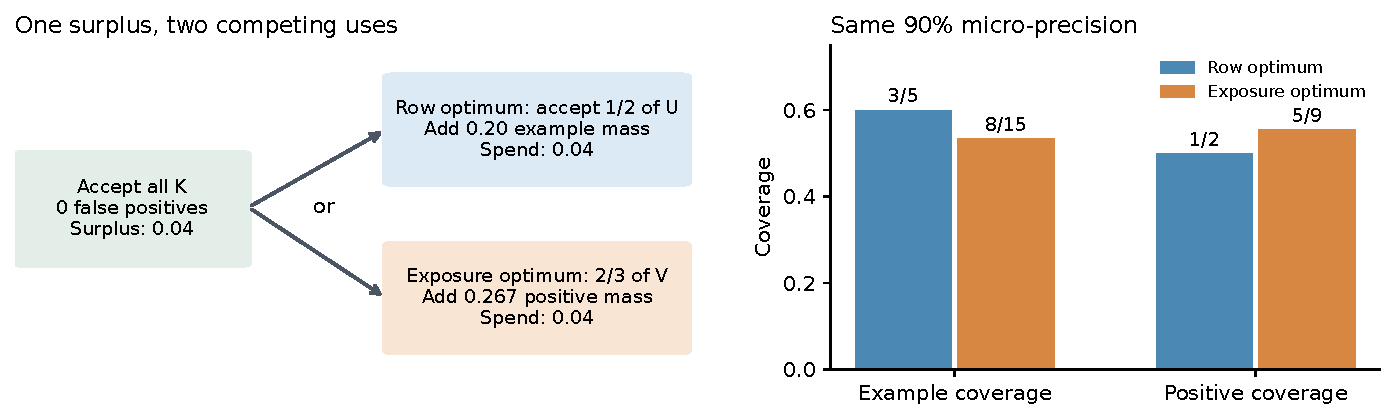
\includegraphics[width=\linewidth]{figures/utility_mechanism.pdf}
\caption{Exact fixed-classifier example, not an empirical benchmark. Left: the accurate context $K$ supplies 0.04 expected excess units; either competing allocation uses all of them. Right: the same risk budget buys more examples or more positive predictions, but not both. Fractional acceptance is independent randomization within a context.}
\label{fig:mechanism}
\end{figure}



\paragraph{Scope under censoring.}
The mismatch theorem does not require censored observations. Its inputs are the conditional loss and exposure of a fixed predictor. Mechanical censoring lets us retain the complete target to estimate and audit these inputs; natural stockouts generally do not. Observed sales alone cannot certify a cap below one when compatible demand tails are unbounded (Appendix~\ref{app:identification}). This is a limit on identifying the theorem's inputs, not an additional explanation of objective reversal.

\subsection{Calibration is a separate claim}
\label{sec:calibration}
Independent calibration clusters and known bounded cluster losses permit simultaneous finite-family concentration checks; the supplement states a standard Hoeffding construction (Appendix~\ref{app:calibration}). Our retail counts lack a justified population bound and share store/calendar shocks. Accordingly, development intervals are descriptive; the M5 comparisons use prespecified item-bootstrap approximations, not that theorem; external resampling schemes are stated separately.

\section{Primary paired audit}
\subsection{Data, predictors, and chronology}
The main experiment uses 1,829 M5 items across ten stores (18,290 series). Two median-loss LightGBM pipelines share feature definitions, sampled rows, and model budgets. One uses artificially censored sales for histories and predictor targets; the other uses complete recorded sales. Both exclude capacity, fill, and hit features. Each 300-tree predictor fits 600,000 rows on days 1314--1554. Squared-loss error and exposure heads fit 600,000 rows on days 1555--1610. Their 220/660-tree factorial supplies four settings per arm. The protocol specifies the primary relative cap and full factorial; 220/220 is a reference, not a separately prespecified primary cell. Tree counts are not selected by validation or early stopping.

Calibration A/B spans days 1611--1645 and 1646--1673; evaluation spans days 1800--1913 (2,085,060 rows), called Later in saved tables. The original paired fits use seed 20260910; two additional seeds, 20260913 and 20260914, repeat all ten fits each under a recorded specification. They change sampled training rows as well as learner randomness. Table~\ref{tab:matched-history} reports all three seeds; subsequent calibration and budget diagnostics retain the original seed. Appendix~\ref{app:matched} specifies the fits; Table~\ref{tab:experiment-map} maps the two paired predictors, archived L1/residual/Chronos comparisons, and new calibration audits to their separate protocols.

Recorded M5 sales are the target $Y$. After 56 uncensored warmup days, the fixed mechanical process gives
\begin{align}
 L_t&=0.90L_{t-1}+0.10S_{t-1},&
 C_t&=\max\{1,\lceil1.15L_t+0.25\sqrt{L_t+1}\rceil\},&
 S_t&=\min(Y_t,C_t).
 \label{eq:censor}
\end{align}
It hides 30.42\% of recorded sales mass and censors 12.67\% of development rows on days 1314--1913. Forecasts use origin-available information at horizons one through seven days. Retained complete targets train and calibrate both arms' audit heads. Removing artificial censoring does not remove possible natural stockouts from the original sales records or identify latent customer demand.

\subsection{A common menu, two selection utilities}
\label{sec:choice-design}
For each seed and arm, the primary cap is .95 times its maximum full-coverage risk over calibration windows A and B; the original caps are .6647 for censored histories and .6327 for complete sales. Relative factors $\{.85,.90,.95,1,1.05\}$ match strictness relative to each arm. A separate absolute grid compares common risk levels, including .64012983268, the reporting cap of the archived study. Neither cap construction is a retail standard. Appendix~\ref{app:matched} reports every setting, including infeasible and accept-all outcomes.

The shared five-rule menu ranks conditional absolute error $\hat e$, row excess $\hat e-r\hat\mu$, exposure-normalized error, descending predicted exposure $-\hat\mu$, or mixed utility. The conditional-error comparator uses regression-based uncertainty estimation \citep{franc2023reject}, recalibrated to our ratio cap; it does not reproduce SELE training. For $U_\lambda=\lambda c+(1-\lambda)d$ and a nonbinding row floor, mixed utility orders
\begin{equation}
 s_\lambda=\frac{\hat e-r\hat\mu}{\lambda+(1-\lambda)\hat\mu/T},\qquad
 \lambda\in\{1,.25,0\},
 \label{eq:mixed}
\end{equation}
where $T$ is a fixed head-training estimate of mean exposure. Positive-exposure ordering at zero is equivalent to $\hat e/\hat\mu$. The menu uses no denominator floor. For each ranking, all distinct calibration scores and accept-all are searched; the largest complete-tie threshold with empirical risk at most $r$ and case coverage at least .35 in both windows is retained. Infeasible candidates remain in the record. At the original primary caps, Error is infeasible in both paired arms and Bike; failed candidates remain reported.

Within one nested ranking, both coverages increase with the accepted prefix. Utility therefore selects between candidate rankings, not different thresholds along the same family. Among eligible candidates $j$, we choose
\begin{equation}
 j_C=\arg\max_j\min_{b\in\mathcal B}\widehat c_b(a_j),
 \qquad j_D=\arg\max_j\min_{b\in\mathcal B}\widehat d_b(a_j),
 \label{eq:menu-choice}
\end{equation}
with $\mathcal B=\{A,B\}$ and a fixed tie order. Evaluation labels enter neither choice. An empty eligible menu returns no policy and undefined accepted risk. This audits a finite menu, not all possible gates. All headline exchanges use Equation~\eqref{eq:menu-choice}; Equation~\eqref{eq:tolerance} is a retrospective alternative.

\subsection{Uncertainty and evidential scope}
The primary intervals use 2,000 paired item-bootstrap draws and descriptive 95\% percentiles. Resampling retains all stores and dates of each item but does not remove shared store/calendar shocks. These intervals condition on fitted predictors, heads, and selected policies; they omit training and selection uncertainty. Their nominal level is not a simultaneous-risk guarantee (Section~\ref{sec:calibration}). The paired fits use previously evaluated development data, so chronology within the new computation does not create a fresh confirmation trial.

Retrospective calibration audits hold fitted heads and reporting caps fixed: resampling measures selection stability, a tolerance rule specifies a secondary utility, and an A-design/B-screen procedure varies the row floor. Conditions are recorded before each new computation; all data had already been evaluated. Appendices~\ref{app:v7} and \ref{app:v8} give the full records. These original calibration audits add no fits. The external protocols in Section~\ref{sec:external-v12} were frozen before their respective raw-data downloads and compute each cap from A alone. Their resampling units and interval families differ and are reported explicitly.

\section{Results}
\subsection{The mismatch survives removal of artificial censoring}
\label{sec:matched}
\begin{table}[t]\centering\small
\caption{Paired audit across the original seed 20260910 and two newly fixed seeds (20260913, 20260914). Entries are means $\pm$ sample SD across three seeds, in percentage points; SD is not a confidence interval. Caps are recomputed per seed and arm. Head settings share fitted components. Complete-sales 220/220 variability includes the R/R/D rule switch. Exposure choices are listed in seed order (R: Ratio; D: Descending); the case choice is Excess throughout. Appendix~\ref{app:seeds-v12} preserves every seed/cell and cap.}\label{tab:matched-history}
\begin{tabular}{llcrr}\toprule
Arm & Trees $e/w$ & Exposure choices & $\Delta c$ & $\Delta d$\\\midrule
Censored & 220/220 & D/D/D & $-38.76\pm1.17$ & $+8.40\pm1.40$ \\
Censored & 660/220 & D/D/D & $-39.79\pm1.34$ & $+9.25\pm1.69$ \\
Censored & 220/660 & D/D/D & $-36.54\pm1.22$ & $+9.37\pm1.13$ \\
Censored & 660/660 & D/D/D & $-38.98\pm1.15$ & $+9.00\pm1.20$ \\
Complete & 220/220 & R/R/D & $-22.95\pm10.29$ & $+9.67\pm1.23$ \\
Complete & 660/220 & D/D/D & $-34.80\pm0.95$ & $+11.08\pm1.20$ \\
Complete & 220/660 & D/R/D & $-30.86\pm6.79$ & $+9.28\pm1.31$ \\
Complete & 660/660 & D/D/D & $-35.36\pm1.04$ & $+9.88\pm1.51$ \\
\bottomrule\end{tabular}\end{table}

All 24 seed/head/arm settings exhibit the exchange. Across twelve complete-sales cells, exposure utility gains 7.78--12.05 demand points and loses 15.81--36.54 case points; censored ranges are +7.05--11.19 and -40.66 to -35.71. Table~\ref{tab:matched-history} summarizes three seeds; Appendix~\ref{app:seeds-v12} reports every cell. Direction persists, but magnitude and rule choice vary: complete 220/220 case loss has a 10.29-point sample SD. The additional seeds measure training-procedure sensitivity on the same M5 windows, not new-data generalization.

Observed exchange ratios range from .223 to .615 in complete sales and .176 to .293 under censoring. All twelve matched seed/head point comparisons favor complete sales, without a claim of seed-inclusive confidence. The original four adjusted, fixed-policy intervals remain in Appendix~\ref{app:v8-exchange}; they do not cover training or reselection uncertainty. Arm-specific caps, predictors and rules differ, so these ratios are not causal or economic effects.

In the original seed, complete-history refitting lowers full-coverage WAPE from .6853 to .6630. At the common absolute cap .64013, complete sales also gains 8.75 demand points for 13.21 case points forgone. Figure~\ref{fig:matched-history} shows cap dependence and family switches, which explain non-monotone differences. At relative caps of one or more, both choices accept all and the gap vanishes.

\begin{figure}[t]\centering
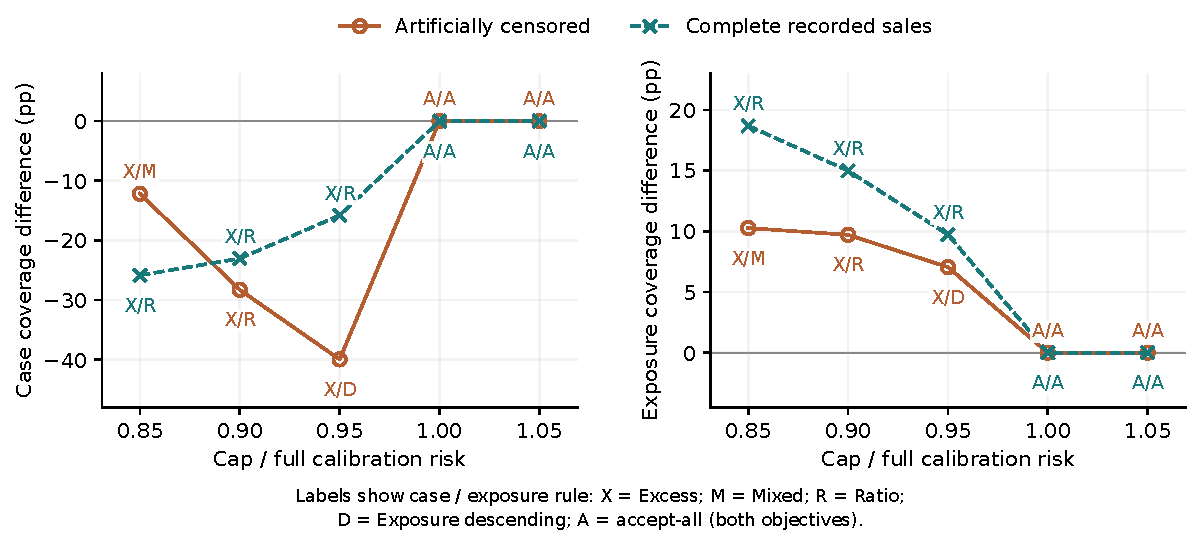
\includegraphics[width=\linewidth]{matched_history.pdf}
\caption{Original-seed (20260910) paired refits at 220/220. Tags identify the selected case/exposure rules at every point; coordinates show evaluation coverage differences. Rule changes explain non-monotone differences. The axis normalizes by each arm's maximum full A/B calibration risk. Overlapping accept-all points represent both arms. Table~\ref{tab:matched-history} summarizes three seeds; these original-seed lines connect declared caps, not Pareto frontiers.}\label{fig:matched-history}
\end{figure}

\subsection{Utility sensitivity and budget accounting}
\label{sec:head-intervention}\label{sec:selection-stability}\label{sec:tolerance}\label{sec:complete-screen}\label{sec:mass}
Original-seed diagnostics separate utility choice from estimation. At complete-sales 220/220, Ratio and Descending differ by only .027 calibration exposure points but 21.83 case points; 200 item-cluster redesigns select them in 51.5/48.5\% of draws. Untuned 660-tree heads change the choice without consistently improving MSE. A retrospective alternative values cases within an exposure allowance: for eligible candidates, let $\bar c_j=\min_b\widehat c_b(a_j)$ and $\bar d_j=\min_b\widehat d_b(a_j)$, and set
\begin{equation}
 \mathcal J_\varepsilon=\{j:\bar d_j\geq\max_k\bar d_k-\varepsilon\},
 \qquad j_{D,\varepsilon}=\mathop{\rm lexargmax}_{j\in\mathcal J_\varepsilon}(\bar c_j,\bar d_j).
 \label{eq:tolerance}
\end{equation}
Remaining ties retain the fixed order; case selection is unchanged. Every allowance in [.39,1.63] points selects Ratio in all four original-seed complete-sales cells. The illustrative .5-point choice gains 9.63--10.83 exposure points for 10.41--21.23 case points forgone; it is neither a recommended default nor an evaluation-loss bound. Under stricter A design at $.95r$ with $r=.632683$, Descending instead leads Ratio by 1.08--1.85 exposure points, outside this allowance. Raising the case floor from .35 to .40/.45 excludes Descending and selects Ratio. The separate B screen and Later risk summaries are approximate and conditional on fitted models. Figures, all floors, and exact allowance intervals remain in Appendices~\ref{app:v7}--\ref{app:v8}; headline results retain Equation~\eqref{eq:menu-choice}.

Accepted-set accounting describes how either utility spends the same budget. For a common set $K$ and disjoint added set $U$, with exposure mass $M$ and positive denominators,
\begin{equation}
 R_{K\cup U}\leq r \quad\Longleftrightarrow\quad M_U(R_U-r)\leq M_K(r-R_K).
 \label{eq:budget}
\end{equation}
The unscreened complete-sales 220/220 reference supplies 67,194 loss units of common-set slack. Its 485,906 case-only rows spend 74.72\%; 156,220 exposure-only rows carry over three times as much demand and spend 83.26\%. Their union exceeds the cap at its point estimate. Descriptive 95\% risk intervals for each policy and the union all cross the cap (Appendix~\ref{app:matched}). This accounting neither certifies population risk nor establishes Pareto-optimality; the conditional perturbation bound likewise requires unverified estimation, slack, and denominator assumptions (Appendix~\ref{app:plugin-v12}).

\subsection{Three frozen external tests and learned gates}
\label{sec:external-v12}\label{sec:external-v13}
The external studies use a common cap convention: $r=.95R_A(1)$, A design at $.95r$, and case floor .40. Each protocol was frozen before its raw-data download. A fixes the cap, candidate thresholds, and case/exposure choices; B only screens those fixed choices. This differs from the retrospective M5 primary A/B cap. The three studies retain different prediction tasks and resampling designs, so their gaps are not estimates of a dataset effect. All declared joint criteria require both selected policies to pass B and directional coverage intervals to exclude zero.

\begin{table}[t]\centering\small
\caption{The three frozen external-dataset tests, exposure choice minus case choice (percentage points). B status is shown for the case/exposure choices; every joint criterion is unmet. Dominick's uses paired 95\% four-week block intervals. Bibtex/Mediamill use 98.75\% row-bootstrap intervals adjusted over four contrasts; these levels and the separate screen families do not form one global 95\% claim. Mixed uses $\lambda=.5$ for Bibtex/Mediamill, versus .25 for Dominick's and M5; the non-WAPE .25 sensitivity is in Appendix~\ref{app:v13-nonwape}.}\label{tab:external-v13}
\begin{tabular}{llcll}\toprule
Dataset & Case / exposure & B & $\Delta c$ [interval] & $\Delta d$ [interval]\\\midrule
Dominick's & Excess / Ratio & pass/pass & $-4.63\ [-6.15,-3.45]$ & $+2.53\ [-.69,5.85]$\\
Bibtex & Excess / Ratio & pass/pass & $-4.41\ [-7.39,-1.55]$ & $+2.00\ [-1.84,6.08]$\\
Mediamill & Excess / Mixed & fail/fail & $-3.14\ [-4.27,-2.02]$ & $+2.40\ [1.31,3.57]$\\
\bottomrule\end{tabular}
\end{table}


Dominick's Oatmeal \citep{kiltsdominicks} has 4,839 store--UPC series from 66 products and 86 stores, with 85,039 Later records. Both selected policies pass B; the exposure interval includes zero (Appendix~\ref{app:external-v12}). Bibtex and Mediamill use fixed multi-label classifiers with whole-example abstention: exposure is the known predicted-positive count, loss is false-positive count, and risk is one minus micro-precision. A fixed .5 label threshold and top-one fallback ensure nonempty predictions. Bibtex passes B but does not confirm the exposure gain; Mediamill has both directional intervals excluding zero but fails B. Its eligible menu candidates have B point risks below the cap, so screen failure does not establish a risk violation. Descending is A-ineligible on both non-WAPE datasets: even its least-risk prefix satisfying the floor exceeds the reporting cap, unlike the M5 result. No prospective power calculation was documented for the two non-WAPE tests (Appendix~\ref{app:v13-nonwape}).

Retrospectively excluding fallback rows while retaining the fitted classifier and all policy choices changes Bibtex's exchange to $+.71/+7.00$ case/exposure points ($n=566$). Its net case loss is confined to forced single-label rows, which contribute $-41$ accepted cases versus $+4$ elsewhere. Mediamill retains a point exchange, $-1.78/+2.99$ ($n=4,169$). These subgroup summaries neither test a refitted no-fallback classifier nor inherit a new risk qualification. Appendix~\ref{app:v13-nonwape} retains the complete decomposition, alternative Mixed weight, and split-risk diagnostics.

Two custom primal--dual MLP gates per non-WAPE dataset use the same fixed classifier, feature information, and head-training rows as the menu. The Bibtex case gate improves Later case/exposure coverage by 6.56/6.99 points and lowers point risk from .40405 to .39922, but fails B; on B its point risk is .40247 versus .38342 for Excess. The other Bibtex gate also fails B. Mediamill's case gate is A-ineligible; its exposure gate gives $-1.81/+1.15$ points and fails B. No gate meets both eligibility and screening. These results establish neither menu nor gate superiority under the declared risk criterion and do not reproduce SelectiveNet's joint training.

\FloatBarrier
\section{Discussion}
\paragraph{Choose utility before choosing a score.}
The exact-information theorem does not prescribe the best estimated selector. Specify what acceptance rewards, compare a common menu under the same cap, and report both coverages. Equal value per case is a legitimate objective. An exposure gain cannot alone justify the associated case losses; the exchange ratio summarizes that trade, not a universal ordering of policies. In the original-seed complete-sales comparisons, Ratio's empirical value lies in covering more cases at similar or slightly lower exposure, with exposure allowances, higher case floors, and stricter-cap eligibility providing distinct, design-dependent routes to its selection.

\paragraph{What the theoretical bounds describe.}
The sharp construction bounds worst-case disagreement, not typical retail gaps. The bounded-exposure envelope needs a defensible positive lower bound. The finite two-label example reverses the objectives without vanishing exposure; binary precision and two-context laws delimit where reversal is impossible.

\paragraph{Fitted scores and secondary utility.}\label{sec:objectives}\label{sec:groups}
Exact-head rankings do not rank estimated policies. Equation~\eqref{eq:menu-choice} expresses pure case or exposure utility; Equation~\eqref{eq:tolerance} expresses case utility within an exposure allowance. Practice requires choosing this preference before outcomes are inspected; .5 points is not a recommended default. Its calibration allowance does not bound evaluation loss. At stricter relative caps .85/.90, Descending is infeasible. Complete-sales Ratio exceeds feasible runner-up Mixed by 4.01/3.43 calibration exposure points, but this is not a direct comparison with a feasible Descending or a causal test of error-head value (Appendix~\ref{app:v8-strict}). The non-WAPE prefix failures show that this estimated-rule ordering does not transfer unchanged across tasks.

\paragraph{Prediction, utility, and risk are separate tasks.}
Improving the predictor can enlarge what is feasible; choosing acceptance utility determines how that capacity is used. Neither step validates population risk. The primary sample-level budget findings and the separate approximate risk screen must retain their distinct scopes. Covered recorded sales are not measured profit, latent demand, or inventory-cost savings; an operational decision requires its own cost objective and validation.

\section{Limitations}
M5 uses three seeds on previously evaluated data; two were fixed after the original result. This coarsely describes training variability, not new-data generalization. The three external studies each use one learner seed and all miss their declared joint criteria. Local timestamped protocols are not public-registry preregistrations. Bootstrap summaries condition on fitted policies: M5 item resampling omits common calendar shocks; Dominick's weekly blocks retain co-movement but need stationarity assumptions; non-WAPE row resampling does not resolve feature overlap or unknown shot dependence. The two non-WAPE tests had no documented prospective power design. Fallback and menu conventions affect Bibtex's result; empirical exposure dispersion does not explain the cross-dataset gaps. The allowance is illustrative, heads are untuned, and Error is infeasible at the original M5 caps. Custom gates are one untuned architecture, not SELE or SelectiveNet. They neither establish a general selector ranking nor explain estimated Ratio's losses to Descending. No empirical screen is a population guarantee. Natural-stockout identification remains separate (Appendix~\ref{app:natural-diagnostics}); vanishing-exposure worst cases do not estimate observed gaps.

\section{Conclusion}
More accepted predictions need not cover more exposure. Three-seed paired refits preserve this mismatch without artificial censoring. Utility sensitivity and conditional bounds delimit the interpretation. Three frozen external studies show the same point direction but fail their joint criteria for distinct reported reasons; non-WAPE diagnostics and learned gates expose dependence on task and estimation choices. Specify utility, report both coverages and uncertainty, and assess risk separately.

\label{end:main}

\clearpage
\section*{AI use statement}
This manuscript was prepared with the assistance of ChatGPT, a language model developed by OpenAI, which was used for refining language. The authors have reviewed, revised and approved the final content.

\section*{Ethics statement}
Mechanically hidden recorded sales must not be represented as identified customer demand. Pooled acceptance can concentrate errors in particular product groups; we report those failures and do not recommend deployment from these results. No human-subject intervention, customer profiling, or live replenishment action was performed.

\section*{Reproducibility statement}
Manuscript sources and reproduction code are available at \url{https://github.com/censorcast-review/ratio-risk-coverage}. The anonymous supplementary package supplies manuscript sources, experiment and verification scripts, fixed protocols, all-candidate result records, and compact numerical replay inputs. Appendix~\ref{app:repro} gives historical preprocessing and dates; Appendix~\ref{app:proofs} gives proofs, Appendix~\ref{app:additional-v12} the three-seed and Dominick's records, and Appendix~\ref{app:v13-nonwape} the non-WAPE design. The README distinguishes included statistical replay from model refitting and lists omitted large assets explicitly.

The complete research archive additionally preserves the original fitted models and row arrays, the earlier \texttt{evidence/revision\_v7\_*} through \texttt{revision\_v9\_*} records, \texttt{evidence/revision\_v12\_*}, and \texttt{evidence/revision\_v13\_nonwape/}. Verification and editorial records are under \texttt{docs/revision\_v12/} and \texttt{docs/revision\_v13/}. Archived absolute paths are provenance strings; replay commands resolve relative to the extracted root. Raw Dominick's and Mulan dataset downloads are not redistributed; source locations, hashes, and acquisition instructions are supplied. Historical CENSORCAST filenames identify the archive, not a censoring requirement.

\bibliography{references}
\bibliographystyle{iclr2027_conference}
\appendix
\renewcommand{\topfraction}{0.9}
\renewcommand{\bottomfraction}{0.9}
\renewcommand{\textfraction}{0.08}
\renewcommand{\floatpagefraction}{0.85}
\setcounter{topnumber}{4}
\setcounter{totalnumber}{5}
% Scientific appendix. Full numerical records and supplementary derivations are packaged separately.
\section{Proofs, identification, and calibration}
\label{app:proofs}
\subsection{Fixed row coverage and exposure-weighted coverage}
% Show the moved Proposition 1 without disturbing subsequent numbering.
\begingroup
\renewcommand{\theproposition}{1}
\renewcommand{\theHproposition}{threshold}
\begin{proposition}[Fixed-coverage threshold principle]
\label{prop:threshold}
Assume $\E|L-rW|<\infty$. Among rules with $\E a=c$, accepting
the smallest $m_r=\E[L-rW\mid X]$ values minimizes expected excess.
Boundary randomization resolves atoms. The minimum excess is
$\int_0^cQ_m(u)\,du$, where $Q_m$ is the quantile function of $m_r$.
A ratio-risk assertion additionally requires positive accepted exposure.
\end{proposition}
\endgroup
\addtocounter{proposition}{-1}
Choose $t$ with $\Pr(m_r<t)\leq c\leq\Pr(m_r\leq t)$, and let
$a^*$ accept below $t$, reject above it, and randomize on the tie
to attain $c$. For any other rule of the same coverage,
\[
 (a-a^*)(m_r-t)\geq0,\qquad
 \E[a(L-rW)]-\E[a^*(L-rW)]
 =\E[(a-a^*)(m_r-t)]\geq0.
\]
This proves the threshold rule and the lower-quantile expression.
The limiting rules cover $c=0,1$. This minimizes excess, not the
ratio itself at fixed row coverage, because accepted exposure can vary.

For Proposition~\ref{prop:weighted}, $w=0$ implies $W=0$ almost
surely conditionally. These contexts add no exposure: reject them
if $\ell>0$; otherwise they are neutral. On $\{w>0\}$, set
$d\nu=w\,dP_X/T$ and $\xi=\ell/w$. Then
\[
 \E[aW]=T\E_\nu a,\qquad \E[aL]=T\E_\nu[a\xi].
\]
The exchange argument under $\nu$ minimizes the numerator at fixed
exposure coverage by ordering $\xi$. Maximizing feasible exposure
coverage thus admits an $\ell/w$ threshold when a positive-exposure
feasible rule exists. An additional binding row floor can change
that optimizer. Randomization handles atoms; the ranking is
independent of $r$, while the selected threshold depends on $r$.

% Replaces review4_theory_proofs.tex; Appendix A.1 uses generic ell,w.
\subsection{Sharp reversal for nonnegative ratio risks}
\paragraph{Proof of Proposition~\ref{prop:lowdemand}.}
Since $\ell=\rho w$ on $U$, its error-to-exposure ratio is $\rho$
and its excess mass is $(\rho-r)M_U$. The combined excess is
$-B+(\rho-r)M_U$, proving the first assertion and the coverage increments.

For sharpness, take $k,p,q>0$ with $k+p+q=1$, $k>c_0$, $q>p$,
and $0<\varepsilon<p/q$. Set the conditional moments to
\[
\begin{array}{c|ccc}
 &K&U&V\\\hline
 \Pr(X)&k&q&p\\
 w&\dfrac{q(\rho-r)\varepsilon}{rk}&\varepsilon&1\\
 \ell&0&\rho\varepsilon&r+\dfrac qp(\rho-r)\varepsilon
\end{array}
\]
They can be realized simply by deterministic $(L,W)=(\ell,w)$.
Their excesses are
\[
 m_K=-\frac{q(\rho-r)\varepsilon}{k},\quad
 m_U=(\rho-r)\varepsilon,\quad
 m_V=\frac qp(\rho-r)\varepsilon.
\]
Every optimum accepts $K$, since doing so increases either utility
and relaxes the constraint. Its budget is $B=q(\rho-r)\varepsilon$.
Once $K$ is accepted, feasibility reduces to $a_U+a_V\leq1$.
Row utility is maximized uniquely at $(a_U,a_V)=(1,0)$ since $q>p$;
exposure utility is maximized uniquely at $(0,1)$ since $q\varepsilon<p$.
These arguments optimize over all fractional acceptance rules.
Both policies have ratio risk $r$ and row coverage above $c_0$.
With $T=p+q\rho\varepsilon/r$,
\[
 \Delta c=q-p,\qquad
 d_W(a_R)=\frac{q\rho\varepsilon}{rp+q\rho\varepsilon},\qquad
 \Delta d_W=\frac{r(p-q\varepsilon)}{rp+q\rho\varepsilon}.
\]
Take $k>c_0$ sufficiently near $c_0$ and then $p>0$ sufficiently
small that $q-p=1-k-2p>1-c_0-\eta$; for these masses,
$\varepsilon\downarrow0$ gives $\Delta d_W\to1$.
The opposite inequalities follow from $c(a_R)\leq1$,
$c(a_W)\geq c_0$, and $0\leq d_W\leq1$.

For $0<r<1$, choose $\rho=1$ and scale all moments by
$h=1/\max(1,w_K)$, which leaves risks, both coverages, and both
optimizers unchanged. Then $0\leq\ell\leq w\leq1$.
At each context, put probabilities $\ell,w-\ell,1-w$ on
$(L,W)=(1,1),(0,1),(0,0)$. This realizes the same conditional moments
with nested binary events, proving bounded-loss sharpness.
For the deterministic WAPE specialization before scaling, take
$Y=(w_K,\varepsilon,1)$ and
$f=(w_K,0,(1-r)(1-q\varepsilon/p))$. These nonnegative forecasts
realize precisely the $\rho=1$ moments. \hfill$\square$

\paragraph{Scope of the realizability condition.}
The displayed moment family is a sufficient condition for a fixed
loss/exposure model class to inherit the sharp bounds. In this
three-context family the strict inequalities $q>p$ and
$q\varepsilon<p$ are also necessary for these two distinct, unique
optima. They are not necessary conditions for reversal in arbitrary
larger classes. Ratio form, nonnegativity, and integrability alone
do not make every specified metric class rich enough: constant
$w$ makes exposure and row utility proportional. For a precision-like
error ratio, $L=\ind\{\widehat Y=1,Y=0\}$ and
$W=\ind\{\widehat Y=1\}$; for a recall-like miss ratio,
$L=\ind\{Y=1,\widehat Y=0\}$ and $W=\ind\{Y=1\}$.
Both have $L\leq W$, but realization requires acceptance to be
chosen using information for which the joint event probabilities
can take the three specified values. A deterministic prediction
included in $X$ restricts these moments. Recall here is conditional
on accepted cases; a metric counting rejected positives in its
fixed denominator is a different constraint.

\paragraph{A margin-dependent bound.}
For alternatives $K\cup U$ and $K\cup V$, suppose $\ell=\rho w$
on $U$ and $U$ exhausts the common slack:
$B=(\rho-r)M_U>0$. If $K\cup V$ satisfies the cap, $M_V>0$,
and $R(\ind_V)-r\geq\delta>0$, then
\[
 d_W(\ind_{K\cup V})-d_W(\ind_{K\cup U})
 \leq\frac{M_U}{T}\left(\frac{\rho-r}{\delta}-1\right).
\]
Indeed, $\delta M_V\leq\E[\ind_Vm_r]\leq B$.
If both alternatives exhaust the same budget, the exact identity is
\[
 \Delta d_W=\frac{M_U}{T}
 \frac{\rho-R(\ind_V)}{R(\ind_V)-r}.
\]
The construction has $M_U/T\to0$ but $R(\ind_V)-r\to0$ as well;
this is why exposure share alone gives no vanishing bound.
For WAPE near-zero forecasts satisfy
$|\E[\ind_U e]-M_U|\leq\E[\ind_Uf]$, and hence
$|R(\ind_U)-1|\leq\E[\ind_Uf]/M_U$.

\paragraph{Finite perturbations of estimated rankings.}
Let $\widehat\ell=\ell+\delta_\ell$,
$\widehat w=w+\delta_w$, where $w>0$ and
$|\delta_w|\leq\beta w$ for some $0\leq\beta<1$. Direct subtraction gives
\[
 \left|\frac{\widehat\ell}{\widehat w}-\frac\ell w\right|
 =\frac{|w\delta_\ell-\ell\delta_w|}{w|w+\delta_w|}
 \leq\frac{|\delta_\ell|+(\ell/w)|\delta_w|}{(1-\beta)w}.
\]
In contrast, $|\widehat m_r-m_r|\leq|\delta_\ell|+r|\delta_w|$.
The local derivatives with respect to $w$ are $-\ell/w^2$ and $-r$;
the ratio's sensitivity with respect to $\ell$ is $1/w$.
These are sensitivity statements, not a proof that denominator
noise alone causes the observed empirical ordering.
For fixed $T>0$, write $b=(1-\lambda)/T$ and
$s_\lambda=(\ell-rw)/(\lambda+bw)$. When $0<\lambda\leq1$ and
$w,\widehat w\geq0$, the denominator is at least $\lambda$, and
\[
 \left|\widehat s_\lambda-s_\lambda\right|
 \leq\frac{|\delta_\ell|+r|\delta_w|}{\lambda}
 +\frac{|m_r|b|\delta_w|}{\lambda^2}.
\]
Its derivatives satisfy
\[
 \frac{\partial s_\lambda}{\partial w}
 =-\frac{r\lambda+b\ell}{(\lambda+bw)^2},\qquad
 \frac{\partial s_\lambda}{\partial\ell}
 =\frac{1}{\lambda+bw}\leq\frac1\lambda.
\]
Thus positive row utility removes the small-denominator singularity
for fixed bounded moments. It does not remove fitting error,
calibration error, or distribution shift. A floor $\max(\widehat w,c)$
likewise bounds denominator sensitivity, while changing the
unregularized population ranking.

% Fixed-classifier application; append to Appendix A.2.
\paragraph{Fixed classifiers: the unit of abstention matters.}\label{app:classification}
For ordinary binary precision, let $h(X)\in\{0,1\}$ be fixed,
$W=h(X)$, and $L=h(X)\ind\{Y=0\}$, with $T=\Pr(h(X)=1)>0$.
An unrestricted gate observing $h(X)$ cannot exhibit strict optimal
coverage reversal. Completing any feasible gate $a$ by accepting every
predicted-negative case leaves its risk and exposure unchanged and gives
\[
 a^+=(1-h)+ha,\qquad c(a^+)=1-T+T d_W(a).
\]
Whenever a positive-exposure feasible gate exists, $\sup c=1-T+T\sup d_W$: every row optimum is exposure-optimal,
and an exposure optimum can be completed to a row optimum.
This also holds with a common minimum row coverage.

A fixed \emph{multi-label} classifier with whole-example abstention does
exhibit reversal, because cases can contain different numbers of positive
predictions. Take two labels and three fully observed contexts:
\[
\begin{array}{c|ccc}
 &K&U&V\\\hline
 \Pr(X)&2/5&2/5&1/5\\
 h(X)&(1,0)&(1,0)&(1,1)\\
 w=\#\text{positive predictions}&1&1&2\\
 \ell=\E[\#\text{false positives}\mid X]&0&3/10&1/2
\end{array}
\]
At $K$, $Y=(1,0)$; at $U$, $Y=(0,0)$ with probability $3/10$
and $(1,0)$ otherwise; at $V$, $Y=(1,0)$ or $(1,1)$ equiprobably.
The gate observes all of $X$ and independently accepts the entire
prediction vector with probability $a(X)$.
The risk is one minus accepted micro-precision, with $r=1/10$ and
$c_0=7/20$. Every optimum accepts $K$; the remaining budget is
$4a_U+3a_V\leq2$. The unique row and exposure optima are
\[
\begin{array}{c|ccc}
 &a&(c,d_W)&R\\\hline
 \text{rows}&(1,1/2,0)&(3/5,1/2)&1/10\\
 \text{positive exposure}&(1,0,2/3)&(8/15,5/9)&1/10
\end{array}
\]
Hence $\Delta c=1/15$ and $\Delta d_W=1/18$.
Dividing both $L,W$ by two gives $0\leq L\leq W\leq1$ without
changing these results. Exact vertex enumeration and an independent LP
verify both optima. The example uses whole-case acceptance; independently
gating each label would define a different decision problem.

% Bounded positive-exposure geometry; insert after the fixed-classifier example.
\paragraph{Bounded exposure limits the reversal.}\label{app:bounded_exposure}
Suppose $0<u\leq w(X)\leq v<\infty$. For any row and exposure optima
under the same feasible set, put $x=c(a_R)-c(a_W)\geq0$,
$y=d_W(a_W)-d_W(a_R)\geq0$, and $D=(v-u)/(v+u)$. Then
\[
 y\leq\frac{D-x}{1-Dx},\qquad 0\leq x,y\leq D.
\]
To see this, let $b=\E(a_R-a_W)_+$ and $a=\E(a_W-a_R)_+$.
Then $b=a+x$, $a+b\leq1$, and bounding the positive and negative
exposure masses gives
$y\leq\{(v-u)a-ux\}/\{u+(v-u)a\}$, which increases with $a$.
Substitute $a\leq(1-x)/2$; a row floor further gives
$a\leq1-c_0-x$.
Thus whole-example micro-precision with $1\leq w\leq m$ has each
gap at most $(m-1)/(m+1)$, equal to $1/3$ for two labels.
The full supplementary proof gives the sharper floor-dependent envelope
and fixed multi-label classifier constructions approaching it with unique
optima; it does not claim endpoint uniqueness.
Variation in $w$ is necessary for strict reversal on this positive
support, but not sufficient for a given loss law: with $\ell=0$
throughout, accept-all optimizes both objectives for any $w$.

\paragraph{At least three contexts are needed.}
With unrestricted randomized acceptance under only the pooled risk cap and a common row floor, any feasible problem supported on at most two contexts, each with positive exposure, has a common optimum: fully accept the nonpositive-excess contexts, then accept the sole remaining positive-excess context as far as feasible. Strict reversal therefore requires at least three such contexts. A short analytic proof is included in \texttt{docs/two\_context\_no\_reversal.tex}; additional constraints or restricted policy families fall outside this statement.

\paragraph{Additional WAPE example.} The supplement provides a deterministic three-context calculation in \texttt{docs/wape\_worked\_example.tex}. Its row- and demand-optimal coverages are $(73/80,11/46)$ and $(17/40,7/23)$ at cap $1/2$; \texttt{verify\_objective\_geometry.py} checks the fractions and efficient segment.

\subsection{Censored-tail nonidentification and bounded-tail envelope}
\label{app:identification}
For natural demand $D$, observe sales $S=\min(D,C)$ and a censoring flag, where $C$ is an availability bound. In a mechanically censored benchmark, the retained pre-censoring target can be used for training and auditing; in natural stockouts it is generally unavailable.

\begin{proposition}[Unbounded censored tails prevent a universal WAPE claim]
\label{prop:identification}
Fix a measurable acceptance probability based on observed information and a bounded nonnegative forecast. Assume the availability bound is nonnegative and integrable and an integrable demand completion exists. Suppose the expected acceptance weight on censored cases is positive and the compatible model class places no upper bound on their demand tail. There exist observationally indistinguishable finite-mean demand completions for which accepted WAPE approaches one. Consequently, observed censored sales alone cannot uniformly establish an acceptance constraint with $r<1$ over this model class.
\end{proposition}
This statement does not exclude identification under additional structural assumptions. With a valid known bound $D\in[C,U]$ on a censored case, convexity gives the conservative excess envelope
\begin{equation}
 |D-f|-rD \leq
 \max\{|C-f|-rC,\ |U-f|-rU\}.
 \label{eq:envelope}
\end{equation}
Inventory availability $C$ is not itself a demand upper bound $U$. A maximum observed in the development sample is also insufficient to justify a population support bound.


Let $O=(X,S,C,\Delta)$ have the fixed observable law, where $C\geq0$, $\E C<\infty$, and $\Delta=1$ means $D>C$. Fix $a(X)\in[0,1]$ and $0\leq f(X)\leq F<\infty$, and let $D_0$ be an integrable compatible completion. Put $B=\{\Delta=1\}$ and suppose $k=\E[a\ind_B]>0$. For $M>F$, replace $D_0$ on $B$ by $C+M$. This preserves $S=\min(D,C)$ and $\Delta$, and each completion remains integrable. Its accepted numerator and denominator are
\[
 \E[a|D_M-f|]=Mk+A_0,\qquad \E[aD_M]=Mk+B_0,
\]
where the finite constants are
\[
 A_0=\E[a\ind_B(C-f)]+\E[a\ind_{B^c}|D_0-f|],\qquad
 B_0=\E[a\ind_B C]+\E[a\ind_{B^c}D_0].
\]
Consequently $R_M=(Mk+A_0)/(Mk+B_0)\to1$, violating any fixed $r<1$ for sufficiently large $M$. For actual randomized acceptance, introduce $U\sim\operatorname{Uniform}(0,1)$ independent of $(O,D_M)$ and let $A=\ind\{U\leq a(X)\}$. Since $\E[A\mid O,D_M]=a(X)$, the weighted expectations equal realized-acceptance expectations. No independence of $X,C,\Delta$ is required. The construction excludes rules with zero accepted censoring weight.

If instead a valid bound gives $D\in[C,U]$, the function $z\mapsto|z-f|-rz$ is convex. Writing $z$ as a convex combination of the endpoints bounds its value by their maximum, proving equation~\eqref{eq:envelope}. Positive accepted demand and the coverage requirement remain separate conditions.

\paragraph{Standard bounded-data calibration.}\label{app:calibration}
For a finite family fixed independently of i.i.d. calibration clusters, known bounded cluster excess and coverage permit a simultaneous Hoeffding check \citep{hoeffding1963}. The supplement's \texttt{docs/standard\_calibration.tex} gives the full statement and proof, and the numerical record retains 400 synthetic trials. The unbounded, dependent retail observations do not meet those assumptions; no such guarantee is invoked here.

\section{Data, fitted objects, and evaluation boundaries}
\label{app:repro}
\subsection{Archived partition, chronology, and implementation}
This subsection documents the original selector study. Its model settings and training/calibration windows differ from the primary paired refits in Section~4 and Appendix~\ref{app:matched}; sharing evaluation dates does not make the designs interchangeable.
The public M5 release \citep{m5data} supplies recorded sales, calendar, and prices. Item identifiers are sorted by SHA-256 of a fixed salt, a null byte, and the identifier. The first 1,829 items define development, the next 610 the consumed guardian, and the last 610 the external test; all stores for an item stay together. Shared calendar/store shocks remain possible. For mechanical censoring, initialize the availability state to mean sales on the first 56 days, leave those days uncensored, and then update it using preceding observed sales before applying equation~\eqref{eq:censor}. Warmup availability is $\max(Y,1)$; the artificial flag means $Y>C$.

\begin{table}[htbp]
\centering\small
\caption{Original archived study: origin-purged development targets. Here shadow denotes the archived later evaluation window, without recalibration. These are not the primary paired-refit training/calibration windows. Guardian readout uses the archived A/B/shadow dates without recalibration.}
\label{tab:chronology}
\begin{tabular}{lrr}\toprule
Role & Retained days & Days\\\midrule
Point fit / point selection & 365--1313 / 1317--1433 & 949 / 117\\
Risk fitting & 1436--1553 & 118\\
Calibration A / B & 1555--1673 / 1674--1793 & 119 / 120\\
Point / selective shadow & 1794--1913 / 1800--1913 & 120 / 114\\
\bottomrule\end{tabular}
\end{table}
Target-date calendar and price schedules are assumed known at issue time. In the archived selector design, both learners use minimum leaf size 100, four threads, no early stopping, and seeds 20260906--20260908; L2 penalties are 2 for point forecasts and 3 for risk heads. Point controls share sampled rows/features, except that the uncensored-only control removes censored rows.

The 21 risk inputs summarize fixed forecasts, observed error history, horizons, observed sales/censoring, seasonal lags, and category/store identifiers. The full list and observed-error recursion are in \texttt{docs/supervised\_controls.tex}; future-observation perturbations test origin validity.

The supervised selectors retain the original $(2,2)$ adapter, while the likelihood extension uses plain L1. The original and expanded adapter grids and secondary controls are listed in \texttt{docs/supervised\_controls.tex}.

The numerical supplement retains the nine point-model controls, seed variability, and all empirical threshold frontiers. Searches use common A/B thresholds, retain ties, and reject zero demand denominators. The initial freeze uses the first coverage maximizer; the later objective audit uses the largest. Missing thresholds imply all-false masks. Development item intervals use 3,000 draws and hold fits fixed; a separate 17-origin bootstrap probes temporal dependence.
\subsection{The single frozen guardian comparison}
\label{app:heldout}\label{app:revision}
Before its one-time access, the first item-holdout comparison fixed 19 source/model objects, seven scores, two threshold modes, three seeds, the $(2,2)$ adapter, cap 0.640129832706689, and the first-seed contrast. The 610 items comprise 283 Foods, 121 Hobbies, and 206 Household, each in ten stores. Observed histories form origin-valid features; evaluated labels span the A/B and later windows in Table~\ref{tab:chronology}. No learner or threshold is refitted. The original requirement demanded simultaneous risk and coverage checks across groups and periods; the comparison measures policy differences even when those operating checks fail. Machine-readable freeze and access records preserve exact timestamps, hashes, software versions, and development replay checks.

The primary uncertainty family has two pooled methods, three periods, four strata, and two endpoints: 48 bounds. Each tail receives $0.05/48$ with 10,000 item-bootstrap draws at seed 20260906. These approximate bootstrap bounds are not exact concentration guarantees. The prespecified direct-minus-two-head shadow row-coverage contrast has a separate paired 95\% interval. Demand/WAPE contrasts are secondary summaries.

\begin{figure}[t]
\centering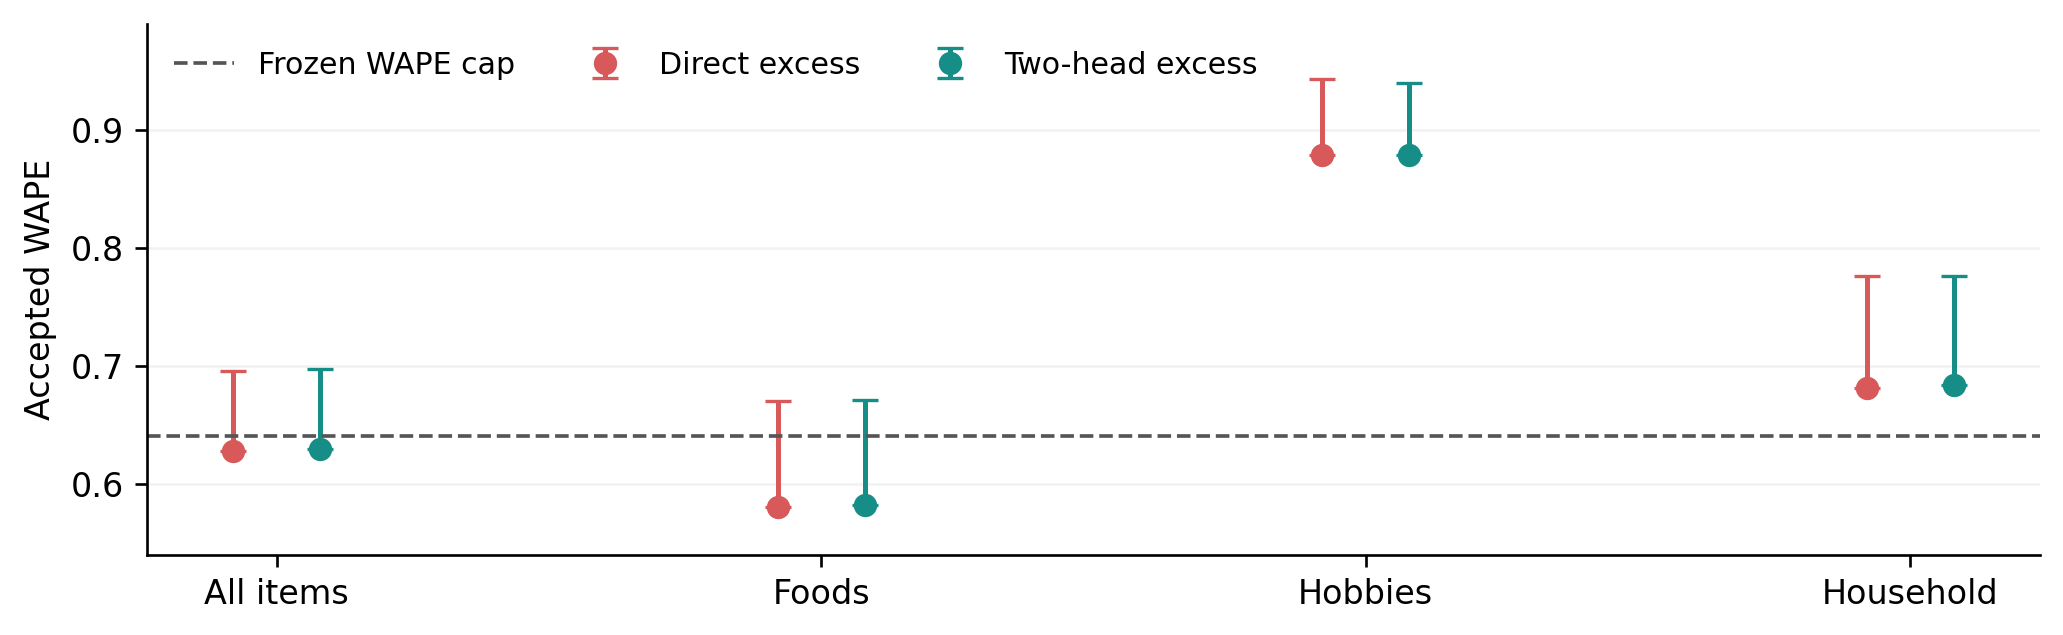
\includegraphics[width=\linewidth]{figures/guardian_groups.png}
\caption{Previously held-out items, first prespecified seed and frozen pooled thresholds. Dots are shadow WAPE; whiskers extend to the one-sided bootstrap upper bound at nominal tail probability $0.05/48$. Hobbies and Household fail the cap even at their point estimates. All displayed adjusted upper bounds exceed the cap.}
\label{fig:guardiangroups}
\end{figure}
\begin{table}[htbp]
\centering\small
\caption{Pooled endpoints from the prespecified first-seed guardian audit. Each bound uses tail probability $0.05/48$ and 10,000 item-bootstrap draws. The full 24-row, 48-endpoint record remains in the supplement; all coverage lower bounds exceed 0.35 and all WAPE upper bounds exceed 0.64013.}
\label{tab:m5guardianbounds}
\begin{tabular}{llrrrr}\toprule
Method & Period & Coverage & WAPE & Cov. lower & WAPE upper\\\midrule
Direct & A & 0.8914 & 0.6399 & 0.8745 & 0.7161\\
Direct & B & 0.8794 & 0.6495 & 0.8630 & 0.7225\\
Direct & Shadow & 0.8725 & 0.6282 & 0.8560 & 0.6959\\
Two-head & A & 0.8895 & 0.6401 & 0.8729 & 0.7160\\
Two-head & B & 0.8763 & 0.6504 & 0.8596 & 0.7236\\
Two-head & Shadow & 0.8746 & 0.6296 & 0.8587 & 0.6971\\
\bottomrule\end{tabular}
\end{table}

Across all four strata, coverage lower bounds range from 0.8040 to 0.9288 and WAPE upper bounds from 0.6704 to 0.9468. Thus every WAPE endpoint misses the cap, including Foods; this is a failure of the specified joint check, not merely the pooled rows in Table~\ref{tab:m5guardianbounds}.
A truncated derived cache was restored from unchanged models; readable arrays matched exactly, and saved masks reproduce all 504 policy/period/stratum records. Frozen results and hashes are unchanged. Subsequent objective, floor, capacity, loss, and partial-label diagnostics reuse this consumed holdout and remain exploratory.

\subsection{The separately frozen external comparison}
\label{app:external}
At 14:29 UTC on 6 September 2026, an initial pending plan froze direct excess versus demand-normalized error with floor 0.25. At 14:47 UTC, after inspecting the consumed first-holdout mixed-utility diagnostics, we replaced that pair with composed excess ($\lambda=1$) versus mixed utility ($\lambda=0.25$). No external data had been accessed under either plan. The earlier plan is preserved byte for byte; the final plan records its hash and replacement reason. The first external access was at 15:10 UTC and evaluation completed at 15:13 UTC. This is a prospectively fixed external comparison selected after first-holdout exploration, not a test independently specified before that exploration.

The final plan fixes 27 dependencies, seed 20260906, the point forecast, 220-tree heads, and development thresholds and scale. No external fit, threshold search, or scale update occurred. Exact values, timestamps, and hash-linked plan history are supplied in the reproduction package.

The 610 external items (269 Foods, 117 Hobbies, 224 Household) yield 140,300 primary rows on days 1919--1941, with every forecast origin after day 1913. Observed history through day 1913 and subsequent observations available at each origin form the features; truth is used only for evaluation. Targets 1914--1918, issued at origin 1911, enter only a prespecified 28-day descriptive sensitivity. Paired item-bootstrap draws (10,000; seed 20260906) test mixed-minus-row demand gain and row loss with one-sided 97.5\% bounds. Both must exclude zero in the specified direction. Separately, two policies, three periods (1919--1941, 1919--1929, 1930--1941), four strata, and two bounds give 48 secondary endpoints, each at tail level $0.05/48$. The primary and secondary families each use nominal 0.05; they do not form one joint 95\% claim. Item resampling retains stores and dates but not shared-shock uncertainty. Because the first holdout failed its operating requirements, this test separately asks whether the fixed coverage contrast transfers and whether the operating constraints hold.

\begin{table}[H]
\centering\small
\caption{One-time external comparison: 610 items, days 1919--1941. Two policies were fixed before opening; thresholds and heads are unchanged. Point WAPE passes the pooled cap, but the 48-endpoint operating check fails.}
\label{tab:external}
\begin{tabular}{lrrr}
\toprule
Fixed policy & Rows (\%) & Demand (\%) & WAPE\\
\midrule
Row utility, $\lambda=1$ & 85.92 & 83.19 & 0.6065 \\
Mixed utility, $\lambda=0.25$ & 82.57 & 88.35 & 0.6081 \\
\bottomrule
\end{tabular}
\par\smallskip\begin{minipage}{0.97\linewidth}\footnotesize
Only the first seed and $\lambda\in\{1,0.25\}$ were frozen for this test. The pair was selected after the first holdout; other external seeds and the full $\lambda$ grid were not evaluated. The test verifies transfer of this selected contrast.
\end{minipage}
\end{table}

\label{sec:external}\label{sec:heldout}
Mixed utility gains 5.16 demand-coverage points and loses 3.35 case points (Table~\ref{tab:external}); both prespecified directional bounds exclude zero. This confirms transfer of the selected contrast, not of the later paired-refit or five-rule menu procedures. Pooled point risks pass, but all 24 adjusted risk upper bounds exceed the cap; all 24 case-coverage lower bounds pass. Hobbies and Household violate the cap at their point estimates. The union remains point-feasible, so this external result establishes neither binding budget competition nor Pareto optimality.

\begin{table}[t]
\centering\small
\caption{All 48 external secondary bounds. Each pair is row-coverage lower bound (\%) / WAPE upper bound; each tail uses $0.05/48$. Every row bound passes 35\%; every WAPE bound fails 0.64013. The two main directional bounds are a separate family.}
\label{tab:external-bounds}
\begin{tabular}{llrr}
\toprule
Period & Stratum & $\lambda=1$ & $\lambda=0.25$\\
\midrule
All 23 days & All & 83.90 / 0.6896 & 80.81 / 0.6863 \\
 & Foods & 78.70 / 0.6634 & 76.73 / 0.6684 \\
 & Hobbies & 75.58 / 0.9171 & 76.99 / 0.8864 \\
 & Household & 91.57 / 0.7813 & 84.64 / 0.7618 \\
First 11 days & All & 83.10 / 0.6908 & 80.56 / 0.6896 \\
 & Foods & 77.30 / 0.6637 & 76.12 / 0.6727 \\
 & Hobbies & 75.72 / 0.9161 & 77.02 / 0.8803 \\
 & Household & 90.98 / 0.7824 & 84.51 / 0.7642 \\
Last 12 days & All & 84.48 / 0.6907 & 81.00 / 0.6860 \\
 & Foods & 79.78 / 0.6658 & 77.08 / 0.6643 \\
 & Hobbies & 75.55 / 0.9201 & 76.84 / 0.8937 \\
 & Household & 91.99 / 0.7791 & 84.62 / 0.7637 \\
\bottomrule
\end{tabular}
\end{table}

The full-28-day sensitivity has row/demand coverage 86.14\%/82.87\% for $\lambda=1$ and 82.51\%/87.94\% for $\lambda=0.25$, with WAPE 0.6128/0.6133. It is descriptive only. The archived execution has one opening, zero fits, and zero threshold searches; saved item-level accepted counts, error sums, and demand sums reproduce the primary bounds and all 48 secondary endpoints.

\paragraph{Descriptive external budget accounting.}
We apply equation~\eqref{eq:budget} retrospectively to the same saved masks (Table~\ref{tab:externalbudget}). Row-only and mixed-only sets spend 30.20\% and 29.45\% of common slack, yet contain 3.32\% and 8.48\% of demand. Both retain slack; the joint operating failure remains. This adds no confirmatory endpoint, fit, threshold, or policy; the superseded pair is not evaluated.
\begin{table}[t]
\centering\small
\caption{Descriptive budget accounting for the two frozen external policies, days 1919--1941. $K$ is their intersection; $U$ is accepted only at $\lambda=1$, and $V$ only at $\lambda=0.25$. Demand shares use the total 209,893 units. Signed excess is $E_B-rM_B$; a negative value supplies slack. This analysis reuses saved predictions after the confirmation result.}
\label{tab:externalbudget}
\begin{tabular}{lrrrrr}
\toprule
Set & Rows & Demand (\%) & WAPE & Mean $f$ & Excess \\
\midrule
Common $K$ & 109,985 & 79.86 & 0.5899 & 1.112 & -8,421.10 \\
Row-only $U$ & 10,557 & 3.32 & 1.0046 & 0.122 & 2,542.83 \\
Mixed-only $V$ & 5,855 & 8.48 & 0.7794 & 1.703 & 2,480.43 \\
\bottomrule
\end{tabular}
\end{table}


\subsection{Retained historical controls and reproduction}
\label{app:history}\label{app:legacyselection}
The numerical supplement retains the earlier weak-forecast controls and all seed/category/period reports. The prior FreshRetailNet check used observable evaluation labels, not hidden stockout demand: shadow row coverage/WAPE 0.28163/0.30484 missed both 0.30 targets, with adjusted bounds 0.25713/0.31821. Calibration B's coverage lower bound was 0.28498. This failed check supplies no natural-stockout confirmation.

The notebook checks frozen hashes before and after replaying theory, moments, and external sufficient statistics. All verification output goes to a separate directory. Experiment scripts regenerate fits from public M5. The separate numerical assets include the derived development inputs needed for the new predictor-specific selector replay; original external replay uses retained sufficient statistics.

\section{Objective choice and supervised-head diagnostics}
\label{app:objective}
\begin{table}[t]
\centering\small
\caption{Strong fixed forecaster; three matched risk-training seeds. Values are development-shadow means $\pm$ training-seed SD (not independent-test uncertainty). Thresholds use the same two calibration blocks and row-coverage objective. Numbers in parentheses denote total boosting trees. The two-head budget-220 control uses 110 trees per head.}
\label{tab:twohead}
\begin{tabular}{lrrr}\toprule
Score & Row coverage (\%) & Demand coverage (\%) & WAPE\\\midrule
Forecast-normalized & 80.22 $\pm$ 0.27 & 86.58 $\pm$ 0.09 & 0.6216 \\
Demand-normalized & 74.17 $\pm$ 0.85 & 89.01 $\pm$ 0.20 & 0.6260 \\
Forecast excess & 81.47 $\pm$ 0.41 & 70.71 $\pm$ 0.59 & 0.6222 \\
Two-head excess (440) & 86.35 $\pm$ 0.08 & 81.32 $\pm$ 0.21 & 0.6268 \\
Two-head excess (220) & 86.61 $\pm$ 0.12 & 81.88 $\pm$ 0.29 & 0.6269 \\
Direct excess (220) & 86.30 $\pm$ 0.16 & 80.86 $\pm$ 0.11 & 0.6245 \\
\bottomrule\end{tabular}
\end{table}

\begin{table}[t]
\centering\small
\caption{Explicit objective-based family selection among the seven original scores, followed by threshold application to shadow periods. Three-seed means. Both objectives retain WAPE cap 0.64013 and row floor 0.35 in calibration A/B. Guardian rows are post-hoc reuse of the same consumed holdout, not new confirmation.}
\label{tab:objectives}
\begin{tabular}{lllrrr}\toprule
Cohort & Objective & Selected score & Rows (\%) & Demand (\%) & WAPE\\\midrule
Design & Row & Direct excess (220) & 86.30 & 80.86 & 0.6245 \\
Guardian & Row & Direct excess (220) & 87.37 & 83.29 & 0.6280 \\
Design & Demand & Demand-normalized & 74.17 & 89.01 & 0.6260 \\
Guardian & Demand & Demand-normalized & 73.62 & 88.23 & 0.6219 \\
\bottomrule\end{tabular}
\end{table}

\subsection{Architecture controls and first-holdout detail}
\label{app:architecture}
\paragraph{Development accepted-set accounting.}
Direct excess gains 6.08 percentage points in mean row coverage over forecast-normalized error, but loses 5.71 points of demand coverage. At the first seed, their common accepted set covers 73.35\% of rows and has WAPE 0.5958, leaving slack under the 0.64013 cap. The direct-only set adds 267,656 rows (12.84\% of all rows), but only 5.69\% of demand; its WAPE is 1.0026. The relative-only set contains 141,617 rows and 11.45\% of demand, with WAPE 0.7915. Mean forecasts in the two differing sets are 0.039 and 1.498 units. In equation~\eqref{eq:budget}, the common set supplies 97,185.97 units of excess slack. The direct-only set consumes 60,141.11 (61.88\%), versus 50,549.56 (52.01\%) for the relative-only set. Both fit within the pooled budget despite their individual WAPE exceeding the cap. This accounts for the row gain through budget use and demand composition.


\paragraph{Architecture is distinct from acceptance utility.}
The original matched selector comparison provides an architectural control. Direct-excess, two-head, and matched-tree-budget two-head scores reach 86.30\%, 86.35\%, and 86.61\% mean row coverage. Direct learning has slightly lower accepted WAPE (0.6245 versus 0.6268 and 0.6269); it does not establish a direct-learning advantage. The informative distinction is the coverage objective and resulting budget allocation, not whether excess is learned directly or composed from two heads. Full three-seed results are in Appendix~\ref{app:objective}.

\subsection{Detailed first item-holdout comparison}
\label{app:architecture-holdout}
\begin{table}[t]
\centering\small
\caption{Previously held-out M5 items: fixed pooled thresholds, 610 items, 6,100 series, and 695,400 shadow rows. Three-seed means; all fits and thresholds were frozen before opening. Seeds measure training variability, not three independent holdouts. Absolute-error selection accepts no rows and has undefined WAPE.}
\label{tab:m5guardian}
\begin{tabular}{lrrr}\toprule
Score & Row coverage (\%) & Demand coverage (\%) & WAPE\\\midrule
Forecast-normalized & 80.87 & 87.65 & 0.6219 \\
Demand-normalized & 73.62 & 88.23 & 0.6219 \\
Forecast excess & 82.74 & 74.59 & 0.6251 \\
Two-head excess (440) & 87.41 & 83.69 & 0.6297 \\
Two-head excess (220) & 87.67 & 84.18 & 0.6297 \\
Direct excess (220) & 87.37 & 83.29 & 0.6280 \\
\bottomrule\end{tabular}
\end{table}

The freeze specifies seven scores, two threshold modes, three seeds, and a first-seed direct-versus-two-head primary contrast. The holdout uses the same A/B and later evaluation dates, without recalibration; no holdout outcome selects an original policy. Its shadow contains 695,400 rows on days 1800--1913.

The coverage trade-off persists (Table~\ref{tab:m5guardian}). Across three fixed fits, direct excess increases row coverage by 6.49 percentage points over forecast-normalized error while reducing demand coverage by 4.36 points. Two-head coverage is 87.41\%, compared with 87.37\% for direct learning, with WAPE 0.6297 versus 0.6280. At the prespecified first seed, direct minus two-head row coverage is $-0.215$ points (paired 95\% item-bootstrap interval $[-0.413,-0.018]$ points); direct WAPE is lower by 0.00141. These are different trade-offs, not an equivalence result or a direct-learning advantage.



Operating constraints do not transfer jointly. First-seed direct and two-head shadow WAPE are 0.6282 and 0.6296 pooled, but approximately 0.879 for Hobbies and 0.682--0.683 for Household. In the holdout window matching calibration B, even pooled WAPE is 0.6495 and 0.6504, above the 0.64013 cap. All frozen category-specific policies abstain entirely on Hobbies because their development threshold is absent. The prespecified 48-endpoint family covers two primary methods, three periods, four strata, and two bounds, using 10,000 item-bootstrap draws. Every coverage lower bound exceeds 0.35, but every adjusted WAPE upper bound exceeds the cap; shadow pooled upper bounds are 0.6959 and 0.6971. This fails the specified joint operating check. Appendix~\ref{app:heldout} reports all bounds and the access record.


\begin{figure}[t]
\centering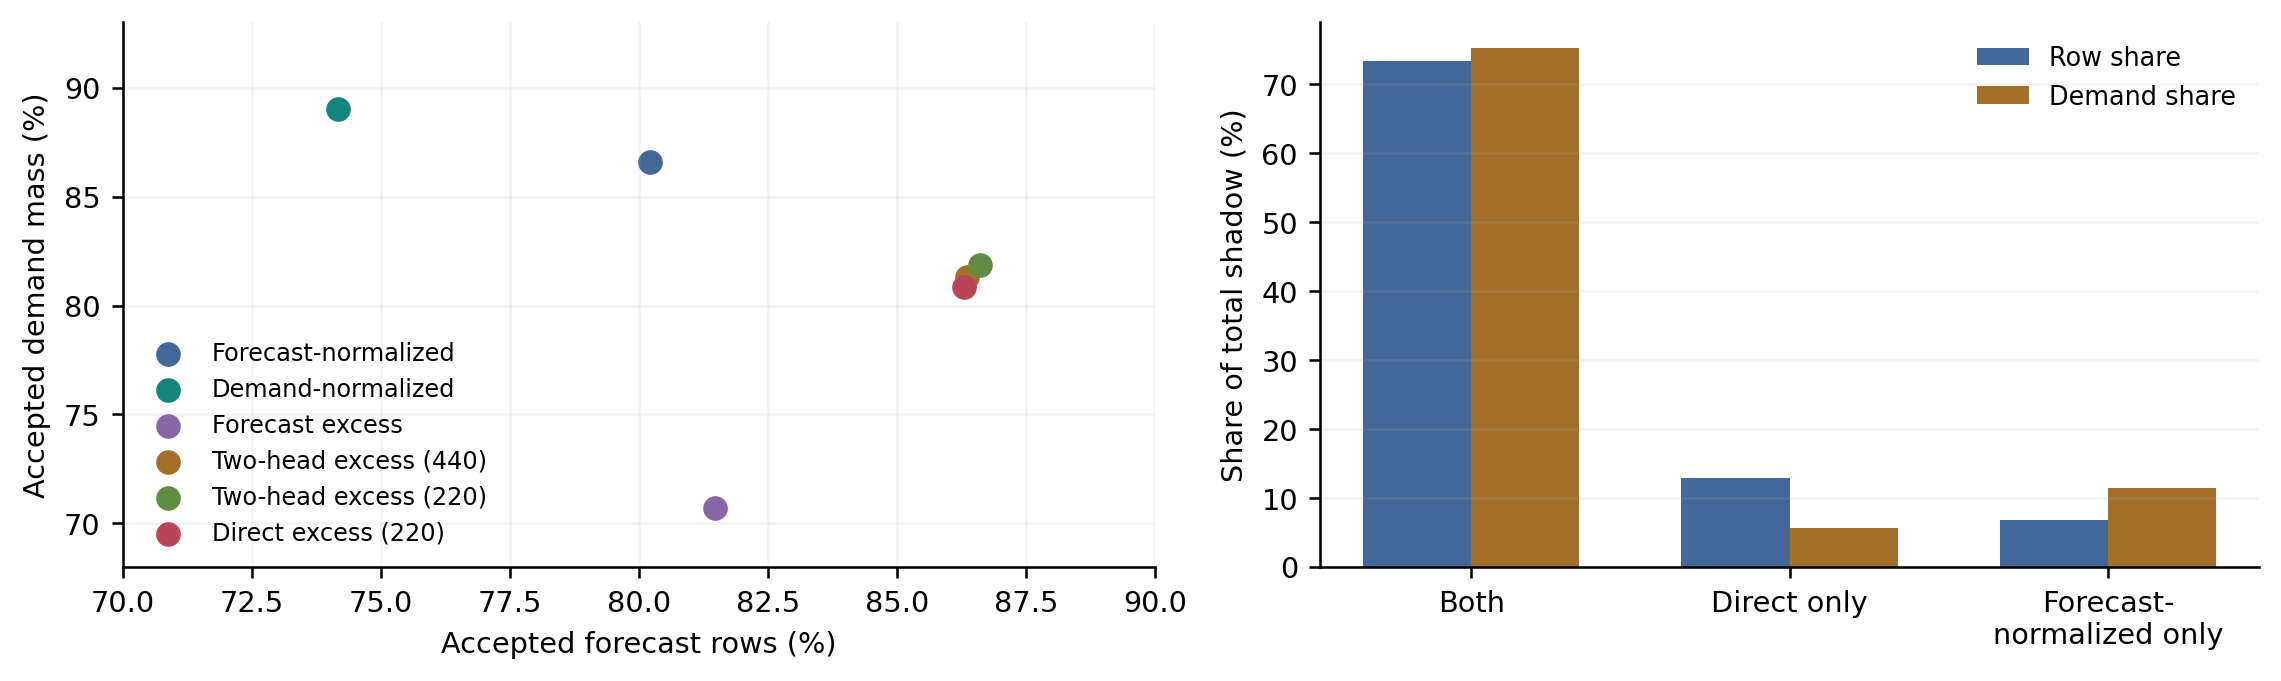
\includegraphics[width=\linewidth]{figures/row_vs_demand.png}
\caption{Original development comparison. Left: three-seed means under row-coverage threshold selection. Right: first-seed direct-excess and forecast-normalized-error acceptance sets. The direct-only set has more cases and less demand. These previously evaluated results precede the additional menu audit.}
\label{fig:mass}
\end{figure}


\subsection{Nested paths, family choice, and denominator regularization}
For a fixed score, $A_t=\{s\leq t\}$ is nested. Both $P(A_t)$ and $\E[Y\ind_{A_t}]/\E Y$, including their empirical blockwise minima, are nondecreasing in $t$. WAPE need not be monotone, but the largest member of any nonempty finite feasible grid maximizes either coverage. An empty grid returns no policy.

Across 27 score/seed pairs (nine rankings, three fits), changing only the coverage objective leaves all thresholds unchanged: 24 finite and three infeasible. Family choice instead selects direct excess for rows and demand normalization for demand. The later audit uses the largest maximizer, changing 1--3 shadow rows in four configurations relative to the original first-maximizer convention; frozen results are preserved.

\texttt{CAP\_REFERENCE.json} reproduces the legacy development-selection WAPE 0.7530939208313988 and the archived cap $r=.85\times.7530939208313988$. Table~\ref{tab:floors} varies the unit-sales denominator regularizer without guardian-based selection. Demand normalization wins the family comparison at floor 0.25; the smaller-floor reversals limit any claim about estimated $e/\mu$.
\begin{table}[htbp]
\centering\small
\caption{First-seed denominator-floor sensitivity on consumed guardian shadow. F/D denote forecast/demand normalization. Thresholds use development A/B; no floor is selected on guardian. Full development metrics remain in the numerical supplement.}
\label{tab:floors}
\begin{tabular}{rrrrr}\toprule
Floor & F demand (\%) & D demand (\%) & F WAPE & D WAPE\\\midrule
0 & 87.77 & 87.53 & 0.6195 & 0.6186\\
0.01 & 87.75 & 87.53 & 0.6193 & 0.6186\\
0.05 & 87.97 & 87.53 & 0.6201 & 0.6186\\
0.1 & 87.98 & 87.58 & 0.6206 & 0.6188\\
0.25 & 87.73 & 88.10 & 0.6219 & 0.6211\\
0.5 & 85.53 & 89.11 & 0.6249 & 0.6257\\
1 & 74.47 & 86.32 & 0.6286 & 0.6297\\
\bottomrule\end{tabular}
\end{table}


\subsection{Mixed utility and the zero-floor comparison}
\label{app:mixed}
For a nonbinding row floor, $w_\lambda=\lambda+(1-\lambda)\mu/T$ defines a probability measure since $\E w_\lambda=1$. At fixed $U_\lambda=\E[aw_\lambda]$, the exchange proof orders $m_r/w_\lambda$ and minimizes excess. Largest feasible weighted prefixes maximize that utility; boundary randomization handles ties. At $\lambda=0$, reject $\mu=0,e>0$ without losing utility; zero-error/zero-demand contexts are neutral. With a binding row floor, a finite-policy LP has Lagrangian coefficient $w_\lambda+\zeta-\tau m_r$, $\zeta\geq0$. If $\tau>0$, its score is $m_r/(w_\lambda+\zeta)$, with $\zeta(c-c_0)=0$. Thus the simple score alone need not solve a binding-floor problem.

The exploratory grid uses first-seed 220-tree heads, zero-clipping, and development A/B mean demand $\hat T$. A/B outcomes alone select thresholds. All five guardian policies are reported; each fails period-B pooled WAPE. At $\lambda=0$, positive-error/zero-demand rows rank last and $0/0$ is zero. The mixed $\lambda=0.25$ point exceeds $\lambda=0$ in both coverages; imperfect fitted heads permit this empirical dominance.
\begin{table}[htbp]\centering\small
\caption{Fixed mixed-utility grid on consumed guardian predictions (one predeclared fit). All choices are made on development A/B; no guardian-best mixture is selected.}
\label{tab:mixed}
\begin{tabular}{rrrrr}\toprule
$\lambda$ & Shadow rows (\%) & Shadow demand (\%) & Shadow WAPE & B WAPE\\\midrule
0 & 62.74 & 87.53 & 0.6186 & 0.6428\\
0.25 & 84.31 & 88.67 & 0.6272 & 0.6467\\
0.5 & 86.42 & 87.87 & 0.6287 & 0.6473\\
0.75 & 87.28 & 86.24 & 0.6292 & 0.6488\\
1 & 87.46 & 83.78 & 0.6296 & 0.6504\\
\bottomrule\end{tabular}\end{table}

\begin{table}[htbp]
\centering\small\setlength{\tabcolsep}{3.2pt}
\caption{Development mixed-utility path before item transfer. One common A/B-selected threshold per $\lambda$; first-seed heads. Coverages are percentages. All A/B pooled point constraints pass; these reused calibration outcomes give no independent risk guarantee.}
\label{tab:mixed-development}
\begin{tabular}{r rrr rrr rrr}\toprule
&\multicolumn{3}{c}{Calibration A}&\multicolumn{3}{c}{Calibration B}&\multicolumn{3}{c}{Later evaluation}\\
$\lambda$&Rows&Demand&WAPE&Rows&Demand&WAPE&Rows&Demand&WAPE\\\midrule
0 & 71.68 & 89.85 & 0.6401 & 67.45 & 88.45 & 0.6381 & 64.22 & 88.43 & 0.6231\\
0.25 & 85.25 & 88.67 & 0.6396 & 84.06 & 87.97 & 0.6401 & 83.77 & 88.54 & 0.6278\\
0.5 & 86.71 & 86.91 & 0.6388 & 85.69 & 86.57 & 0.6401 & 85.63 & 87.02 & 0.6278\\
0.75 & 87.54 & 84.68 & 0.6387 & 86.46 & 84.45 & 0.6401 & 86.36 & 84.68 & 0.6277\\
1 & 87.83 & 81.56 & 0.6390 & 86.63 & 81.46 & 0.6401 & 86.42 & 81.56 & 0.6275\\
\bottomrule\end{tabular}
\end{table}

Without a positive floor, forecast-normalized guardian row/demand coverage is 44.62\%/87.77\% (WAPE 0.6195), versus demand-normalized 62.74\%/87.53\% (0.6186). The latter masks equal the $\lambda=0$ endpoint, as required by their affine score relationship.

\subsection{Error-head bottleneck and finite-capacity effects}
\begin{table}[htbp]
\centering\small
\caption{Hobbies outcome substitutions, first seed. Each path optimizes its own later-window threshold, using realized labels in the excess score. Coverages are percentages; dashes mean no feasible prefix. These are samplewise diagnostics, not deployable conditional-mean oracles.}
\label{tab:partialoracles}
\begin{tabular}{lrrr rrr}\toprule
&\multicolumn{3}{c}{Development}&\multicolumn{3}{c}{Item holdout}\\
Replaced head&Rows&Demand&WAPE&Rows&Demand&WAPE\\\midrule
Neither&0.00&0.00&--&0.00&0.00&--\\
Error only&76.78&23.90&0.6401&76.38&21.28&0.6401\\
Demand only&0.00&0.00&--&0.00&0.00&--\\
Both&89.15&60.94&0.6401&86.97&54.04&0.6401\\
\bottomrule\end{tabular}
\end{table}

The outcome-substitution diagnostic (Table~\ref{tab:partialoracles}) localizes a samplewise error-information gap. Positive-error/zero-demand rows rank last; zero-error/zero-demand rows cost no excess. Realized-label access includes irreducible noise and is not a conditional-learning guarantee.

Three 220-tree error-head interventions hold the point forecast and demand head fixed. Two Hobbies specialists share 107,384 rows from the original sample; their 21-versus-29-feature contrast holds the training population fixed. A new shared 29-feature head uses exactly the original 600,000 rows, resolving sample-size confounding for feature addition relative to the shared 21-feature head. Added features are positive-day count, positive-size mean/CV$^2$, and recency over 56/112 days ending at the origin. Protocols precede fitting; shared sample indices, the Hobbies subset, and original forecasts reproduce bit for bit. Future perturbations leave features unchanged. The shared 29-feature head improves both reported MSEs but yields no feasible A/B threshold or later-block prefix (Table~\ref{tab:hobbies_intervention}). Training still uses pre-censoring error labels; no new head is evaluated on either holdout. No matched Hobbies point-forecast intervention is available, so attribution to the point model remains unresolved.
\begin{table}[t]
\caption{Development Hobbies interventions, first seed. The two shared heads use the same 600,000 rows; the two specialists use the same 107,384 Hobbies rows. All use 220 trees, the same point forecast and demand head. MSE uses the later development block. No common A/B threshold, or outcome-informed later-block prefix, meets the cap and 35\% row floor. Empty-policy WAPE is undefined.}
\label{tab:hobbies_intervention}
\centering
\small
\setlength{\tabcolsep}{3pt}
\begin{tabular}{lrrrrrr}
\toprule
Error head & Train rows & MSE & Positive MSE & Rows (\%) & WAPE & Prefix (\%) \\
\midrule
Shared, 21 features & 600,000 & 2.3554 & 7.8403 & 0.00 & -- & 0.00 \\
Shared, 29 features & 600,000 & 2.3370 & 7.7650 & 0.00 & -- & 0.00 \\
Hobbies, 21 features & 107,384 & 2.4232 & 7.9048 & 0.00 & -- & 0.00 \\
Hobbies, 29 features & 107,384 & 2.4399 & 7.9392 & 0.00 & -- & 0.00 \\
\bottomrule
\end{tabular}
\end{table}

Capacity controls show that enlarging only the error head lowers held-out row coverage by 0.45--0.63 points, whereas enlarging only demand raises it by 0.20--0.38 points and raises WAPE. Both heads together increase excess MSE from 1.0630 to 1.0868. The numerical supplement retains all 288 error/demand/cross-moment decompositions.

\subsection{Demand-head loss controls}
Squared, Poisson, and Tweedie losses target the conditional mean under their respective moment assumptions; the supplement gives the derivatives. Six matched 220-tree Poisson/Tweedie ($p=1.5$) demand heads improve held-out demand coverage, but period-B WAPE remains 0.6470/0.6467. Full seed results are archived.

\subsection{Group-budget control in a fixed learned-score class}
\label{app:grouplp}
For each category, predicted error and demand from the first-seed 220-tree heads define an $8\times8$ quantile grid using development A/B scores only. Bin probabilities $z_j\in[0,1]$ are shared across both blocks. The LP maximizes minimum block row coverage, enforcing $\sum_j z_j(E_{gjb}-rM_{gjb})\leq0$ and $\sum_jz_jN_{gjb}\geq0.35N_{gb}$ separately for each group $g$ and block $b$. No category borrows another's budget. Calibration outcomes determine the probabilities; bins, coefficients, and probabilities are fixed before application to the consumed guardian. These are exploratory point constraints, not independent calibration bounds.

All 28 occupied Hobbies bins in A and 29 in B have positive excess. Their minimum WAPE is 0.7289866 and 0.7503685, respectively, so every nonempty fractional mixture has WAPE above the cap in either block. At the row floor, a dual certificate bounds the minimum worst-block mean excess below by 0.0142589987 units per original row. The supplement supplies coefficients and a verifier checking residual-corrected dual bounds. This infeasibility concerns the specified grid, not arbitrary features or acceptance rules.

Foods and Household attain minimum calibration row coverage 94.60\% and 76.76\%. Their transferred guardian B WAPE is 0.6392 and 0.6459; shadow WAPE is 0.6111 and 0.6455. Thus the group constraints expose Hobbies failure and retain Household transfer failure. Fractional metrics are ratios of expected accepted sums; a realized randomized deployment can fluctuate around them.

\section{Observed-sales and capacity likelihood controls}
\label{app:observable}
\begin{table}[t]
\centering\small\setlength{\tabcolsep}{3pt}
\caption{First-seed NB grid on development data. A/B/shadow pairs are implied / realized WAPE; rows are shadow coverage. The star selects observed validation NLL among $\{1,1.5,2,3,5\}$; 0.5/10 are descriptive anchors. Intervals are $10^{-3}$ NLL differences from shape 2, with four-comparison Bonferroni adjustment using 10,000 paired item-bootstrap draws. They reuse the selection data and condition on fitted models. Dashes in risk columns mean no admissible threshold.}
\label{tab:nb-fine-grid}
\begin{tabular}{rrrrrrr}
\toprule
$\kappa$ & Valid. NLL & $\Delta$NLL interval & Calibration A & Calibration B & Shadow & Rows (\%)\\
\midrule
0.5 & 0.7541 & -- & -- / -- & -- / -- & -- / -- & 0.00 \\
1 & 0.7361 & [2.934, 6.334] & -- / -- & -- / -- & -- / -- & 0.00 \\
1.5 & 0.7324 & [0.220, 1.634] & -- / -- & -- / -- & -- / -- & 0.00 \\
2 * & 0.7314 & reference & 0.6401 / 0.5597 & 0.6376 / 0.5578 & 0.6365 / 0.5484 & 48.74 \\
3 & 0.7322 & [-0.008, 1.592] & 0.6401 / 0.6421 & 0.6368 / 0.6412 & 0.6355 / 0.6311 & 79.48 \\
5 & 0.7347 & [1.606, 5.031] & 0.6401 / 0.6861 & 0.6361 / 0.6856 & 0.6334 / 0.6748 & 99.41 \\
10 & 0.7392 & -- & 0.6076 / 0.6902 & 0.6033 / 0.6888 & 0.5997 / 0.6790 & 100.00 \\
\bottomrule
\end{tabular}
\end{table}

\subsection{Observation model and available information}
This development-only experiment keeps the plain observed-sales L1 forecast fixed; forecast choice and the cap inherit outcome-informed development history. The strict benchmark flag $\Delta=\ind\{Y>C\}$ differs from the observable capacity hit $H=\ind\{S\geq C\}$, which reveals only $Y\geq C$. The capacity branch uses $H$ in both responses and historical features. Each fit samples 600,000 risk rows from days 1436--1532, validates on 1534--1553, and uses 34 origin-valid inputs, 220 trees, 31 leaves, and the common training settings. Three seeds are retained; shape selection uses observed-data validation likelihood.

Let $p_\theta(y\mid X)$ be Poisson with mean $\mu_\theta$, or NB with mean $\mu_\theta$ and fixed shape $\kappa$ (variance $\mu_\theta+\mu_\theta^2/\kappa$). The two negative log likelihoods are
\begin{align*}
 \ell_\Delta&=-(1-\Delta)\log p_\theta(S\mid X)-\Delta\log\Pr_\theta(Y>C\mid X),\\
 \ell_H&=-(1-H)\log p_\theta(S\mid X)-H\log\Pr_\theta(Y\geq C\mid X).
\end{align*}
For integer counts, the latter survival is evaluated at $C-1$. These likelihoods require an appropriate conditional count family and ignorable censoring given modeled information. Dependence of capacity on past sales does not automatically justify ignorability for a finite feature vector. The method therefore models the hidden tail; it does not nonparametrically identify it.

\subsection{Implied moments, thresholding, and results}
For $k=\lfloor f\rfloor$ and nonnegative $f$, the distribution implies
\[
 \hat e=\E_\theta|Y-f|=\hat\mu-f+2\{fF_\theta(k)-\E_\theta[Y\ind\{Y\leq k\}]\}.
\]
The truncated moment is $\hat\mu F_{\operatorname{Pois}(\hat\mu)}(k-1)$ for Poisson and $\hat\mu F_{\operatorname{NB}(\kappa+1,p)}(k-1)$ for NB, with $p=\kappa/(\kappa+\hat\mu)$. Direct summation and finite differences check moments and likelihood derivatives, including extreme tails.

A/B thresholds maximize common row coverage under $\sum a\hat e/\sum a\hat\mu\leq r$ and the 0.35 floor. Both excess and demand-normalized rankings are archived. Implied and realized risk differ through
\[
 R(a)-r=\frac{\E[a(\hat e-r\hat\mu)]+\E[a(e-\hat e)]-r\E[a(\mu-\hat\mu)]}{\E[a\mu]}.
\]
Hence passing the implied constraint is not an observed-risk certificate. Table~\ref{tab:observablemoments} reports both numerator/denominator pairs.

\begin{table}[t]
\centering\small
\caption{Sales-and-capacity NB $\kappa=2$ at its observed-likelihood-selected, model-implied threshold. Bias is $(\widehat E/E-1)$ or $(\widehat M/M-1)$ on the same accepted rows. Each entry averages three fit-specific ratios. Positive error-mass bias exceeds positive demand-mass bias, making the implied ratio conservative in aggregate.}
\label{tab:observablemoments}
\begin{tabular}{lrrrrr}
\toprule
Period & Rows (\%) & Implied WAPE & Realized WAPE & Error bias (\%) & Demand bias (\%)\\
\midrule
A & 49.96 & 0.6401 & 0.5568 & +18.82 & +3.35\\
B & 49.44 & 0.6376 & 0.5562 & +21.65 & +6.12\\
Shadow & 48.17 & 0.6365 & 0.5461 & +20.59 & +3.46\\
\bottomrule\end{tabular}\end{table}

Across three fits per observation branch, validation selects $\kappa=2$; Hobbies WAPE remains 0.8018. All 33 retained fits and seven derivative, moment, origin, and equality tests are archived.

\FloatBarrier
\subsection{Fine dispersion grid and identical-forecast comparison}
All fine-grid fits share the sample, features, and forecast; protocols and hashes precede fitting. The count-matched supervised head uses the same inputs and a realized-excess target. Outcome-independent boundary draws agree with fractional-tie expectations (264 records and 21 count matches verified). Uniform fractional abstention at 48.17\% instead has equal demand coverage and WAPE 0.6790.

\paragraph{Validation likelihood uncertainty.}
All seven observed NLL means reproduce exactly. The 10,000 paired-bootstrap draws resample 1,829 validation items (365,800 rows), retaining each item's stores and dates. The four adjusted comparisons use two-sided tails $0.05/(2\times4)$; pointwise 95\% intervals are all positive. These approximate intervals reuse the data that selected shape 2 and condition on fitted models; they neither confirm the selected winner independently nor identify censored tails. Shared store/calendar shocks remain unaccounted for. Saved item sums reproduce all intervals without fitting.

\subsection{Observed-data diagnostics and their target population}
\label{app:natural-diagnostics}
Theoretical selection uses conditional loss and exposure; naturally hidden demand does not supply either without assumptions. Our observed-sales-and-capacity negative-binomial experiment illustrates the issue. Among adjusted paired item-bootstrap comparisons, shape $\kappa=3$ is the only candidate whose validation likelihood difference from selected $\kappa=2$ includes zero, yet it breaks both realized calibration caps that $\kappa=2$ passes. The selected model overestimates aggregate error mass by 20.59\%; its pooled point pass does not validate conditional moments. Appendix~\ref{app:observable} provides the likelihood, dispersion grid, and count-matched supervised control.

Further forecasting experiments on naturally stockout-annotated FreshRetailNet test observable sales outcomes, not hidden demand. A forward-time residual learner reduces WAPE on the 8,020 non-stockout test rows from 0.32928 to 0.29201, and on all 14,000 recorded-sales rows from 0.36162 to 0.33401. These later comparisons reuse the previously opened seven-day cohort; most improvement remains without the risk feature (non-stockout WAPE 0.29289). They demonstrate useful forecast adaptation within that evaluated population, but cannot certify an acceptance constraint for demand coverage on unobserved stockout demand. Appendix~\ref{app:accuracy} records the controls and uncertainty. Thus accuracy improvement, acceptance utility, and identification are three distinct requirements of a forecasting engine.



\section{Accuracy improvement with newly fitted acceptance policies}
\label{app:accuracy}
\subsection{A distinct retrospective protocol}
The additional experiment uses only the 1,829 development items and origin-valid observations; neither historical holdout is accessed. All dates have been consumed in prior research. A protocol records the predictor identities, chronological blocks, head specification, utility grid, cap, floor, and bootstrap before the additional head fits. This order makes the computation auditable; it does not erase previous knowledge of evaluation performance.

The group-scaled predictor is the first hierarchy-feature XGBoost L1 fit from the forecasting experiments, trained on observed sales with 33 origin-valid features and seven cross-store item summaries. A separately learned observable capacity-hit probability $q$ is available. The residual predictor is
\[
 f_{\rm res}(X)=\max\{f_0(X)+g(X,f_0(X),q(X)),0\},
\]
where $g$ is L1 gradient boosting trained on retained-target residuals. Days 1314--1373 fit candidate corrections and 1374--1433 select depth in $\{2,4\}$ and tree count in $\{50,150,300\}$; parent scaling is a fallback. Learning rate is 0.03 and minimum leaf sample size is 50. The selected depth-4, 300-tree correction is refitted on their union (up to 400,000 sampled rows). No accuracy parameter is retuned during the new selector comparison. The correction is conventional residual learning, not a proposed architecture.

Chronos-2 uses the archived univariate, nonnegative median forecasts, context up to 2,048, horizon seven, and no cross-series learning. Weight revision, weight hashes, and prediction receipts accompany the data. Raw backbone outputs are used; the older risk-bin recalibration, which was fitted on an overlapping block, is deliberately not used in this comparison. Foundation pretraining and task-specific supervised forecasting have different information histories; the within-predictor utility contrasts are the target.

The new demand head sees 40 history/hierarchy features and $q$. Each predictor-specific error head also sees that predictor's forecast. Heads use squared loss, 220 trees, 31 leaves, learning rate 0.05, minimum leaf size 50, deterministic four-thread fitting, and seed 20260908. The same 600,000 sampled training rows supply $Y$ to the demand head and $|Y-f|$ to each error head. Both outputs are clipped to nonnegative values. Thus the acceptance experiment intentionally uses benchmark truth labels; it is not an observed-sales-only solution for naturally hidden demand.

The earliest calibration origin is 1610, after all head-training targets through 1610 have been observed. The two blocks contain 35 and 28 target days; evaluation contains 114 target days with origins at least 1799. The training sample's mean demand estimates $T$. For each $\lambda\in\{1,0.25,0\}$, all distinct finite score thresholds are searched, whole ties are retained, and the largest threshold meeting pooled WAPE and row-floor constraints in both blocks is fixed. No test outcome selects a threshold or utility weight. An infeasible search would return full abstention; all nine searches are feasible. The cap uses the displayed reference $0.85\times0.7530939208$, differing from the historical full-precision cap by less than $3\times10^{-11}$.

\begin{table}[htbp]\centering\small
\caption{New within-predictor contrasts versus $\lambda=1$, in percentage points. Marginal 95\% paired item-bootstrap intervals condition on the fits and research history; 4,000 draws, 1,829 items. The pure-demand endpoint $\lambda=0$ is included without a denominator floor.}
\label{tab:accuracy-ci}
\begin{tabular}{lrrrrr}\toprule
Predictor & $\lambda$ & $\Delta$ rows & Interval & $\Delta$ demand & Interval\\\midrule
Group-scaled L1 & 0.25 & -5.77 & $[-6.45,-5.05]$ & +5.47 & $[4.34,6.64]$ \\
Group-scaled L1 & 0 & -24.07 & $[-25.50,-22.62]$ & +6.70 & $[4.92,8.53]$ \\
Residual L1 & 0.25 & -3.02 & $[-3.57,-2.43]$ & +5.87 & $[4.84,6.88]$ \\
Residual L1 & 0 & -16.87 & $[-18.07,-15.61]$ & +7.36 & $[5.78,8.94]$ \\
Chronos-2 (raw) & 0.25 & -5.35 & $[-5.96,-4.69]$ & +6.39 & $[5.45,7.31]$ \\
Chronos-2 (raw) & 0 & -22.95 & $[-24.38,-21.50]$ & +8.18 & $[6.74,9.60]$ \\\bottomrule\end{tabular}\end{table}
\begin{table}[htbp]\centering\small
\caption{Calibration pooled and later category WAPE for the new predictors. The cap is 0.64013. All nine policies meet both calibration point constraints; Hobbies and Household miss the later cap.}
\label{tab:accuracy-groups}
\begin{tabular}{lrrrrr}\toprule
Predictor & $\lambda$ & Cal. A/B & Foods & Hobbies & Household\\\midrule
Group-scaled L1 & 1 & 0.6401/0.6259 & 0.5902 & 0.8468 & 0.6839 \\
Group-scaled L1 & 0.25 & 0.6401/0.6228 & 0.5903 & 0.8321 & 0.6753 \\
Group-scaled L1 & 0 & 0.6401/0.6215 & 0.5966 & 0.8135 & 0.6612 \\
Residual L1 & 1 & 0.6401/0.6252 & 0.5901 & 0.8518 & 0.6855 \\
Residual L1 & 0.25 & 0.6401/0.6232 & 0.5894 & 0.8366 & 0.6785 \\
Residual L1 & 0 & 0.6401/0.6233 & 0.5940 & 0.8295 & 0.6699 \\
Chronos-2 (raw) & 1 & 0.6401/0.6301 & 0.5909 & 0.8520 & 0.6870 \\
Chronos-2 (raw) & 0.25 & 0.6401/0.6259 & 0.5898 & 0.8354 & 0.6744 \\
Chronos-2 (raw) & 0 & 0.6401/0.6251 & 0.5967 & 0.8164 & 0.6603 \\\bottomrule\end{tabular}\end{table}
\begin{table}[htbp]\centering\small
\caption{Budget decomposition for $\lambda=1$ versus $\lambda=0.25$ in the new retrospective comparison. Demand share uses the whole evaluation denominator; excess is absolute-error mass minus $r$ times demand mass. Negative common excess supplies slack.}
\label{tab:accuracy-budget}
\begin{tabular}{llrrrrr}\toprule
Predictor & Set & Rows & Demand (\%) & WAPE & Mean $f$ & Excess\\\midrule
Group-scaled L1 & Common & 1,594,575 & 77.24 & 0.6169 & 1.018 & -52,237.9 \\
Group-scaled L1 & Row only & 196,485 & 3.35 & 0.9966 & 0.076 & 34,812.8 \\
Group-scaled L1 & Mixed only & 76,262 & 8.82 & 0.7481 & 1.988 & 27,784.7 \\
Residual L1 & Common & 1,730,317 & 81.30 & 0.6218 & 0.977 & -43,525.8 \\
Residual L1 & Row only & 135,756 & 2.55 & 0.9904 & 0.107 & 26,046.8 \\
Residual L1 & Mixed only & 72,762 & 8.42 & 0.7217 & 2.208 & 20,039.0 \\
Chronos-2 (raw) & Common & 1,493,529 & 72.28 & 0.6196 & 0.955 & -43,234.8 \\
Chronos-2 (raw) & Row only & 190,032 & 3.14 & 1.0049 & 0.070 & 33,442.0 \\
Chronos-2 (raw) & Mixed only & 78,383 & 9.53 & 0.7092 & 2.115 & 19,221.3 \\\bottomrule\end{tabular}\end{table}
The paired bootstrap resamples 1,829 item clusters, retaining all stores and dates, with 4,000 draws at seed 20260908. These are marginal descriptive percentile intervals conditional on the predictors, fitted heads, chosen policies, and adaptive research history. They do not include model-fitting uncertainty or shared calendar/store shocks. Item sufficient statistics reproduce all intervals; saved forecast and head arrays reproduce masks and budget sums.

\subsection{Coverage results for the three archived predictors}
\label{sec:accuracy}
Better forecasts can expand useful acceptance, but this alone does not specify how to spend the error budget. If a predictor's full-coverage risk is at most $r$, accepting all cases is a common optimum and mismatch disappears. Full-coverage risk above the cap is necessary for a strict objective reversal, but it is not sufficient: the same selective rule can still optimize both utilities (Appendix~\ref{app:necessity}). We test empirically whether reversal persists for the improved predictors here.

We use the three archived predictors and shared dates defined above in Appendix~\ref{app:accuracy}. Chronos-2 weights remain frozen \citep{ansari2025chronos2}; its selector is task-trained. This tests acceptance within each pipeline, not training-matched backbone superiority.

\begin{table}[H]
\centering\small
\caption{New retrospective comparison on the same 2,085,060 M5 development evaluation rows. Each predictor has a newly fitted error head; all share a newly fitted demand head, head-training rows, cap, and calibration dates. Higher coverage is better; lower WAPE is better. Full WAPE uses every row. These are fitted-policy outcomes, not population optima or a new external test.}
\label{tab:accuracy-selection}
\begin{tabular}{lrrrrr}\toprule
Predictor & Full WAPE & $\lambda$ & Rows (\%) & Demand (\%) & Accepted WAPE\\\midrule
Group-scaled L1 & 0.67139 & 1 & 85.90 & 80.59 & 0.63272 \\
Group-scaled L1 & 0.67139 & 0.25 & 80.13 & 86.06 & 0.63039 \\
Residual L1 & 0.65956 & 1 & 89.50 & 83.85 & 0.63298 \\
Residual L1 & 0.65956 & 0.25 & 86.48 & 89.72 & 0.63116 \\
Chronos-2 (raw) & 0.68310 & 1 & 80.74 & 75.42 & 0.63568 \\
Chronos-2 (raw) & 0.68310 & 0.25 & 75.39 & 81.82 & 0.63007 \\
\bottomrule\end{tabular}
\end{table}

The residual learner lowers full-coverage WAPE by 1.76\% relative to category-scaled L1. Both its row-weighted and mixed policies increase \emph{both} coverages over the corresponding base policies. Yet switching utility within that improved predictor still gains 5.87 demand-coverage points while losing 3.02 row points. The paired item-bootstrap intervals are $[4.84,6.88]$ and $[-3.57,-2.43]$ points, respectively. The same signs occur for the base and Chronos predictors, and for all three pure-demand endpoints (Appendix Table~\ref{tab:accuracy-ci}). These are retrospective, fit-conditional comparisons.

\begin{figure}[t]
\centering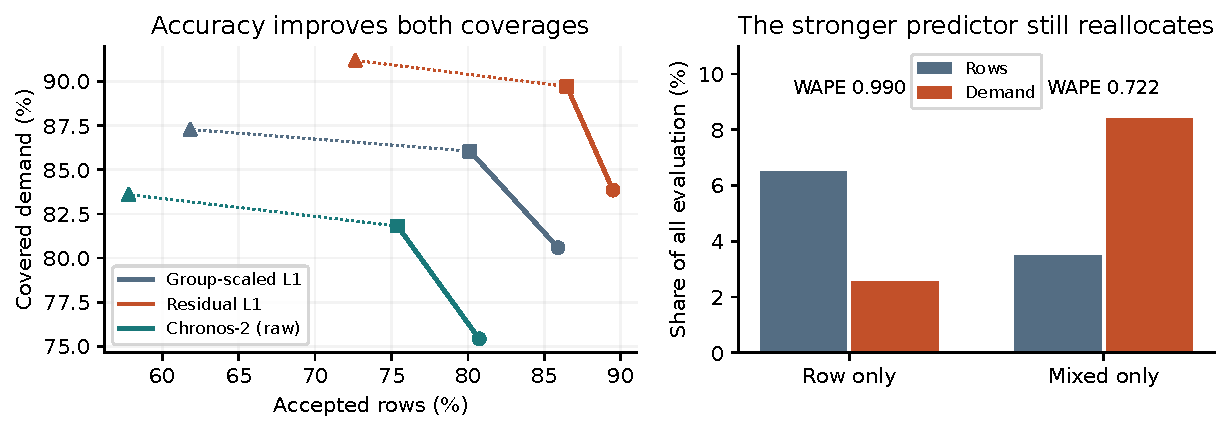
\includegraphics[width=\linewidth]{figures/accuracy_coverage.pdf}
\caption{Matched-date comparison. Left: moving to a stronger predictor raises both coverages, while changing utility within a predictor trades them off. Circles, squares, and triangles denote $\lambda=1,0.25,0$. Lines connect evaluated settings, not Pareto frontiers. Right: the improved predictor's exclusive acceptance sets retain the budget mechanism.}
\label{fig:accuracy}
\end{figure}
The improved mixed policy also exceeds the base row policy in both coverages (86.48/89.72 versus 85.90/80.59 percent). Nevertheless, its row-only set carries just 2.55\% of demand while spending 59.84\% of common slack (Appendix~\ref{app:accuracy}). The smaller case sacrifice (3.02 versus 5.77 points) coexists with the same mechanism. Neither pooled policy establishes the Hobbies or Household cap.


\subsection{What the additional forecasting controls establish}
The preceding forecasting study includes fixed risk-bin recalibration, forecast-value bins, top-risk-only uplift, minimum-support fallback, separately tuned residual learning with and without $q$, and frozen-backbone recalibration. Its role here is to supply stronger predictors and explicit limits on interpretation, not to claim a universally superior risk coordinate.

\begin{table}[htbp]\centering\small
\caption{Retained forecasting controls. All later learned-model comparisons are retrospective. FreshRetailNet non-stockout rows condition on realized availability; all-row metrics target recorded sales, not latent demand. M5 is the first-seed later development block.}
\label{tab:forecast-controls}
\begin{tabular}{lrrr}\toprule
Forecast & M5 & FRN non-stockout & FRN all sales\\\midrule
Group scale & 0.67139 & 0.32928 & 0.36162\\
Forecast-value bins & 0.67045 & 0.32753 & 0.36154\\
Risk bins & 0.66851 & 0.32741 & 0.36033\\
Top-risk-only uplift & 0.66843 & 0.32504 & 0.35938\\
Residual L1 with $q$ & 0.65956 & 0.29201 & 0.33401\\
Residual L1 without $q$ & 0.66532 & 0.29289 & 0.33463\\\bottomrule
\end{tabular}\end{table}

On M5, bin-based recalibration adds only a modest gain over the parent and does not beat the residual learner. On FreshRetailNet, a 2,000-series cohort was fixed from training data before the original one-time seven-day evaluation. Its original risk-bin versus parent comparison has uncertainty sensitive to clustering. Later forecast-bin, uplift, and learned controls reuse this cohort; they are not additional prospective tests. The original non-stockout population contains 8,020 rows, versus 14,000 recorded-sales rows overall. Training/selection for the residual learner uses the chronological tail of the training partition (earlier two blocks for fitting; later three for selection), then refits on all five. The same six-setting grid selects depth 4 and 300 trees. The base, risk head, and categorical encoder remain fixed from earlier training.

FreshRetailNet risk-bin minus residual WAPE is 0.03541 on non-stockout rows. Paired 95\% intervals are [0.02813,0.04273] by series, [0.02824,0.04368] by store, [0.01535,0.05326] by product, and [0.02135,0.04983] by date; only seven dates are available. The no-$q$ follow-up is adaptive and separately tuned. Its WAPE difference from the full residual learner is 0.00088, with product-cluster interval [$-0.00016$,0.00197]. Most forecasting improvement therefore cannot be attributed to the risk feature. The corrected predictor's RMSE decreases from 0.74595 to 0.62157 and signed bias from $-14.04\%$ to $-1.92\%$ on that population. It still worsens 777 of 2,000 series. None of these observations identifies demand on stockout rows or measures inventory cost.

Frozen Chronos recalibration also improves within-backbone WAPE, but its calibration period differs from that of the main tabular predictor and its bin-control advantage changes under asymmetric pinball losses. These historical comparisons are preserved in the forecasting evidence archive. They are not pooled with the original external test or counted as independent natural-demand confirmation. Numerical dependency repairs and column-label audits are recorded there; the selected forecasts used in the present experiment reproduce the corrected reference values exactly.

\section{Additional cap and classification audits}\label{app:new-audits}
\subsection{Why full-coverage failure is not sufficient}\label{app:necessity}
If full-coverage risk is at most $r$, accept-all is feasible and maximizes both coverages. The converse fails even with positive exposure: take two equally probable contexts with $w=1$, $\ell=(0,1)$, and $r=1/4$. Full-coverage risk is $1/2>r$, but feasibility is $3a_2\leq a_1$. The common unique optimum is $(1,1/3)$, with both coverages $2/3$ and risk $1/4$. Any row floor at most $2/3$ leaves this example feasible. Unlike $\ell\equiv0$, this counterexample satisfies the premise of full-coverage cap failure.

\subsection{Development cap/floor sweep and conditional-error baseline}
We reuse the three predictors and their frozen demand and squared-loss error heads from Section~\ref{sec:accuracy}, without fitting or accessing either holdout. The declared grid is $r\in\{.60,.62,.64012983268,.66,.68,.70\}$ and $c_0\in\{0,.35,.60,.80\}$. For each cap we compare conditional error $\hat e$, row excess, mixed utility ($\lambda=.25$), and exposure ratio ($\lambda=0$). The conditional-error comparator instantiates the regression-based uncertainty construction of \citet{franc2023reject}; its threshold is recalibrated to our ratio-risk constraint. This is neither a reproduction of their SELE training objective nor a claim to their original risk guarantees.

For every ranking, we search its distinct finite calibration scores, accepting whole ties, and choose the largest threshold satisfying both chronological calibration blocks. The same rule is applied to all methods. An infeasible family accepts nothing, with undefined risk rather than risk zero. The saved grid contains 288 configurations. At the original cap and floor, all nine previously reported objective-specific thresholds and coverage/risk triples reproduce to $10^{-12}$.

Table~\ref{tab:new-cap} shows the mixed-minus-row contrast. For the base and improved predictors it persists through $.66$, and for Chronos through $.68$. At loose caps both coverages approach one. Tiny remaining differences reflect transfer of finite observed-score thresholds, rather than an explicit accept-all candidate; they are not population reversals. Raising the floor never changes a surviving threshold: 31 grid records become infeasible relative to floor zero. This is the nested-family prediction, and clarifies that a row floor filters feasibility rather than providing an alternative optimum within a fixed ranking. All results remain retrospective and conditional on these fits.

\begin{table}[t]\centering\small
\caption{Development sensitivity at row floor $.35$. Entries are mixed-minus-row case/exposure coverage differences in percentage points. Error-only reports whether the conditional-error family is feasible on calibration A/B.}\label{tab:new-cap}
\begin{tabular}{lrrrr}\toprule
Predictor & Cap & $\Delta c$ & $\Delta d$ & Error-only feasible\\\midrule
Base & 0.600 & -8.64 & +9.22 & no\\
Base & 0.620 & -7.55 & +7.30 & no\\
Base & 0.640 & -5.77 & +5.47 & no\\
Base & 0.660 & -4.85 & +3.01 & no\\
Base & 0.680 & -0.73 & +0.19 & yes\\
Base & 0.700 & +0.00 & +0.05 & yes\\
Improved & 0.600 & -6.46 & +10.27 & no\\
Improved & 0.620 & -4.68 & +8.31 & no\\
Improved & 0.640 & -3.02 & +5.87 & no\\
Improved & 0.660 & -1.69 & +2.01 & no\\
Improved & 0.680 & +0.00 & +0.08 & yes\\
Improved & 0.700 & +0.00 & +0.09 & yes\\
Chronos-2 & 0.600 & -8.25 & +9.76 & no\\
Chronos-2 & 0.620 & -6.49 & +7.89 & no\\
Chronos-2 & 0.640 & -5.35 & +6.39 & no\\
Chronos-2 & 0.660 & -5.10 & +5.10 & no\\
Chronos-2 & 0.680 & -3.80 & +1.35 & no\\
Chronos-2 & 0.700 & +0.00 & +0.05 & yes\\
\bottomrule\end{tabular}\end{table}

\subsection{Yeast: a prespecified real-data negative check}
We use the official Mulan Yeast train/test files (1,500/917 examples, 103 features, 14 labels; \url{https://github.com/tsoumakas/mulan/tree/master/data/multi-label/yeast}). Before evaluating test labels, we record the protocol, then fit independent standardized logistic classifiers on 1,125 training examples and calibrate on the remaining 375 (seed 20260909). Each classifier has $C=1$ and a fixed $.5$ probability threshold. Whole-example acceptance retains or removes every predicted label together. The observed weight is the number of predicted positives, and loss is the number of false positives; thus risk is one minus micro-precision, not false negatives or true-positive coverage. Estimated loss sums $1-\hat p_j$ over predicted-positive labels. Zero-weight examples also have zero loss and are accepted freely.

The primary cap is $.85$ times calibration full-coverage risk; $.75$, $.95$, and $1.05$ are secondary declared factors. The row floor is $.35$. Conditional error, row excess, and exposure-ratio thresholds use the same largest-feasible whole-tie rule. Model files and thresholds are frozen before the single test-label read. The frozen classifier's test exposure ranges from zero to seven (nine zero-weight examples), and full risk is $.33956$.

At the primary cap $.27559$, both objective-specific policies accept 574/917 examples. Exposure coverage changes from $62.850\%$ to $62.941\%$: $+0.090$ points with paired example-bootstrap 95\% interval $[-0.181,0.452]$. The case difference is zero, with interval $[-0.327,0.327]$ points. Both test point risks exceed the cap. This does not establish strict objective reversal on Yeast, despite varying exposure. It is consistent with the distinction between an existence theorem and outcomes of estimated scores. We retain the negative result rather than replacing the primary cap after seeing test outcomes. Table~\ref{tab:new-yeast} reports every declared policy; secondary contrasts and all masks are in the supplement. The 2,000-resample intervals condition on the fit and are marginal, not simultaneous over the cap grid.

\begin{table}[t]\centering\small
\caption{All prespecified Yeast test results. Cap factors multiply the calibration full risk. Coverage is in percent; risk is false positives per predicted positive.}\label{tab:new-yeast}
\begin{tabular}{rlrrr}\toprule
Factor & Ranking & Cases & Exposure & Risk\\\midrule
0.75 & Conditional error & 42.86 & 34.05 & 0.2354\\
0.75 & Row excess & 37.95 & 36.49 & 0.2263\\
0.75 & Exposure ratio & 38.60 & 36.46 & 0.2223\\
0.85 & Conditional error & 67.50 & 59.20 & 0.2840\\
0.85 & Row excess & 62.60 & 62.85 & 0.2910\\
0.85 & Exposure ratio & 62.60 & 62.94 & 0.2896\\
0.95 & Conditional error & 92.15 & 88.76 & 0.3269\\
0.95 & Row excess & 86.48 & 86.11 & 0.3202\\
0.95 & Exposure ratio & 83.97 & 85.36 & 0.3187\\
1.05 & Conditional error & 100.00 & 100.00 & 0.3396\\
1.05 & Row excess & 99.67 & 99.61 & 0.3382\\
1.05 & Exposure ratio & 99.89 & 99.97 & 0.3394\\
\bottomrule\end{tabular}\end{table}

\section{Non-retail checks and additional diagnostics}\label{app:nonretail}
\subsection{Design fixed before the new evaluations}
After the Yeast result, we specify two additional datasets, a single seed (20260910), models, all selectors, primary reporting cap factor $.85$, and secondary factors $\{.75,.95,1.05\}$. Each reporting cap multiplies full calibration risk. Thresholds must satisfy $.95$ times that cap on calibration, supplying a fixed margin rather than a guarantee, and row coverage at least $.35$. Methods rank by predicted error, signed row excess, mixed utility ($\lambda=.25$), exposure ratio, or descending predicted weight. Every distinct calibration score is considered with whole ties; accept-all is also included when calibration permits it. Infeasible methods return an empty set and undefined risk. Results at loose reporting caps may still reject cases because calibration uses a margin.

UCI Bike Sharing (\url{https://archive.ics.uci.edu/dataset/275/bike+sharing+dataset}) supplies recorded hourly rentals, not latent unconstrained demand. We randomize days into 40/20/20/20 percent predictor-fit, error-head-fit, calibration, and test groups. Calendar and contemporaneous weather variables are features; counts and their registered/casual components are excluded. Fixed LightGBM models use 200 trees, 31 leaves, learning rate $.05$, and minimum leaf sample count 30. The point predictor uses median loss; a Poisson head estimates mean exposure. Squared-loss regression estimates absolute errors on a disjoint head-fit partition. No censoring is introduced. The 3,477-hour test has 147 days. This split tests conditional prediction on new day groups, not chronological extrapolation with forecast weather.

Delicious uses the LIBSVM redistribution of Mulan (\url{https://www.csie.ntu.edu.tw/~cjlin/libsvmtools/datasets/multilabel.html}), with 500 supplied features and 983 labels. A seeded 60/20/20 row split separates fitting, calibration, and testing. Independent logistic classifiers use $C=1$, liblinear, and fixed probability threshold $.5$ (primary) or $.2$ (secondary). Weight is the predicted-positive count and loss is false-positive count. Test labels are parsed only after the model and all thresholds are frozen. At the primary cap, neither objective-specific family can meet the calibration constraint and row floor. This remains a negative result; empty-set intervals are not evidence of equivalence between useful policies.

For each dataset we retain all declared results and perform 4,000 paired resamples of test units: days for Bike Sharing and examples for Delicious. Marginal 95\% intervals and 98.75\% percentile intervals are supplied. The latter apply a Bonferroni adjustment over two coverage differences in each of the two primary dataset comparisons, conditional on fitted models. They are approximate bootstrap statements, not distribution-free risk guarantees. No model or cap was changed after test evaluation. The subsequent menu audit in Table~\ref{tab:policy-choice} adjusts eight coverage endpoints at 99.375\%, using a separate declared bootstrap seed; the two interval families answer different reporting scopes, not independent replications.

\subsection{Mobility reversal and its budget}
At the primary cap, demand-minus-row coverage is $-13.34$ case points and $+5.01$ exposure points. The adjusted intervals are $[-15.86,-10.77]$ and $[2.27,8.16]$ points. Both test point risks are below $.13281$. The common set has 2,460 hours and supplies 5,219.29 loss units of slack. Row-only acceptance adds 596 hours and 15,531 rentals, costing 3,568.63; demand-only acceptance adds 132 hours and 49,847 rentals, costing 2,399.22. The union has risk $.13398$ and excess $+748.56$: these two observed additions cannot both fit the reporting cap. This decomposition is descriptive and was not a prespecified endpoint. The later risk audit finds that row, ratio, and union intervals all cross the cap (Appendix~\ref{app:policy-choice}); the budget comparison is therefore a sample-level result, not a joint population feasibility claim. In contrast, the original retail external sets have a feasible union; that experiment verifies a selected policy contrast rather than binding competition.

\begin{table}[t]\centering\small
\caption{Mobility primary test, cap $.13281$. Error-only is infeasible at calibration. Coverage is percent.}\label{tab:mobility}
\begin{tabular}{lrrr}\toprule
Ranking & Cases & Exposure & Risk\\\midrule
Conditional error & 0.00 & 0.00 & --\\
Row excess & 87.89 & 85.54 & 0.12999\\
Mixed & 86.54 & 89.66 & 0.12962\\
Exposure ratio & 74.55 & 90.56 & 0.12826\\
Descending mean & 37.79 & 73.66 & 0.12396\\
\bottomrule\end{tabular}\end{table}

\subsection{Descending-demand baseline on M5}
For the original cap and row floor, we use exactly the same two-block threshold calibration as the earlier sweep, substituting $-\hat\mu$ for the score. Table~\ref{tab:descending} shows that this simple ranking covers more demand than the fitted pure-ratio rule in all three cases, but accepts fewer rows. This refutes a universal empirical-superiority interpretation of estimated ratio ranking; it does not contradict the exact-conditional-information theorem.
\begin{table}[t]\centering\small
\caption{Descending predicted demand at the original M5 cap; development evaluation only.}\label{tab:descending}
\begin{tabular}{lrrr}\toprule Predictor & Cases (\%) & Demand (\%) & WAPE\\\midrule
Base & 45.24 & 88.24 & 0.62696\\
Improved & 54.32 & 92.15 & 0.63058\\
Chronos-2 & 41.14 & 86.06 & 0.62997\\
\bottomrule\end{tabular}\end{table}

\subsection{Rank agreement as a diagnostic, not a certificate}
On positive estimated exposure, Kendall's $\tau$ between row-excess and ratio rankings is $.872$ for Yeast, $.300/.298/.347$ for the three M5 predictors, $.635$ for Bike Sharing, and $.760$ for Delicious's primary classifier. M5 uses a seeded 100,000-row sample; the smaller datasets use all test examples. The high Yeast agreement is consistent with similar acceptance sets, while lower agreement indicates scope for different allocations. Agreement alone does not determine thresholds, feasibility, exposure masses, or their generalization. In particular, Delicious is infeasible despite nonidentical rankings. These associations are descriptive, not an identified causal explanation or a necessary-and-sufficient diagnostic. Zero-exposure cases are excluded from the correlation and are not silently included in a positive-lower-bound envelope.
\begin{table}[t]\centering\scriptsize
\caption{Declared secondary non-retail results: row and exposure rankings. A dash denotes calibration infeasibility, not zero risk. All five ranking families are in the accompanying JSON records.}
\begin{tabular}{llrrrrrr}\toprule
Data/threshold & Factor & Row $c$ & Row $d$ & Row risk & Ratio $c$ & Ratio $d$ & Ratio risk\\\midrule
Bike & 0.75 & 61.92 & 58.61 & 0.1124 & 57.95 & 78.85 & 0.1203\\
Bike & 0.85 & 87.89 & 85.54 & 0.1300 & 74.55 & 90.56 & 0.1283\\
Bike & 0.95 & 95.48 & 94.71 & 0.1398 & 91.54 & 97.64 & 0.1406\\
Bike & 1.05 & 100.00 & 100.00 & 0.1515 & 99.63 & 99.97 & 0.1513\\
Delicious 0.2 & 0.75 & 0.00 & 0.00 & -- & 0.00 & 0.00 & --\\
Delicious 0.2 & 0.85 & 0.00 & 0.00 & -- & 0.00 & 0.00 & --\\
Delicious 0.2 & 0.95 & 0.00 & 0.00 & -- & 0.00 & 0.00 & --\\
Delicious 0.2 & 1.05 & 98.70 & 98.80 & 0.6380 & 97.76 & 98.65 & 0.6380\\
Delicious 0.5 & 0.75 & 0.00 & 0.00 & -- & 0.00 & 0.00 & --\\
Delicious 0.5 & 0.85 & 0.00 & 0.00 & -- & 0.00 & 0.00 & --\\
Delicious 0.5 & 0.95 & 0.00 & 0.00 & -- & 0.00 & 0.00 & --\\
Delicious 0.5 & 1.05 & 97.86 & 99.05 & 0.4242 & 94.19 & 98.48 & 0.4239\\
\bottomrule\end{tabular}\end{table}

\subsection{Original point-forecast adapter specifications}\label{app:original-adapter}
The reference forecaster fits histogram gradient boosting with Poisson loss to observed sales. Its expectation--maximization (EM) correction repeatedly imputes censored responses using clipped Poisson means conditional on exceeding capacity, then refits; a separate classifier predicts censoring probability. New LightGBM controls share origin-valid features, 1.2 million sampled rows, 300 trees, 63 leaves, learning rate 0.05, and three seeds. Objectives are Poisson or L1 on observed sales, with an uncensored-row-only L1 ablation. For L1 forecast $b$, the adapter reuses the earlier EM prediction $e_{\rm EM}$ and predicted censor probability $\hat p_C$:
\begin{equation}
 f_{\alpha,\gamma}=b+\alpha\hat p_C^\gamma\max(e_{\rm EM}-b,0).
 \label{eq:adapter}
\end{equation}
Only point selection chooses $\alpha,\gamma$. Controls include global/category rescaling and the same ungated correction. The supervised selector comparisons retain the first point seed and $(\alpha,\gamma)=(2,2)$. The sales-and-capacity extension uses the plain observed-sales L1 forecaster without this adapter.


\section{Choosing a rule by its intended coverage utility}
\label{app:policy-choice}

\subsection{Scope and fixed analysis}
This additional analysis reuses published calibration and evaluation arrays. Its analysis specification was recorded before the new comparisons were computed, but the research program had already examined these outcomes. It is a retrospective audit, not a fresh holdout experiment. No predictor or risk head is fitted; no external retail partition is reopened. The original frozen objects, protocols, and negative results are unchanged.

The fixed menu has five rankings in tie order: conditional error, row excess, mixed utility ($\lambda=.25$), pure exposure ratio, and descending predicted exposure. The last is a simple baseline. The error-regression score instantiates the regression-based uncertainty construction discussed by \citet{franc2023reject}; it is not a reproduction of SELE, SelectiveNet, or their original objectives. The menu audit uses exactly the same features and fitted heads for both utility choices.

For each ranking we search every distinct calibration score, retain entire ties, and explicitly check accept-all. Empirical risk need not be monotone in a ranked prefix; the chosen threshold is the largest prefix satisfying all prescribed window constraints. Case and exposure utilities both increase along a nested family, so they cannot choose different thresholds within that family. They select between the five candidate gates by minimum calibration-window coverage. Exact ties follow the declared order. A menu with no feasible gate returns no selection and an undefined accepted risk rather than risk zero.

The primary M5 cap is $r=.85\times.7530939208$, with a .35 case floor in both A/B windows. Bike retains its original cap of .85 times full calibration risk, .95 design margin, and .35 floor. The full M5 cap grid is $\{.60,.62,.64012983268,.66,.68,.70\}$; Bike uses multipliers $\{.75,.85,.95,1.05\}$. No evaluation-period winner is used to choose a threshold or rule. At accept-all, the method label ``error'' is only the declared tie breaker; it is not evidence of error-ranking superiority.

\begin{table}[t]
\centering\scriptsize
\caption{Declared cap sensitivity of utility-based menu selection. M5 uses absolute caps; Bike lists multipliers of full calibration risk. Changes are evaluation exposure-choice minus case-choice, in percentage points. ``All'' denotes an identical accept-all policy, regardless of its tie-breaking method label. These are descriptive additional comparisons.}
\label{tab:choice-caps}
\begin{tabular}{lllr r}
\toprule
Setting & Cap / multiplier & Case / exposure rule & $\Delta c$ & $\Delta d$ \\
\midrule
M5: L1 & 0.600 & Excess / Ratio & -28.94 & 11.50 \\
M5: L1 & 0.620 & Excess / Ratio & -27.73 & 9.12 \\
M5: L1 & 0.640 & Excess / Exposure descending & -40.66 & 7.64 \\
M5: L1 & 0.660 & Excess / Exposure descending & -37.70 & 4.16 \\
M5: L1 & 0.680 & Error / Exposure descending & -15.72 & 0.83 \\
M5: L1 & 0.700 & All / All & 0.00 & 0.00 \\
M5: residual & 0.600 & Excess / Ratio & -25.44 & 13.05 \\
M5: residual & 0.620 & Excess / Exposure descending & -36.86 & 12.08 \\
M5: residual & 0.640 & Excess / Exposure descending & -35.18 & 8.31 \\
M5: residual & 0.660 & Excess / Exposure descending & -24.33 & 2.96 \\
M5: residual & 0.680 & All / All & 0.00 & 0.00 \\
M5: residual & 0.700 & All / All & 0.00 & 0.00 \\
M5: Chronos-2 & 0.600 & Excess / Ratio & -26.14 & 12.52 \\
M5: Chronos-2 & 0.620 & Excess / Ratio & -25.59 & 10.22 \\
M5: Chronos-2 & 0.640 & Excess / Exposure descending & -39.61 & 10.63 \\
M5: Chronos-2 & 0.660 & Excess / Exposure descending & -38.20 & 7.90 \\
M5: Chronos-2 & 0.680 & Excess / Exposure descending & -29.84 & 2.93 \\
M5: Chronos-2 & 0.700 & All / All & 0.00 & 0.00 \\
Bike Sharing & 0.750 & Mixed / Ratio & -8.51 & 4.16 \\
Bike Sharing & 0.850 & Excess / Ratio & -13.34 & 5.01 \\
Bike Sharing & 0.950 & Excess / Ratio & -3.94 & 2.93 \\
Bike Sharing & 1.050 & Error / Error & 0.00 & 0.00 \\
\bottomrule
\end{tabular}
\end{table}


\subsection{Coverage differences and resampling}
For the three M5 predictors and Bike, the two primary differences are exposure-choice minus case-choice in case and exposure coverage. We use 4,000 paired bootstrap draws (seed 20260911), resampling items for M5 and days for Bike. The eight primary endpoints use 99.375\% percentile intervals, corresponding to a Bonferroni adjustment. This is an approximate, fit-conditional analysis: it omits selection and training uncertainty and does not remove shared calendar or store dependence. The three M5 predictors share data and do not constitute independent replications.

For L1, residual, and Chronos, adjusted case-difference intervals are respectively $[-43.71,-37.72]$, $[-38.08,-32.42]$, and $[-42.72,-36.67]$ points. Bike's interval is $[-16.23,-10.61]$. Table~\ref{tab:policy-choice} reports the exposure intervals. All eight exclude zero. The primary M5 selected point risks lie below the cap, but their pointwise 95\% intervals cross it. Consequently those menu comparisons do not by themselves establish risk feasibility in the population.

The selected exposure rule also illustrates estimation limits. Descending predicted exposure beats the fitted pure-ratio rule in all three primary M5 comparisons, but is not chosen on Bike. Tightening the cap can change the M5 choice to the ratio. This is a result about selecting within the declared menu, not evidence that one fitted ranking is universally optimal or that every ranking inversion is caused by small denominators.

\subsection{A separate-window approximate risk screen}
\label{sec:risk-screen}
We repeat threshold design on A alone with the fixed design cap $.95r$ and .35 case floor. For each of the 15 possible predictor--ranking pairs, the resulting threshold is then held fixed on B. Define item-level signed excess
\[
 G_{ij}=\sum_{t\in i}a_j(X_t)(L_t-rW_t).
\]
The screening value is the one-sided bootstrap upper percentile of mean $G_{ij}$ at level $1-.05/15$, using the same 4,000 item resamples for all candidates. A candidate passes if this value is nonpositive and its accepted exposure is positive. Utility selection among passing candidates uses A only. B is neither used to move a threshold nor to rank utility. The screen's sign corresponds to a ratio cap because the denominator is positive; this does not turn the bootstrap into a finite-sample distribution-free test.

Ten candidates have a feasible A threshold, and all ten pass the adjusted B screen. The other five fail at threshold design: all three error-only rankings and descending exposure for L1 and Chronos. Thus this particular B screen does not reject an A-feasible candidate; the observed margin is obtained by the stricter A design, with B providing a separate check. Upper bounds on mean B signed excess for the ten candidates range from $-5.94$ to $-1.45$ per item. The software retains the no-choice branch if all candidates fail, rather than relaxing the cap or floor.

\begin{table}[t]
\centering\small
\caption{Two-window risk screen on M5. Thresholds use A with design cap $0.95r$; a separate B item-bootstrap check tests signed excess at reporting cap $r=0.64013$, with Bonferroni adjustment over all 15 candidates. All six selected policies pass that approximate B screen. Later risk intervals below are pointwise 95\%, conditional on fits and selected policies.}
\label{tab:policy-screen}
\begin{tabular}{lllrrl}
\toprule
Predictor & Utility & Rule & $c$ (\%) & $d$ (\%) & Later risk [95\% interval] \\
\midrule
M5: L1 & Cases & Excess & 72.50 & 70.58 & 0.6015 [0.5816, 0.6223] \\
M5: L1 & Exposure & Ratio & 44.16 & 79.11 & 0.5974 [0.5800, 0.6154] \\
M5: residual & Cases & Excess & 75.36 & 72.92 & 0.6009 [0.5807, 0.6220] \\
M5: residual & Exposure & Exposure descending & 38.80 & 84.68 & 0.5984 [0.5807, 0.6167] \\
M5: Chronos-2 & Cases & Excess & 67.74 & 65.75 & 0.6039 [0.5831, 0.6257] \\
M5: Chronos-2 & Exposure & Ratio & 41.63 & 74.79 & 0.5959 [0.5776, 0.6144] \\
\bottomrule
\end{tabular}
\end{table}


The later-period exposure-choice gains for L1, residual, and Chronos are 8.52, 11.76, and 9.04 points; corresponding descriptive 95\% intervals are $[7.15,9.92]$, $[9.59,14.12]$, and $[7.92,10.12]$. Case differences are $-28.34$, $-36.55$, and $-26.11$ points, with intervals $[-30.06,-26.62]$, $[-38.82,-34.28]$, and $[-27.78,-24.45]$. For the residual predictor, case-selected coverage falls from 89.50\% in the original menu to 75.36\% after the stricter design. These are secondary, retrospective contrasts. Table~\ref{tab:policy-screen}'s six risk intervals are pointwise rather than a joint test family. The stricter design sacrifices coverage and establishes no groupwise or shifted-deployment guarantee. The historical external operating checks are unchanged.

\subsection{Bike risk uncertainty and budget interpretation}
An additional descriptive replay uses the original Bike bootstrap seed 20260910 and all 147 test days. At the reporting cap $r=.1328061$, row and ratio risks are .129987 and .128257; their union risk is .133984. Pointwise 95\% day-bootstrap intervals are $[.120321,.140896]$, $[.118432,.139444]$, and $[.123871,.145496]$. Bonferroni-adjusted intervals over these three quantities are $[.118419,.143363]$, $[.116489,.142088]$, and $[.121677,.147828]$. All cross the cap. The same replay exactly reproduces the original 98.75\% coverage-difference intervals.

The sample-level budget identity is exact, but joint population claims require more evidence: that each policy meets the cap, their union exceeds it, and both coverage contrasts have the prescribed signs. The present risk intervals establish neither feasibility nor infeasibility for those population risks. Even a confirmed infeasible union would not establish that the original policies are Pareto-optimal: a third gate could dominate them.

\subsection{Executable audit and complete outputs}
\texttt{code/policy\_audit.py} exposes threshold design, utility selection, and sufficient-statistic functions; none accepts evaluation labels during design. \texttt{code/run\_policy\_choice.py} writes frozen choices before computing evaluation metrics. The full output retains all 22 menu settings, all 15 screen candidates, input hashes, and cluster sufficient statistics. \texttt{code/verify\_policy\_choice.py} independently checks the selected utility, old frozen-threshold compatibility, accounting identities, and bootstrap replay. \texttt{code/replay\_bike\_risk\_audit.py} reconstructs the three original risk intervals. Reproduction commands write to separate output directories.

\subsection{The coverage definition changes the selected rule}
\label{sec:policy-choice}
\begin{table}[t]
\centering\small
\caption{Coverage changes the selected rule. Thresholds and the case/exposure choices use calibration outcomes only. Differences are exposure-choice minus case-choice on evaluation data (percentage points). Intervals are paired cluster-bootstrap 99.375\% intervals, adjusted across the eight primary coverage contrasts; all eight exclude zero. These additional menu comparisons are retrospective.}
\label{tab:policy-choice}
\begin{tabular}{llrr}
\toprule
Setting & Selected by cases / exposure & $\Delta c$ & $\Delta d$ [adjusted interval] \\
\midrule
M5: L1 & Excess / Exposure descending & -40.66 & 7.64 [4.24, 11.97] \\
M5: residual & Excess / Exposure descending & -35.18 & 8.31 [5.47, 11.69] \\
M5: Chronos-2 & Excess / Exposure descending & -39.61 & 10.63 [7.37, 14.49] \\
Bike Sharing & Excess / Ratio & -13.34 & 5.01 [1.93, 8.56] \\
\bottomrule
\end{tabular}
\end{table}

Case coverage chooses the excess ranking for all four primary menus. Exposure coverage chooses descending predicted demand for all three retail predictors and the fitted ratio for Bike. Thus the practical implication is not to prescribe one score everywhere: the utility determines which candidate to select, and the empirical winner depends on the task.

These calibration choices retain their coverage contrast on evaluation data (Table~\ref{tab:policy-choice}). For the residual predictor, changing the selected rule raises covered demand from 83.85\% to 92.15\% while reducing accepted cases from 89.50\% to 54.32\%. All eight adjusted coverage intervals exclude zero. The three retail comparisons share items, and this additional analysis is retrospective. It measures the consequence of selecting among these five rules, not a general benchmark ranking of uncertainty estimators.

\begin{figure}[t]
\centering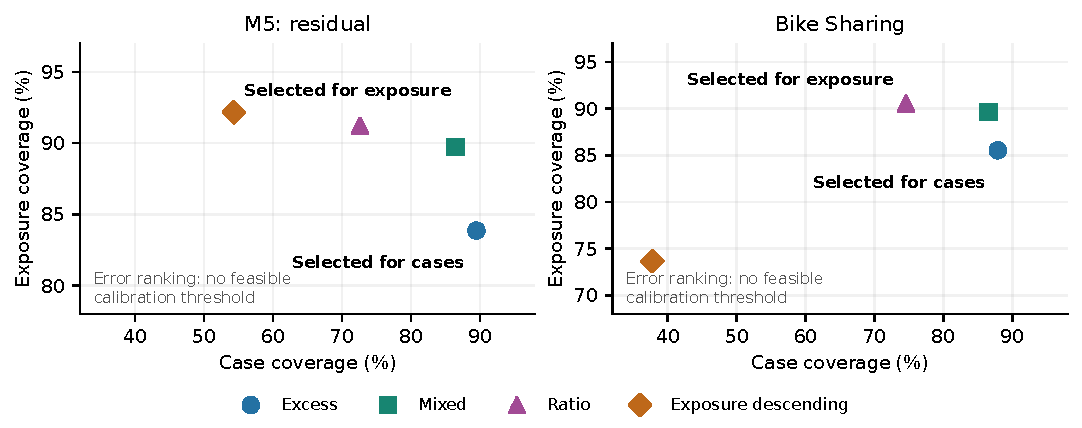
\includegraphics[width=\linewidth]{figures/policy_choice.pdf}
\caption{One predictor and one calibration-feasible candidate menu per panel. Labels identify rules selected by calibration utility; coordinates are evaluation coverages. The exposure choice is the simple descending-exposure baseline on M5 and the ratio on Bike. No line is drawn as a Pareto frontier. Point-risk feasibility does not imply a certified risk bound.}
\label{fig:policy-choice}
\end{figure}

The cap sweep also changes the exposure-selected family: the fitted ratio is selected at stricter retail caps, whereas descending predicted exposure is selected at the original cap. At a sufficiently loose cap both choices accept all and the contrast vanishes. The conditional-error ranking has no feasible threshold at the primary caps under the stated floor. Every declared cap is retained in Appendix Table~\ref{tab:choice-caps}. At .68 only the residual predictor has zero contrast; L1 and Chronos retain it. Cap dependence is part of the result, not evidence for a universally preferred cap or score.


\section{Paired histories and untuned head sensitivity}\label{app:matched}
The added experiment refits two median-loss LightGBM predictors, each with 300 trees, 31 leaves, learning rate .05, minimum leaf size 50, and seed 20260910. Both use exactly the same 600,000 sampled rows on days 1314--1554. One arm uses artificially censored sales for histories and fit targets; the other uses complete recorded sales. This removes artificial censoring, not possible natural stockouts in the original records. The two arms use the same 28 common feature definitions and six item-aggregate history features. Capacity, fill-ratio, censor-rate, and hit-rate features are excluded from both arms. Price features use the origin week. All history aggregates are rebuilt for each arm.

A disjoint 600,000-row sample on days 1555--1610 fits each arm's conditional absolute-error and exposure heads. Both use squared loss with either 220 or 660 trees; all other tree parameters remain fixed. The tree counts are not selected by validation or early stopping, so this comparison does not test an improvement in conditional-moment estimation. Their four combinations share the point predictor. Targets for these audit heads are complete sales and realized absolute error. Realized outcomes are noisy targets for conditional moments; substituting them directly into a test selector would not be a conditional-information oracle.

Calibration A/B and evaluation dates match the earlier development audit. All five rankings receive their largest complete-tie threshold meeting both calibration caps and the .35 case floor. The primary cap is .95 times the larger full-coverage A/B risk for that arm. The absolute grid is $\{.60,.62,.64012983268,.66,.68,.70\}$; relative factors are $\{.85,.90,.95,1,1.05\}$. Only the primary relative cap receives the full head factorial; all grid points use the 220-tree heads. Utility choices, model hashes, and thresholds are saved before each arm's new evaluation. The protocol fixes both arms before fitting. All dates were previously evaluated, so this is retrospective evidence, not a new external trial. Intervals use 2,000 paired item resamples, conditional on the fits, and are descriptive 95\% intervals without a simultaneous-risk claim.

\begin{table}[t]\centering\scriptsize
\caption{Untuned tree-count sensitivity at each arm's primary cap. Error/exposure head tree counts vary factorially, with the point predictor fixed; tree counts were not selected by validation or early stopping. Larger heads are not uniformly more accurate, so these comparisons do not test whether improved moment estimates resolve the choice. MSE is evaluated against realized error or sales, not observed conditional moments.}\label{tab:matched-heads}
\begin{tabular}{llrrlrr}\toprule
Arm & Trees $e/w$ & Error MSE & Exposure MSE & Case / exposure rule & $\Delta c$ & $\Delta d$\\\midrule
Artificially censored & 220 / 220 & 4.475 & 5.893 & Excess / Exposure descending & -39.95 & +7.05 \\
Artificially censored & 660 / 220 & 4.510 & 5.893 & Excess / Exposure descending & -40.66 & +8.29 \\
Artificially censored & 220 / 660 & 4.475 & 5.883 & Excess / Exposure descending & -37.94 & +8.08 \\
Artificially censored & 660 / 660 & 4.510 & 5.883 & Excess / Exposure descending & -40.04 & +8.14 \\
Complete recorded sales & 220 / 220 & 3.064 & 4.761 & Excess / Ratio & -15.81 & +9.72 \\
Complete recorded sales & 660 / 220 & 3.119 & 4.761 & Excess / Exposure descending & -34.52 & +11.45 \\
Complete recorded sales & 220 / 660 & 3.064 & 4.805 & Excess / Exposure descending & -34.85 & +9.88 \\
Complete recorded sales & 660 / 660 & 3.119 & 4.805 & Excess / Exposure descending & -34.98 & +10.71 \\\bottomrule\end{tabular}\end{table}

\begin{table}[t]\centering\scriptsize
\caption{All declared cap settings for the two refitted arms, using the 220-tree heads. Relative caps use the arm-specific maximum full A/B calibration risk. A missing contrast means no eligible policy, not equivalence.}\label{tab:matched-caps}
\begin{tabular}{llrlrr}\toprule
Arm & Cap specification & Risk cap & Case / exposure rule & $\Delta c$ & $\Delta d$\\\midrule
Artificially censored & absolute 0.600 & 0.6000 & Excess / Mixed & -12.25 & +9.86 \\
Artificially censored & absolute 0.620 & 0.6200 & Excess / Ratio & -28.79 & +10.45 \\
Artificially censored & absolute 0.640 & 0.6401 & Excess / Exposure descending & -40.23 & +10.83 \\
Artificially censored & absolute 0.660 & 0.6600 & Excess / Exposure descending & -40.37 & +7.70 \\
Artificially censored & absolute 0.680 & 0.6800 & Excess / Ratio & -18.64 & +4.15 \\
Artificially censored & absolute 0.700 & 0.7000 & Error / Error & +0.00 & +0.00 \\
Artificially censored & relative 0.850 & 0.5947 & Excess / Mixed & -12.19 & +10.26 \\
Artificially censored & relative 0.900 & 0.6297 & Excess / Ratio & -28.29 & +9.71 \\
Artificially censored & relative 0.950 & 0.6647 & Excess / Exposure descending & -39.95 & +7.05 \\
Artificially censored & relative 1.000 & 0.6997 & Error / Error & +0.00 & +0.00 \\
Artificially censored & relative 1.050 & 0.7347 & Error / Error & +0.00 & +0.00 \\
Complete recorded sales & absolute 0.600 & 0.6000 & Excess / Ratio & -22.87 & +14.92 \\
Complete recorded sales & absolute 0.620 & 0.6200 & Excess / Exposure descending & -36.26 & +12.36 \\
Complete recorded sales & absolute 0.640 & 0.6401 & Excess / Ratio & -13.21 & +8.75 \\
Complete recorded sales & absolute 0.660 & 0.6600 & Excess / Ratio & -4.06 & +4.41 \\
Complete recorded sales & absolute 0.680 & 0.6800 & Error / Error & +0.00 & +0.00 \\
Complete recorded sales & absolute 0.700 & 0.7000 & Error / Error & +0.00 & +0.00 \\
Complete recorded sales & relative 0.850 & 0.5661 & Excess / Ratio & -25.84 & +18.69 \\
Complete recorded sales & relative 0.900 & 0.5994 & Excess / Ratio & -23.03 & +14.98 \\
Complete recorded sales & relative 0.950 & 0.6327 & Excess / Ratio & -15.81 & +9.72 \\
Complete recorded sales & relative 1.000 & 0.6660 & Error / Error & +0.00 & +0.00 \\
Complete recorded sales & relative 1.050 & 0.6993 & Error / Error & +0.00 & +0.00 \\\bottomrule\end{tabular}\end{table}


The source package records ten model fits and zero external openings. The verifier independently reconstructs score masks, accepted masses and coverage differences, checks paired evaluation targets and training chronology, and replays the primary intervals. The post-fit moment audit additionally decomposes estimated-minus-realized excess into $(\hat E-E)-r(\hat M-M)$ on each selected set. This is descriptive accepted-mass accounting, not identification of the true conditional heads.

\paragraph{Accepted-mass diagnostics.}
For the complete-sales primary ratio policy, predicted accepted error exceeds realized error by 5.05\%, while predicted accepted exposure exceeds realized exposure by 3.32\%. The corresponding predicted and realized risks are .6390 and .6284. For descending exposure these biases are 6.52\% and 2.91\%, with risks .6516 and .6296. The aggregate discrepancy contains nonzero error and exposure terms; it cannot be described by its denominator term alone. These post-fit aggregate diagnostics do not identify conditional estimation error.

The complete-sales primary common set has 1,313,818 rows, exposure 2,225,652, and error 1,340,939.17. Case-only and exposure-only sets have exposure 135,897 and 419,613, respectively. Their union has risk .6467 versus cap .6327. Descriptive 95\% item-bootstrap risk intervals are [.6065,.6466] for the case policy, [.6106,.6482] for the exposure policy, and [.6283,.6668] for the union; all cross the cap. No joint population feasibility claim follows from the point-budget decomposition.

\FloatBarrier
\section{Retrospective calibration audits added in revision v7}
\label{app:v7}
These analyses use existing predictions and already-consumed development data. They add no model fits, datasets, or external holdout openings. Their protocols and input/code hashes were recorded before the new computations. They are not prospective confirmation or population risk certification. The paired protocol specified the .95 relative cap and the full $2\times2$ head factorial; 220/220 is a reference configuration, not a separately prespecified primary cell.

\subsection{Experiment correspondence}
\begin{table}[H]\centering\scriptsize\setlength{\tabcolsep}{4pt}
\caption{Predictors, heads, caps and evidential roles. The main paired experiment has two predictors; the archived comparison has three different predictors. Reusing them in audits does not add independent model fits or replications. M5 dates below are dataset day indices.}\label{tab:experiment-map}
\begin{tabular}{p{.16\linewidth}p{.27\linewidth}p{.22\linewidth}p{.26\linewidth}}\toprule
Design & Predictor and head fitting & Calibration rule & Evaluation and role\\\midrule
Paired M5, two arms & Median LightGBM, 300 trees, days 1314--1554. Censored or complete histories/targets. Squared-loss error/exposure heads, 220/660 trees, days 1555--1610. & A 1611--1645; B 1646--1673. Primary $r=.95\max(R_A,R_B)$: .664708 censored; .632683 complete. Floor .35 in both. & Later 1800--1913. Seed 20260910; previously used items and periods. All eight head cells in Table~\ref{tab:matched-history}.\\
Archived M5, three predictors & XGBoost L1 hierarchy (750 trees, days 365--1313); hierarchy plus LightGBM L1 residual (selection 1314--1433, final depth 4/300 trees); frozen Chronos-2 median (context 2048, horizon 7, no task fine-tuning). Error/exposure heads: 220-tree squared-loss LightGBM, days 1555--1610. & Same A/B dates. Common reporting cap .640130; floor .35. Ordinary menu uses both windows. Archived screen designs on A at $.95r$ and checks 15 candidates on B. & Same Later window, supplementary predictor comparison; head seed 20260908. Separate from paired refits and the original external test (Appendix~\ref{app:external}).\\
V7 complete-sales screen & Reuses the complete-sales predictor and all four fitted head pairs. No refitting. & A design cap .601049; B screen at .632683; 20 candidates, tail .05/20. Utility uses A among B passers. & Previously used Later window; new conditional bootstrap summaries, no fresh confirmation.\\
V7 stability audit & Reuses complete-sales heads (four pairs) and the Bike models below. & Original caps fixed. Fixed thresholds: 4,000 draws. Threshold redesign: 200 draws for complete 220/220 and Bike. & Calibration only; no evaluation labels read. Item clusters for M5; day clusters for Bike.\\
Bike, supplementary & Median LightGBM, 200 trees, on 292 randomized days; Poisson exposure head on the same fit group; squared-loss error head on 146 other days. Seed 20260910. & 146 days (3,486 hours). Reporting cap .132806; threshold design .126166; floor .35. One calibration window. & 147 days (3,477 hours). Conditional count prediction using recorded weather, not temporal forecasting.\\\bottomrule
\end{tabular}\end{table}

\subsection{Calibration margins and selection stability}
\label{app:v7-stability}
The protocol at \texttt{evidence/revision\_v7\_stability/PROTOCOL.json} fixes both modes and their seeds before execution. All scores, fitted heads, reporting caps and $T$ stay fixed. Complete-sales calibration has 1,152,270 rows in 1,829 item clusters across A/B. One multinomial item multiplicity vector is shared by both windows, retaining all stores and days of an item. Bike resamples 146 calendar-day clusters and retains its original single-window design cap .95 times reporting risk. It preserves the original score scaling. No evaluation arrays are read.

Table~\ref{tab:v7-calibration} gives each candidate's original minimum case and exposure coverage and maximum risk. At complete 220/220, the case winner's margin over Mixed is 2.0109 points, while the exposure winner Ratio exceeds Descending by 0.02704 points. At the other complete-sales cells, Descending exceeds Ratio by 0.38843 (660/220), 0.09384 (220/660), and 0.36000 (660/660) points. These margins concern calibration utility, not evaluation performance or a perturbation bound for fitted moments.
\begin{table}[t]\centering\scriptsize
\caption{All five original calibration candidates in each complete-sales head cell and Bike. Coverage columns show the minimum over the original calibration windows (\%); Bike has one window. M5 reporting/design cap is .632683; Bike reporting cap is .132806 and design cap .126166. Error has no feasible threshold under the stated cap and .35 row floor; it remains in the menu record.}\label{tab:v7-calibration}
\begin{tabular}{llrrrl}\toprule
Trees $e/w$ & Rule & Min. case & Min. exposure & Max. risk & Feasible\\\midrule
220/220 & Error & 0.00 & 0.00 & -- & no \\
220/220 & Excess & 87.43 & 80.28 & 0.632681 & yes \\
220/220 & Mixed & 85.42 & 89.39 & 0.632683 & yes \\
220/220 & Ratio & 70.50 & 91.03 & 0.632683 & yes \\
220/220 & Descending & 48.67 & 91.00 & 0.632683 & yes \\
660/220 & Error & 0.00 & 0.00 & -- & no \\
660/220 & Excess & 86.85 & 79.10 & 0.632683 & yes \\
660/220 & Mixed & 85.90 & 88.49 & 0.632683 & yes \\
660/220 & Ratio & 75.36 & 90.61 & 0.632683 & yes \\
660/220 & Descending & 48.67 & 91.00 & 0.632683 & yes \\
220/660 & Error & 0.00 & 0.00 & -- & no \\
220/660 & Excess & 87.18 & 80.41 & 0.632682 & yes \\
220/660 & Mixed & 84.51 & 89.41 & 0.632683 & yes \\
220/660 & Ratio & 62.99 & 90.96 & 0.632683 & yes \\
220/660 & Descending & 48.67 & 91.05 & 0.632683 & yes \\
660/660 & Error & 0.00 & 0.00 & -- & no \\
660/660 & Excess & 87.31 & 79.65 & 0.632683 & yes \\
660/660 & Mixed & 85.64 & 88.80 & 0.632683 & yes \\
660/660 & Ratio & 69.56 & 90.69 & 0.632683 & yes \\
660/660 & Descending & 48.67 & 91.05 & 0.632683 & yes \\
Bike & Error & 0.00 & 0.00 & -- & no \\
Bike & Excess & 84.88 & 82.53 & 0.126117 & yes \\
Bike & Mixed & 83.99 & 88.10 & 0.126039 & yes \\
Bike & Ratio & 73.26 & 89.47 & 0.126156 & yes \\
Bike & Descending & 36.37 & 71.54 & 0.126142 & yes \\
\bottomrule\end{tabular}\end{table}

The four Descending case entries round to the same 48.67\%, but the two exposure heads do not accept the same rows. Their minimum window is A: 311,537/640,150 (48.666250\%) for 220 trees and 311,581/640,150 (48.673123\%) for 660. The A masks differ on 7,898 rows, with a net increase of 44 accepted rows; changing only the error head leaves Descending unchanged. The stricter A-only design uses different thresholds and accepts 224,362/224,653 rows (35.048348/35.093806\%). Independent row-level reconstruction confirms both tables; exact counts and hashes are in \texttt{docs/revision\_v9/DESCENDING\_COVERAGE\_CHECK.json}.

\paragraph{Fixed-threshold diagnostic.}
We retain each original threshold and use 4,000 cluster resamples (seed 20260913) to recheck positive accepted mass, empirical design risk, the .35 case floor, and both menu choices. M5 eligibility requires both original windows; Bike uses its single design window. At complete 220/220, Ratio/Descending exposure choices occur in 26.225\%/22.675\% of draws, and no-choice in 48.225\%. The central 95\% range of the signed Ratio-minus-Descending exposure margin, retaining both existing thresholds irrespective of eligibility, is [-0.4959,0.5297] points. Since thresholds were chosen at a calibration boundary, roughly half of fixed-threshold resamples need not remain eligible. This is not the failure rate of a procedure that is allowed to redesign its thresholds.

\paragraph{Threshold-redesign diagnostic.}
For complete 220/220 and Bike, 200 draws (seed 20260914) rerun the largest feasible whole-tie threshold for every ranking, then reselect both utilities. The implementation excludes score ties contributed only by zero-multiplicity clusters, reproduces all original thresholds when every multiplicity is one, and matches literal duplicated-row calculations on 40 toy cases including tied and infinite scores. This mode includes threshold and menu selection sensitivity conditional on the fixed fitted scores; it does not include fitting variability or cap estimation uncertainty.

Complete-sales exposure selection splits 103/97 between Ratio and Descending. Its signed exposure margin ranges from -0.4792 to 0.2810 points at the central 95\% empirical quantiles. Bike selects Ratio/Mixed in 192/8 exposure draws and Excess/Mixed in 161/39 case draws. Its signed Ratio-minus-Mixed exposure margin has central range [-0.0485,3.4899] points. No redesign draw has an empty menu. The 200 draws give at most about 3.54 percentage points of Monte Carlo standard error for a selection frequency; the results are coarse conditional sensitivity summaries. They do not establish expected deployment regret, population-optimal selection, or accepted-set overlap stability. The other three complete-sales head cells have only the fixed-threshold diagnostic, as specified before execution.
\begin{table}[t]\centering\scriptsize
\caption{Selection frequency (\%) with fixed original thresholds (4,000 cluster draws) or all thresholds redesigned within each resample (200 draws). Error, Excess, Mixed, Ratio, Descending and no-choice columns are all retained. Both modes hold the fitted scores, reporting cap and $T$ fixed. M5 clusters are items shared across A/B; Bike clusters are days. Fixed-mode failures are eligibility checks on boundary thresholds, not full-procedure failure rates.}\label{tab:v7-frequencies}
\begin{tabular}{lllrrrrrr}\toprule
Setting & Mode & Utility & Error & Excess & Mixed & Ratio & Desc. & None\\\midrule
220/220 & Fixed & c & 0.00 & 47.42 & 2.10 & 1.03 & 1.23 & 48.23 \\
220/220 & Fixed & d & 0.00 & 1.70 & 1.18 & 26.22 & 22.68 & 48.23 \\
220/220 & Redesign & c & 0.00 & 96.00 & 4.00 & 0.00 & 0.00 & 0.00 \\
220/220 & Redesign & d & 0.00 & 0.00 & 0.00 & 51.50 & 48.50 & 0.00 \\
660/220 & Fixed & c & 0.00 & 47.33 & 2.17 & 0.95 & 1.25 & 48.30 \\
660/220 & Fixed & d & 0.00 & 1.70 & 0.95 & 8.03 & 41.02 & 48.30 \\
220/660 & Fixed & c & 0.00 & 47.52 & 2.17 & 1.00 & 1.27 & 48.02 \\
220/660 & Fixed & d & 0.00 & 2.00 & 1.10 & 18.70 & 30.18 & 48.02 \\
660/660 & Fixed & c & 0.00 & 47.52 & 2.50 & 0.85 & 1.25 & 47.88 \\
660/660 & Fixed & d & 0.00 & 2.00 & 1.03 & 8.77 & 40.33 & 47.88 \\
Bike & Fixed & c & 0.00 & 44.62 & 10.27 & 1.77 & 6.05 & 37.28 \\
Bike & Fixed & d & 0.00 & 3.25 & 4.05 & 49.38 & 6.05 & 37.28 \\
Bike & Redesign & c & 0.00 & 80.50 & 19.50 & 0.00 & 0.00 & 0.00 \\
Bike & Redesign & d & 0.00 & 0.00 & 4.00 & 96.00 & 0.00 & 0.00 \\
\bottomrule\end{tabular}\end{table}

\begin{table}[t]\centering\small
\caption{Winner-minus-runner-up minimum-calibration-coverage margins (pp), among eligible candidates. The fixed-threshold interval is the empirical central 95\% resampling range conditional on at least two eligible candidates; $n$ gives that denominator out of 4,000. It is nonnegative by definition and does not measure whether a named pair switches order. Signed pair margins are reported in the text and machine-readable results.}\label{tab:v7-margins}
\begin{tabular}{llrlr}\toprule
Setting & Utility & Original margin & Fixed resampling range & $n$\\\midrule
220/220 & c & 2.01 & [1.48, 17.55] & 1944 \\
220/220 & d & 0.03 & [0.01, 2.34] & 1944 \\
660/220 & c & 0.95 & [0.46, 18.85] & 1943 \\
660/220 & d & 0.39 & [0.02, 3.15] & 1943 \\
220/660 & c & 2.67 & [2.08, 21.89] & 1935 \\
220/660 & d & 0.09 & [0.01, 1.94] & 1935 \\
660/660 & c & 1.67 & [1.22, 17.22] & 1940 \\
660/660 & d & 0.36 & [0.02, 2.51] & 1940 \\
Bike & c & 0.89 & [0.06, 44.94] & 2105 \\
Bike & d & 1.37 & [0.46, 12.74] & 2105 \\
\bottomrule\end{tabular}\end{table}

All candidate eligibility counts, both objectives' frequencies (including no-choice), unconditional and eligibility-conditional named-pair margins, and per-draw arrays are saved. Winner-minus-runner-up margins are nonnegative by construction; a signed named-pair margin is needed to describe an ordering switch. Evaluation outcomes are deliberately absent from this resampling audit.

\FloatBarrier
\subsection{Complete-sales A-design/B-screen audit}
\label{app:v7-screen}
The protocol at \texttt{evidence/revision\_v7\_complete\_screen/PROTOCOL.json} fixes $r=.6326834234117924$ from the existing complete-sales primary relative cap, score cap $r$, A design cap $.95r=.6010492522412028$, floor .35, four head pairs, and all five rankings. For each ranking, the largest eligible complete-tie threshold is designed on A alone. Thresholds are not retuned on B. At item $i$ on B, let
\[
 Z_i=\sum_{t:\,(i,t)\in B} a_{it} (L_{it}-r W_{it}).
\]
With 1,829 item clusters and 4,000 multinomial resamples (seed 20260912), $U^g_{20}$ is the .9975 empirical quantile of the resampled mean $Z_i$. An existing A candidate passes only if B accepted exposure is positive and $U^g_{20}\leq0$. The family size remains 20 including the four infeasible Error entries and duplicated Descending rules. Each utility selects maximum A coverage among passers, with the original fixed tie order and explicit no-choice fallback. FROZEN is written before EVALUATION\_STARTED and before reading Later arrays in this run. Hashing a previously available evaluation file is recorded separately from array access.

The full B outcome is in Table~\ref{tab:v7-B}. All 16 A-feasible candidates pass. Thus the B step removes none, and the stricter A cap plus changed design/selection procedure accounts for the changed policies; this audit does not identify a separate causal effect of B screening. The signed-excess criterion and ratio summaries use approximate cluster resampling, not the bounded independent-cluster theorem. A/B share items and common temporal shocks, and the reporting cap itself was previously chosen using A/B.
\begin{table}[t]\centering\scriptsize
\caption{Complete 20-candidate B screen. $U^{g}_{20}$ is the .9975 quantile of resampled mean signed excess per item, using reporting cap .632683 and A design cap .601049. Passing requires a defined A candidate, positive B exposure and $U^{g}_{20}\leq0$. All 16 A-feasible candidates pass; B removes no additional candidate. Error has undefined risk and is not eligible even though its empty excess is zero.}\label{tab:v7-B}
\begin{tabular}{llrrrrl}\toprule
Trees $e/w$ & Rule & A case (\%) & A exposure (\%) & B risk & $U^g_{20}$ & Pass\\\midrule
220/220 & Error & 0.00 & 0.00 & -- & 0.000 & no \\
220/220 & Excess & 75.18 & 70.47 & 0.59045 & -2.430 & yes \\
220/220 & Mixed & 68.72 & 80.07 & 0.59020 & -3.722 & yes \\
220/220 & Ratio & 50.65 & 82.94 & 0.59078 & -3.698 & yes \\
220/220 & Descending & 35.05 & 84.02 & 0.59063 & -4.013 & yes \\
660/220 & Error & 0.00 & 0.00 & -- & 0.000 & no \\
660/220 & Excess & 74.79 & 69.45 & 0.58963 & -2.524 & yes \\
660/220 & Mixed & 69.84 & 79.08 & 0.59067 & -3.443 & yes \\
660/220 & Ratio & 56.67 & 82.18 & 0.59097 & -3.520 & yes \\
660/220 & Descending & 35.05 & 84.02 & 0.59063 & -4.013 & yes \\
220/660 & Error & 0.00 & 0.00 & -- & 0.000 & no \\
220/660 & Excess & 74.80 & 70.73 & 0.59043 & -2.648 & yes \\
220/660 & Mixed & 66.92 & 80.36 & 0.59057 & -3.656 & yes \\
220/660 & Ratio & 45.06 & 82.86 & 0.59104 & -3.751 & yes \\
220/660 & Descending & 35.09 & 84.10 & 0.59052 & -4.046 & yes \\
660/660 & Error & 0.00 & 0.00 & -- & 0.000 & no \\
660/660 & Excess & 75.27 & 70.13 & 0.59086 & -2.477 & yes \\
660/660 & Mixed & 69.47 & 79.67 & 0.59122 & -3.498 & yes \\
660/660 & Ratio & 51.43 & 82.51 & 0.59052 & -3.783 & yes \\
660/660 & Descending & 35.09 & 84.10 & 0.59052 & -4.046 & yes \\
\bottomrule\end{tabular}\end{table}


On the previously consumed Later window, coverage and risk are evaluated for every candidate. Pointwise risk intervals use .025/.975 quantiles; one-sided upper summaries use .05/8 for the selected condition records and .05/20 for the full candidate family. The largest upper endpoints among the eight selected records are .616488 (pointwise), .621687 (eight-record adjustment), and .624450 (20-candidate adjustment), all below the fixed reporting cap. Duplicate Descending masks make these eight records six distinct policies; neither count represents independent replications. Table~\ref{tab:v7-cost} gives all selected records and costs, and Table~\ref{tab:v7-contrast} gives every contrast interval. Costs compare each cell's original utility-selected policy with its new A-design/B-screen choice, so the reference exposure cost includes a change from Ratio to Descending as well as a threshold change.
\begin{table}[t]\centering\scriptsize
\caption{All eight selected policies on Later. Case utility selects Excess; exposure utility selects Descending. Costs are unscreened minus A-design/B-screen coverage (pp), relative to each cell\textquotesingle s original utility-selected policy. Risk intervals and $U_8$ (tail .05/8) are approximate and fit-conditional. These shared-head policies are not eight independent replications.}\label{tab:v7-cost}
\begin{tabular}{llrrrlrrr}\toprule
Trees & Utility & Case \% & Exp. \% & Risk & Pointwise 95\% CI & $U_8$ & Cost $c$ & Cost $d$\\\midrule
220/220 & c & 73.55 & 70.81 & 0.59428 & [0.57538, 0.61566] & 0.62056 & 12.77 & 10.14 \\
220/220 & d & 37.16 & 83.89 & 0.59787 & [0.58072, 0.61641] & 0.62084 & 33.34 & 6.78 \\
660/220 & c & 72.99 & 69.60 & 0.59446 & [0.57533, 0.61572] & 0.62088 & 12.68 & 9.99 \\
660/220 & d & 37.16 & 83.89 & 0.59787 & [0.58072, 0.61641] & 0.62084 & 13.99 & 7.14 \\
220/660 & c & 73.27 & 71.19 & 0.59484 & [0.57611, 0.61567] & 0.62078 & 12.87 & 10.04 \\
220/660 & d & 37.25 & 83.96 & 0.59794 & [0.58082, 0.61649] & 0.62087 & 14.04 & 7.15 \\
660/660 & c & 73.55 & 70.43 & 0.59550 & [0.57655, 0.61645] & 0.62169 & 12.73 & 9.97 \\
660/660 & d & 37.25 & 83.96 & 0.59794 & [0.58082, 0.61649] & 0.62087 & 14.04 & 7.15 \\
\bottomrule\end{tabular}\end{table}

\begin{table}[t]\centering\small
\caption{A-design/B-screen Later contrasts and descriptive central 95\% paired item-bootstrap intervals, in percentage points. These compare the exposure-selected and case-selected policies after the full procedure.}\label{tab:v7-contrast}
\begin{tabular}{lrlrl}\toprule
Trees $e/w$ & $\Delta c$ & Interval & $\Delta d$ & Interval\\\midrule
220/220 & -36.39 & [-38.77, -34.02] & +13.08 & [10.90, 15.50] \\
660/220 & -35.83 & [-38.22, -33.42] & +14.29 & [11.88, 17.12] \\
220/660 & -36.02 & [-38.42, -33.62] & +12.77 & [10.72, 15.00] \\
660/660 & -36.29 & [-38.68, -33.87] & +13.53 & [11.14, 16.35] \\
\bottomrule\end{tabular}\end{table}

These calculations supply simultaneous-family-adjusted \emph{approximate summaries}, not a demonstrated simultaneous coverage theorem. They condition on fitted models and selected thresholds, reuse development outcomes, and omit common store/calendar dependence beyond item clustering. They do not validate the original unscreened policy pair or its union. No new union risk interval was computed in this audit. No head tuning, additional training seed, learned SelectiveNet baseline, new non-WAPE positive example, or prospective holdout was added.

Implementation repair details, retained earlier attempts, raw-archive recovery records, and independent verification reports are provided in the accompanying source package under \texttt{docs/revision\_v7/} and the audit evidence directories. They are not additional scientific trials.

\FloatBarrier
\section{Utility tolerance, case floors, and exchange uncertainty}
\label{app:v8}
These additional analyses are retrospective and use the existing paired fits, frozen candidate scores and previously evaluated periods. Their specifications, input hashes and code hashes were recorded before the new computations. The scientific choices were informed by earlier results and review; this chronology is not prospective preregistration. No new models or external data were introduced. All grid settings and no-choice conditions are retained in the accompanying source, under \texttt{evidence/revision\_v8\_*} and \texttt{evidence/revision\_v9\_*}.

\subsection{Conditional uncertainty of the observed exchanges}
\label{app:v8-exchange}
For every original relative-.95 policy, define $Q=\Delta d/(-\Delta c)$ from exposure-choice minus case-choice coverage. We use 4,000 item-cluster draws (seed 20260915), sharing multiplicities across arms and head cells and retaining each item's stores and dates. Every case-loss denominator is positive; the smallest is 13.5332 points. Tables~\ref{tab:v8-exchange} and \ref{tab:v8-exchange-difference} report all ratios and complete-minus-censored differences, with central 95\% and four-contrast-adjusted percentile summaries.
\begin{table}[t]\centering\small
\caption{All eight original policy exchanges $\Delta d/(-\Delta c)$ at each arm\textquotesingle s primary relative cap. Central 95\% percentile intervals use 4,000 item resamples and condition on fits, caps, thresholds and choices. All case-loss denominators are positive in every draw; these intervals omit calibration reselection.}\label{tab:v8-exchange}
\begin{tabular}{llrl}\toprule
Arm & Heads $e/w$ & Exchange & Conditional interval\\\midrule
Censored & 220/220 & 0.1764 & [0.1155, 0.2472] \\
Censored & 660/220 & 0.2040 & [0.1374, 0.2811] \\
Censored & 220/660 & 0.2130 & [0.1508, 0.2835] \\
Censored & 660/660 & 0.2034 & [0.1393, 0.2781] \\
Complete & 220/220 & 0.6150 & [0.4829, 0.7779] \\
Complete & 660/220 & 0.3316 & [0.2548, 0.4302] \\
Complete & 220/660 & 0.2835 & [0.2181, 0.3621] \\
Complete & 660/660 & 0.3061 & [0.2316, 0.4019] \\
\bottomrule\end{tabular}\end{table}

\begin{table}[t]\centering\small
\caption{Complete-minus-censored exchange differences, with shared item multiplicities across arms. The four-contrast intervals use empirical .00625/.99375 quantiles. Adjustment gives approximate conditional summaries, not simultaneous population certification or a causal effect of censoring.}\label{tab:v8-exchange-difference}
\begin{tabular}{lrll}\toprule
Heads $e/w$ & Difference & Pointwise interval & Four-contrast interval\\\midrule
220/220 & 0.4387 & [0.3577, 0.5403] & [0.3398, 0.5750] \\
660/220 & 0.1277 & [0.0912, 0.1658] & [0.0841, 0.1762] \\
220/660 & 0.0705 & [0.0459, 0.0951] & [0.0400, 0.1015] \\
660/660 & 0.1027 & [0.0709, 0.1377] & [0.0626, 0.1479] \\
\bottomrule\end{tabular}\end{table}

All four matched-head point differences and adjusted intervals are positive at their respective arm-relative caps; this is not a causal efficiency comparison. The complete 220/220 Ratio branch has $Q=.615044$ [.482931,.777873]. Substituting its existing Descending candidate while retaining Excess gives -35.1632 case/+10.0836 exposure points and $Q=.286766$ [.218574,.368456]. This is a fixed-candidate comparison. These intervals condition on fitted models, caps, thresholds and choices; they omit calibration reselection and common store/calendar shocks. No selection-inclusive exchange distribution or bimodality has been established.

\subsection{Margins at stricter relative caps}
\label{app:v8-strict}
All 30 calibration candidates at relative caps .85/.90/.95 are reconstructed for both 220/220 arms. At .85/.90, Descending is infeasible in both arms, so its Ratio margin is undefined. Complete-sales Ratio exceeds feasible runner-up Mixed by 4.0141/3.4327 pp. Censored .85 selects Mixed with Ratio infeasible; .90 selects Ratio by 2.5829 pp (Table~\ref{tab:v8-strict}). Complete .85 Ratio has minimum case coverage 35.0362\%, close to the .35 floor. These finite-menu observations do not isolate error-head value or establish robustness to a stricter floor.
\begin{table}[t]\centering\scriptsize
\caption{Original 220/220 calibration menus at three relative caps. Margins are minimum-calibration-exposure differences in pp. R/D denote Ratio/Descending. Undefined comparisons are shown as -- when a candidate is infeasible; zero accepted mass is not a feasible competing policy. The strongest feasible other candidate is Mixed at .85/.90 and Descending at .95.}\label{tab:v8-strict}
\begin{tabular}{lrrlllrr}\toprule
Arm & Cap factor & Eligible & Winner & R feasible & D feasible & R--D & R--Other\\\midrule
Censored & 0.85 & 2 & Mixed & no & no & -- & -- \\
Censored & 0.90 & 3 & Ratio & yes & no & -- & 2.5829 \\
Censored & 0.95 & 4 & Descending & yes & yes & -0.5442 & -0.5442 \\
Complete & 0.85 & 3 & Ratio & yes & no & -- & 4.0141 \\
Complete & 0.90 & 3 & Ratio & yes & no & -- & 3.4327 \\
Complete & 0.95 & 4 & Ratio & yes & yes & 0.0270 & 0.0270 \\
\bottomrule\end{tabular}\end{table}


\FloatBarrier
\subsection{Exposure allowances: alternatives and exact selection intervals}
\label{app:v8-tolerance}
Equation~\eqref{eq:menu-choice} remains the primary audit rule. Equation~\eqref{eq:tolerance} is a retrospective alternative: it changes utility, retaining the original thresholds, eligibility and case choice. The illustrative .5 pp allowance and grid $\{0,.1,.25,.5,1\}$ pp were recorded before the v8 computation, informed by the earlier audit. All 40 choices were frozen before evaluation; the allowance is neither an operational recommendation nor a confidence threshold. Tables~\ref{tab:v8-tolerance-grid}--\ref{tab:v8-tolerance-frequency} retain the complete grid, eight-cell results and frequencies.
\begin{figure}[t]\centering
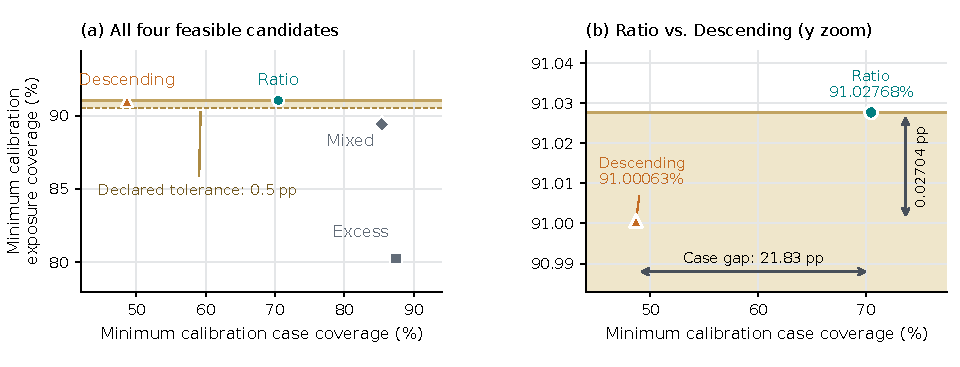
\includegraphics[width=\linewidth]{revision_v8_neartie.pdf}
\caption{Complete-sales 220/220 calibration candidates; Error is infeasible. Minimum case and exposure coverage are taken separately over A/B. The right panel magnifies the exposure axis. Shading marks the illustrative .5-point utility allowance, clipped by the zoom; it is not a confidence interval. Ratio and Descending are close in exposure but far apart in cases.}\label{fig:near-tie}
\end{figure}
\begin{table}[t]\centering\scriptsize
\caption{Complete tolerance grid: exposure-rule choices with original thresholds held fixed. Column values are exposure-coverage allowances in pp. Case choices remain Excess throughout. This is an explicit utility preference, not a confidence region. All candidate metrics and 40 condition outcomes are retained in the accompanying results.}\label{tab:v8-tolerance-grid}
\begin{tabular}{lllllll}\toprule
Arm & Heads & 0 & .1 & .25 & .5 & 1.0\\\midrule
Censored & 220/220 & Descending & Descending & Descending & Descending & Ratio \\
Censored & 660/220 & Descending & Descending & Descending & Descending & Descending \\
Censored & 220/660 & Descending & Descending & Descending & Descending & Ratio \\
Censored & 660/660 & Descending & Descending & Descending & Descending & Descending \\
Complete & 220/220 & Ratio & Ratio & Ratio & Ratio & Ratio \\
Complete & 660/220 & Descending & Descending & Descending & Ratio & Ratio \\
Complete & 220/660 & Descending & Ratio & Ratio & Ratio & Ratio \\
Complete & 660/660 & Descending & Descending & Descending & Ratio & Ratio \\
\bottomrule\end{tabular}\end{table}

\begin{table}[t]\centering\scriptsize
\caption{All eight cells at the declared .5 pp exposure tolerance. Case choice remains Excess. Cal. cost is the minimum-calibration-exposure concession; Later gain/cost compare the tolerance-selected exposure policy with the original exposure choice. Final columns compare the new exposure choice with the unchanged case choice. The .621 pp Later cost in complete 660/220 exceeds the calibration allowance.}\label{tab:v8-tolerance}
\begin{tabular}{llllrrrr}\toprule
Arm & Heads & Original/new & Cal. cost & Later $c$ gain & Later $d$ cost & $\Delta c$ & $\Delta d$\\\midrule
Censored & 220/220 & Descending/Descending & 0.000 & 0.00 & -0.000 & -39.95 & 7.05 \\
Censored & 660/220 & Descending/Descending & 0.000 & 0.00 & -0.000 & -40.66 & 8.29 \\
Censored & 220/660 & Descending/Descending & 0.000 & 0.00 & -0.000 & -37.94 & 8.08 \\
Censored & 660/660 & Descending/Descending & 0.000 & 0.00 & -0.000 & -40.04 & 8.14 \\
Complete & 220/220 & Ratio/Ratio & 0.000 & 0.00 & -0.000 & -15.81 & 9.72 \\
Complete & 660/220 & Descending/Ratio & 0.388 & 24.11 & 0.621 & -10.41 & 10.83 \\
Complete & 220/660 & Descending/Ratio & 0.094 & 13.62 & 0.251 & -21.23 & 9.63 \\
Complete & 660/660 & Descending/Ratio & 0.360 & 19.00 & 0.476 & -15.98 & 10.23 \\
\bottomrule\end{tabular}\end{table}


Table~\ref{tab:v8-tolerance} compares the alternative with both the unchanged case choice and the original exposure choice. One evaluation exposure cost is .6208 pp, exceeding .5; the allowance only bounds the calibration concession.

\paragraph{Analytic intervals.}
For an eligible Ratio candidate $R$, let $D=\max_j\bar d_j$ and $P_j=(\bar c_j,\bar d_j,-j)$, where $j$ is the fixed tie order. Its exact selection interval is
\[
 [L_R,U_R)=\left[D-\bar d_R,\;\min_{j:P_j>_{\rm lex}P_R}(D-\bar d_j)\right).
\]
The upper bound is infinite if there is no higher-priority candidate; the interval is empty if $U_R\leq L_R$ or Ratio is ineligible. The lower bound admits Ratio; the upper bound admits a candidate that defeats it. We check \emph{all} eligible competitors, not just Descending.

For complete-sales 220/220, 660/220, 220/660 and 660/660, the intervals are approximately [0,1.634053), [.388433,2.508229), [.093843,1.646188) and [.360002,2.252009) pp. Mixed supplies every upper endpoint. Their intersection is approximately [.388433,1.634053), containing the conservatively rounded [.39,1.63] pp interval. Thus .5 is not an isolated grid value, but this descriptive interval does not justify selecting a utility from the desired family.

The same 200 complete-reference redesign draws all have nonempty Ratio intervals. Lower-endpoint empirical 2.5/50/97.5 percentiles are 0/0/.479234 pp; upper-endpoint percentiles are .596676/1.643270/3.088298 pp. Exactly 194 contain .5. Bike has 192 nonempty intervals and eight empty ones because Mixed already dominates when Ratio becomes eligible. Nonempty lower endpoints are zero, and upper percentiles are .188918/1.436880/3.550370 pp; .5 belongs to 172 of \emph{all} 200 intervals. These are conditional descriptive endpoint distributions, not confidence bounds. No four-head joint redesign distribution exists in the archive.
\begin{table}[t]\centering\scriptsize
\caption{Exposure-rule frequency (\%) after applying each tolerance to the same 200 threshold-redesign draws from the earlier audit. Fitted scores, cap, $T$, and draw identities are unchanged. The .5 pp rule makes Ratio more frequent in the complete-sales reference and less frequent in Bike; a wider band need not monotonically favor Ratio.}\label{tab:v8-tolerance-frequency}
\begin{tabular}{llrrrrrr}\toprule
Setting & Tolerance pp & Error & Excess & Mixed & Ratio & Desc. & None\\\midrule
Complete 220/220 & 0.00 & 0.0 & 0.0 & 0.0 & 51.5 & 48.5 & 0.0 \\
Complete 220/220 & 0.10 & 0.0 & 0.0 & 0.0 & 69.0 & 31.0 & 0.0 \\
Complete 220/220 & 0.25 & 0.0 & 0.0 & 0.5 & 83.5 & 16.0 & 0.0 \\
Complete 220/220 & 0.50 & 0.0 & 0.0 & 1.5 & 97.0 & 1.5 & 0.0 \\
Complete 220/220 & 1.00 & 0.0 & 0.0 & 16.0 & 83.5 & 0.5 & 0.0 \\
Bike & 0.00 & 0.0 & 0.0 & 4.0 & 96.0 & 0.0 & 0.0 \\
Bike & 0.10 & 0.0 & 0.0 & 4.5 & 95.5 & 0.0 & 0.0 \\
Bike & 0.25 & 0.0 & 0.0 & 8.0 & 92.0 & 0.0 & 0.0 \\
Bike & 0.50 & 0.0 & 0.0 & 14.0 & 86.0 & 0.0 & 0.0 \\
Bike & 1.00 & 0.0 & 0.0 & 34.5 & 65.5 & 0.0 & 0.0 \\
\bottomrule\end{tabular}\end{table}

The source retains all draw intervals and candidate records under \texttt{evidence/revision\_v9\_epsilon/}. Exact-rational breakpoint checks and independent floating-point replay validate the intervals. The implementation's $10^{-12}$ coverage-fraction comparison tolerance moves positive boundaries by only $10^{-10}$ pp. No new fits, threshold searches, resampling draws or evaluation outcomes enter this interval analysis.

\FloatBarrier
\subsection{A-design screening, floors, and exposure allowances}
\label{app:v8-floor}
The floor audit uses .35/.40/.45, four head pairs and five rankings (60 conditions), with reporting/design caps .6326834234/.6010492522 and fitted arrays fixed. Largest feasible whole-tie A thresholds are screened on B using 4,000 item resamples (seed 20260912), at tails .05/60 and .05/20. All 40 nonempty conditions pass (16/12/12 by floor). Exact A utility determines choices before rereading Later data.

Raising the floor either retains the largest risk-feasible threshold or makes its family infeasible; a smaller threshold cannot restore lost case coverage. Descending accepts 35.0483/35.0938\% on A, so even .36 excludes it. Floors .40/.45 select Excess/Ratio throughout, with Later contrasts -26.78 to -16.81 case/+11.59--12.72 exposure points (Table~\ref{tab:v8-floor-main}). Ratio at 220/660 accepts only 45.0574\% on A, limiting extrapolation. The source retains the full 60-condition screen and 24 selected records (48 with both adjustments), including duplicated policies, in \texttt{evidence/revision\_v8\_floor/}; the detailed v8 table files are also retained.

\begin{table}[t]\centering\small
\caption{Complete-sales A-design/B-screen floor sensitivity, all four head pairs per row. Ranges show Later exposure-choice minus case-choice coverage (pp), not confidence intervals. $U_{60}$ is the largest approximate upper risk summary among selected conditions, adjusted over all 60 candidate conditions. Fixed reporting cap is .632683; the same selection occurs under the inherited 20-candidate adjustment.}\label{tab:v8-floor-main}
\begin{tabular}{llllr}\toprule
Floor & Case/exposure rules & $\Delta c$ range & $\Delta d$ range & Max. $U_{60}$\\\midrule
0.35 & Excess/Descending & [-36.39, -35.83] & [12.77, 14.29] & 0.62802 \\
0.40 & Excess/Ratio & [-26.78, -16.81] & [11.59, 12.72] & 0.62756 \\
0.45 & Excess/Ratio & [-26.78, -16.81] & [11.59, 12.72] & 0.62756 \\
\bottomrule\end{tabular}\end{table}


\paragraph{Composing the tolerance rule with screening.}
We now apply the same interval formula to the existing B-passing candidates, using A utility. At floor .35, Descending exceeds Ratio in exposure by 1.083012/1.846934/1.247238/1.597532 pp in the four head settings above. Mixed supplies all upper bounds. The common interval is approximately [1.846934,3.741367) pp: allowances 0/.5/1 retain Descending throughout, whereas 2 selects Ratio throughout. At floors .40/.45, the common Ratio interval is [0,2.494129) pp, so all four tested allowances select Ratio. Both screen-family adjustments agree. All conditions and breakpoint checks are retained in \texttt{evidence/revision\_v9\_screen\_tolerance/}.

The near-tie result for the original joint-A/B design does not extend to this stricter A-only design. Under the illustrative .5 pp allowance, its family switch is caused by the floor restriction; a larger declared concession supplies a different route. This establishes neither a universal allowance nor the causal effect of changing the design cap alone. Selected Later upper summaries remain approximate and fit-conditional: the largest $U_{60}=.62802431<r$, but .05/60 in 4,000 draws leaves only about 3.3 draws in the tail. Union risk and prospective generalization are not evaluated.

\section{Additional seeds and an external analysis frozen before data opening}
\label{app:additional-v12}
\subsection{Additional paired seeds}\label{app:seeds-v12}
Two seeds (20260913 and 20260914) were fixed after inspecting the original 20260910 results. Each repeats ten fits: two 300-tree median predictors and eight 220/660-tree squared-loss heads. Original periods, 600,000-row sampling, features, and parameters are retained. The seed changes row sampling and bin construction; both arms share the sampled rows within a seed. The item-bootstrap seed is held at 20260910 (2,000 draws) to separate its Monte Carlo variation from refitting. The cap formula remains .95 times maximum full A/B calibration risk per arm. These repetitions use the same previously evaluated M5 data; they are not three new external confirmation trials.

Table~\ref{tab:seed-v12-all} reports all 24 seed/cells. Original calibration stability, tolerance, floor, exchange-interval and budget audits retain seed 20260910; they are not rerun or averaged across the additional seeds. Original per-cell point values also remain in Table~\ref{tab:matched-heads}. One saved calibration NPZ in seed 20260914 was incomplete despite matching its original completion hash. Its seven arrays were replayed from the frozen models without fitting; all four surviving arrays matched exactly and original threshold/results records were retained. The original archive and recovery protocol are supplied in the source. New evidence and independent checks are in \texttt{evidence/revision\_v12\_seeds/} and \texttt{docs/revision\_v12/}.

\begin{table}[H]\centering\small
\caption{Every paired seed/cell. Seed suffixes 10, 13, 14 mean 20260910, 20260913, 20260914. Censored and complete are abbreviated C and F. Case choice is Excess throughout. These are point effects in percentage points, not independent dataset replications.}\label{tab:seed-v12-all}
\begin{tabular}{cllcrrr}\toprule
Seed & Arm & Heads & Exposure & Cap & $\Delta c$ & $\Delta d$\\\midrule
10 & C & 220/220 & Descending & 0.66471 & -39.95 & +7.05 \\
10 & C & 660/220 & Descending & 0.66471 & -40.66 & +8.29 \\
10 & C & 220/660 & Descending & 0.66471 & -37.94 & +8.08 \\
10 & C & 660/660 & Descending & 0.66471 & -40.04 & +8.14 \\
10 & F & 220/220 & Ratio & 0.63268 & -15.81 & +9.72 \\
10 & F & 660/220 & Descending & 0.63268 & -34.52 & +11.45 \\
10 & F & 220/660 & Descending & 0.63268 & -34.85 & +9.88 \\
10 & F & 660/660 & Descending & 0.63268 & -34.98 & +10.71 \\
13 & C & 220/220 & Descending & 0.66469 & -38.71 & +8.31 \\
13 & C & 660/220 & Descending & 0.66469 & -40.47 & +8.26 \\
13 & C & 220/660 & Descending & 0.66469 & -35.97 & +9.80 \\
13 & C & 660/660 & Descending & 0.66469 & -39.14 & +8.49 \\
13 & F & 220/220 & Ratio & 0.63357 & -18.28 & +8.42 \\
13 & F & 660/220 & Descending & 0.63357 & -35.86 & +9.74 \\
13 & F & 220/660 & Ratio & 0.63357 & -23.03 & +7.78 \\
13 & F & 660/660 & Descending & 0.63357 & -36.54 & +8.14 \\
14 & C & 220/220 & Descending & 0.66517 & -37.62 & +9.84 \\
14 & C & 660/220 & Descending & 0.66517 & -38.25 & +11.19 \\
14 & C & 220/660 & Descending & 0.66517 & -35.71 & +10.21 \\
14 & C & 660/660 & Descending & 0.66517 & -37.75 & +10.38 \\
14 & F & 220/220 & Descending & 0.63328 & -34.74 & +10.88 \\
14 & F & 660/220 & Descending & 0.63328 & -34.01 & +12.05 \\
14 & F & 220/660 & Descending & 0.63328 & -34.71 & +10.18 \\
14 & F & 660/660 & Descending & 0.63328 & -34.56 & +10.78 \\
\bottomrule\end{tabular}\end{table}

\subsection{External protocol and complete candidate report}\label{app:external-v12}
We thank the James M. Kilts Center for Marketing at the University of Chicago Booth School of Business for the Dominick's data. This academic analysis uses the Oatmeal movement CSV, selected for public access and bounded scope before raw outcomes were opened. Favorita was considered but not downloaded because authentication was unavailable. No outcome-based choice between datasets or categories was made. No earlier use of Dominick's was found in the study records. The protocol is a local, time-stamped pre-opening record, not a public-registry preregistration.

Weeks 53--208 fit the point predictor; 209--260 fit heads; 261--312 are A; 313--364 are B; 365--400 are final evaluation. Valid records have the provider's OK flag equal to one and finite nonnegative MOVE. Missing records are not imputed as sales. The cohort requires at least 52 valid point-training records and positive point-training sales, with no future-window selection. It contains 4,839 store--UPC series, 66 products and 86 stores. Point/head/A/B/evaluation record counts are 511,980/186,347/153,255/139,881/85,039.

Forecasts are rolling one week ahead. Features are store/UPC identifiers, time, seasonal sine/cosine, sales lags 1/2/4/13/26/52, and past-only rolling means, standard deviations, maxima and missing fractions over 4/13/26 weeks. The 300-tree median predictor and two 220-tree squared-loss heads use seed 20260912 and the paired study's learning rate, leaf count and minimum leaf size. No tuning or early stopping is performed. A determines $r=.95R_{\rm all,A}=.91739424$ and thresholds at $.95r=.87152453$, floor .40. Each utility selects on A; B only screens the fixed choices, without fallback or reselection.

Circular moving blocks of four calendar weeks retain all UPC/store records in each week; B and evaluation use 20,000 draws each, with separate fixed seeds. Five-candidate upper risk summaries use tail .05/5. The declared joint success criterion requires both A-selected policies to pass B and the final 95\% paired intervals to have upper $\Delta c<0$ and lower $\Delta d>0$. It is not met: $\Delta c=-4.6343$ ($[-6.1496,-3.4492]$) and $\Delta d=2.5299$ ($[-.6887,5.8453]$). Positive point direction and B passage provide partial evidence, but not the declared interval confirmation. No retuning followed.

An overstrict implementation assertion initially stopped evaluation because weeks 370, 371 and 400 had no records. The completion retains all 36 calendar weeks with zero contribution in empty weeks, using the same frozen policies, models, arrays, bootstrap settings and success criterion. It performs no new fits or selection and reproduces the existing B results exactly. Original failure and amendment records are preserved. This does not change the observational meaning of missing weeks or give a population guarantee.

\begin{table}[H]\centering\small
\caption{All five external candidates. Coverages are percentages. A risk design uses .871525; B compares its adjusted upper risk summary with .917394. Descending is infeasible on A; Error is feasible on A but fails B. Selected Excess and Ratio both pass B.}\label{tab:external-v12-all}
\begin{tabular}{lrrcrrr}\toprule
Rule & A $c$ & A $d$ & B risk upper & E $c$ & E $d$ & E risk\\\midrule
Excess & 94.57 & 77.95 & 0.90950 & 96.29 & 89.68 & 0.82991 \\
Ratio & 85.27 & 86.15 & 0.87573 & 91.65 & 92.21 & 0.82070 \\
Descending & 0.00 & 0.00 & -- & 0.00 & 0.00 & -- \\
Mixed & 93.29 & 85.06 & 0.87381 & 94.52 & 91.81 & 0.81972 \\
Error & 93.66 & 71.53 & 0.94596 & 95.08 & 82.08 & 0.83644 \\
\bottomrule\end{tabular}\end{table}

\section{Decision-level sensitivity of estimated constraints}
\label{app:plugin-v12}
Appendix~\ref{app:proofs} bounds score perturbations. Moving from scores to
decisions additionally requires stability of the feasible set. Constraint
tightening under strict feasibility is established in constrained learning
\citep[Proposition 4.1]{rigollet2011strict}; consistent plug-in methods also
exist for general confusion-matrix objectives and constraints
\citep{tavker2020plugin}. The result below specializes this sensitivity
argument to accepted exposure and ratio risk. We do not claim a new general
plug-in framework or use the result to certify our empirical policies.

Fix a distribution and nonnegative integrable conditional moments $\ell,w$
with $T=\E w>0$. For a gate $a$, write
$M(a)=\E[aw]$ and $G(a)=\E[a(\ell-rw)]$, where $r\geq0$.
Use hats for the same expectations with estimated moments. A common convex
class $\mathcal A\subseteq\{a:0\leq a\leq1\}$ may include the true case floor.
Suppose
\[
 \sup_{a\in\mathcal A}|\widehat M(a)-M(a)|\leq\epsilon_M,
 \qquad
 \sup_{a\in\mathcal A}|\widehat G(a)-G(a)|\leq\epsilon_G.
\]
Sufficient choices are $\epsilon_M=\E|\widehat w-w|$ and
$\epsilon_G=\E|\widehat\ell-\ell|+r\E|\widehat w-w|$.

\begin{proposition}[Buffered plug-in sensitivity]
\label{prop:plugin-v12}
Assume a maximizer $a^*$ of $M(a)$ subject to $a\in\mathcal A$, $G(a)\leq0$
exists, and some $a_0\in\mathcal A$ satisfies $G(a_0)\leq-s<0$.
Let $\widehat a$ be an $\eta$-optimal solution maximizing $\widehat M$
subject to $\widehat G\leq-\tau$, where $\eta,\tau\geq0$ and
$\epsilon_G+\tau\leq s$. Then
\begin{align}
 d_W(a^*)-d_W(\widehat a)
 &\leq\frac{\epsilon_G+\tau}{s}
       +\frac{2\epsilon_M+\eta}{T},\label{eq:plugin-cover-v12}\\
 G(\widehat a)&\leq\epsilon_G-\tau.\label{eq:plugin-excess-v12}
\end{align}
If $M(\widehat a)\geq m_0>0$, then
$[R(\widehat a)-r]_+\leq(\epsilon_G-\tau)_+/m_0$.
In particular, $\tau=\epsilon_G$ ensures true feasibility when
$2\epsilon_G\leq s$ and accepted exposure is positive.
\end{proposition}

\begin{proof}
Set $t=(\epsilon_G+\tau)/s\in[0,1]$ and
$a_t=(1-t)a^*+ta_0\in\mathcal A$. Linearity gives
$G(a_t)\leq-ts$, hence $\widehat G(a_t)\leq-\tau$.
Optimality up to $\eta$ and the objective error bound give
\[
 M(\widehat a)\geq\widehat M(\widehat a)-\epsilon_M
 \geq\widehat M(a_t)-\eta-\epsilon_M
 \geq M(a_t)-2\epsilon_M-\eta.
\]
Thus $M(a^*)-M(\widehat a)\leq
t\{M(a^*)-M(a_0)\}+2\epsilon_M+\eta$.
Since $a_0$ is feasible, $0\leq M(a^*)-M(a_0)\leq T$.
Equation~\eqref{eq:plugin-excess-v12} follows from feasibility of
$\widehat a$ for the estimated problem and the constraint error bound.
Dividing by positive $M(\widehat a)$ proves the risk statement.
\end{proof}

The unbuffered output can be truly infeasible, so the coverage shortfall in
Equation~\eqref{eq:plugin-cover-v12} need not be nonnegative. A case floor
alone does not give $m_0$ if $w$ approaches zero. The stronger condition
$w\geq u>0$, $c(a)\geq c_0>0$ gives $m_0=uc_0$.

\paragraph{A finite-menu corollary and its scope.}
For a common finite class, convexity is unnecessary if a true comparator
$a^*$ satisfies $G(a^*)\leq-(\epsilon_G+\tau)$: it remains feasible for
the estimated problem, and the same comparison yields
$M(a^*)-M(\widehat a)\leq2\epsilon_M+\eta$.
The empirical procedure uses fitted heads to propose rankings, but observed
calibration losses to set thresholds. Its five candidates are not closed
under mixtures. Applying either result to that procedure would require
uniform errors for the relevant data-dependent criteria, robustness of
candidate eligibility, and (for oracle comparison) class approximation
control. These assumptions are not supplied by the reported bootstrap
intervals. Changing fitted heads also changes the candidate class.

\paragraph{Why head accuracy alone is insufficient.}
Let two contexts have equal probability, $w=1$ and $\ell=r>0$ in both.
Accept-all is truly feasible. Set $\widehat w=1$ and
$\widehat\ell=(r+\varepsilon,r-\varepsilon^2)$ with
$0<\varepsilon<\min(1,\sqrt r)$. The plug-in optimum accepts the second
context and an $\varepsilon$ fraction of the first, since its constraint
is $\varepsilon a_1\leq\varepsilon^2a_2$.
Its coverage is $(1+\varepsilon)/2$, so its shortfall tends to $1/2$
despite vanishing uniform head error and accepted exposure at least $1/2$.
It meets a .35 case floor and has true risk exactly $r$. No gate has strict
true slack. Hence head error and a positive denominator alone cannot imply
vanishing coverage regret.

For a separate denominator example, let two equally likely contexts have
$w=(2\varepsilon,2(1-\varepsilon))$ and
$\ell=(2(r+1)\varepsilon,2(r+2)(1-\varepsilon))$.
Estimate only the first loss as $2r\varepsilon$. The plug-in optimum
accepts only that context. The loss-head $L^1$ error is $\varepsilon$,
total exposure is one, and case coverage is $1/2$, yet accepted exposure
is $\varepsilon$ and true risk is $r+1$. This example concerns risk
certification; it does not posit a true positive-exposure feasible gate.

Neither example establishes why Descending beats Ratio in M5. Moment errors
can cancel in the ratio, and empirical eligibility and time shift introduce
additional effects. The new result identifies sufficient conditions and
limits of a plug-in guarantee; the empirical estimation mechanism remains
unidentified.

\FloatBarrier
% Integrated Appendix N. Tables are derived from retained v13 JSON records.
% All v13 labels are namespaced. Requires the main paper's amsmath/booktabs/float packages.
\section{Frozen non-WAPE tests and learned gates}
\label{app:v13-nonwape}

\subsection{Scope, prediction sets, and the frozen design}
\label{sec:v13-design}
These two external tests examine fixed multi-label prediction with whole-example abstention. They were specified after the M5 and Dominick's results were known; they neither replace the Dominick's trial nor turn the earlier analyses into prospective evidence. Bibtex and Mediamill were both selected before raw acquisition, with no result-based replacement. A local timestamped protocol and five implementation files were frozen before either raw archive was downloaded. Public benchmark metadata, including label cardinalities, had been seen. This is a before-download code/protocol freeze, not public-registry preregistration or a claim that all public information was unseen.

We use the official Mulan train/test archives, retaining their partitions. Within official training rows, a label-independent SHA256 ordering assigns the first $\lfloor .7n\rfloor$ rows to predictor training T and the remainder to head/gate training H. Within official test rows, the first and second $\lfloor n/3\rfloor$ rows are A and B; the remainder form final evaluation E (Later). Table~\ref{tab:v13-roles} gives every role size. Hash inputs consist of a frozen study identifier, dataset, original partition, and source row index. These are hash splits, not chronological windows. Raw parsing materializes labels; the separation is in their use for fitting, design, screening, and evaluation. A policy records precede B calculations, which precede E calculations.

\begin{table}[H]\centering\small
\caption{Non-WAPE data and role sizes. $p$ is the feature count and $K$ the label count. Official train/test totals are 4,880/2,515 for Bibtex and 30,993/12,914 for Mediamill.}
\label{tab:v13-roles}
\begin{tabular}{lrrrrrrr}\toprule
Dataset & $p$ & $K$ & T & H & A & B & E\\\midrule
Bibtex & 1836 & 159 & 3,416 & 1,464 & 838 & 838 & 839 \\
Mediamill & 120 & 101 & 21,695 & 9,298 & 4,304 & 4,304 & 4,306 \\
\bottomrule\end{tabular}
\end{table}

For each label, an L2 logistic classifier uses $C=1$, the liblinear solver, tolerance $10^{-4}$, at most 1,000 iterations, and no class weights. Feature scaling is fitted on T only, without centering. A label constant on T receives probability $(n_{+,T}+1)/(n_T+2)$. We retain labels with predicted probability at least $.5$. If this set is empty, the maximum-probability label is retained, with source label order resolving exact ties. This forced top-one convention was frozen in advance; it differs from the earlier Yeast convention that freely accepts zero-loss, zero-exposure examples. It ensures a nonempty set and hence a defined positive exposure for every row, but also changes the base prediction task. It is therefore part of the result's scope, not innocuous numerical preprocessing.

For a fixed predicted-label set, $w$ is its size and $\ell$ is the number of false positives. Whole-example acceptance keeps or rejects the complete set. The ratio $\sum_i a_i\ell_i/\sum_i a_iw_i$ is one minus micro-precision. Exposure coverage measures retained predicted positives, not recall or coverage of true labels. Unlike retail demand, $w\geq1$ is exactly known when deciding whether to accept; no exposure head is fitted. The error head is an ExtraTrees regressor fitted on H with 220 trees, at most 31 leaves per tree, minimum leaf size 10, all features available, no bootstrap, and predictions clipped to $[0,w]$. Every selector uses the same T-scaled features augmented with $\log(1+w)$. Dataset seeds are 20260913 and 20260914, respectively. There is one classifier seed per dataset and no validation tuning or early stopping; no classifier convergence warning was recorded.

The five ascending scores are Error $\hat e$, Excess $\hat e-rw$, Ratio $\hat e/w$, Descending $-w$, and
\begin{equation}
 s_{\lambda}(x)=\frac{\hat e(x)-rw(x)}{\lambda+(1-\lambda)w(x)/\bar w_H},
 \qquad \lambda=.5,\qquad \bar w_H=|H|^{-1}\sum_{i\in H}w_i.
 \label{eq:v13-mixed}
\end{equation}
The case coefficient $\lambda=.5$ was frozen for these two tests. The earlier retail menu, including Dominick's, uses $\lambda=.25$ in Eq.~\ref{eq:mixed}; that value is examined separately in Section~\ref{sec:v13-lambda}. No denominator floor or tolerance-band alternative enters the frozen tests.

A alone sets $r=.95R_{\mathrm{all},A}$: $.44285714$ for Bibtex and $.22880705$ for Mediamill. Each score retains its largest A-feasible prefix at design risk $.95r$ and case coverage at least $.40$. The design caps are $.42071429$ and $.21736670$. A common outcome-independent hash orders score ties; the stored boundary is a score/hash pair. Utility selects among eligible menu members by A case or exposure coverage, with exact utility ties resolved in the declared order Error, Excess, Mixed, Ratio, Descending. The two custom learned gates use the same A feasibility rule. These cap, tightening, and floor conventions agree with Dominick's; they differ from the primary M5 cap based on both A and B and its $.35$ floor. Shared cap conventions do not make the tasks, tie handling, sampling units, or uncertainty families identical. We preserve each frozen design rather than retuning it for agreement across datasets.

\subsection{Learned-gate comparator}
\label{sec:v13-gate-design}
The comparator is a custom primal-dual multilayer perceptron with 32 and 16 ReLU hidden units and a sigmoid acceptance output $a_\theta$. GateCase and GateExposure share initialization within each dataset. The predictor remains fixed. Training uses H rows, with the A-derived cap entering only as a scalar. For $u_i=1$ or $w_i/\bar w_H$, the objective is
\begin{equation}
 -\overline{a_\theta u}_{H}
 +\alpha\,\frac{\overline{a_\theta(\ell-rw)}_{H}}{\bar w_H}
 +\gamma\bigl(.40-\overline{a_\theta}_{H}\bigr),
 \qquad \alpha,\gamma\geq0.
 \label{eq:v13-gate-objective}
\end{equation}
The 40-epoch, float64 training uses minibatch Adam with batch size 2,048, learning rate $.003$, weight decay $.0001$, gradient norm clipping at 5, and feature clipping to $[-10,10]$. Once per epoch, full-H dual ascent has step $.2$ and duals clipped to $[0,100]$, starting at $\alpha=\min(1/r,100)$ and $\gamma=0$. Negative gate logits define ascending scores for the same A threshold search. Training traces and all fitted weights are retained. This is a fixed-predictor learned-selector comparison, not a SelectiveNet reproduction, joint predictor training, or evidence that the soft optimization converged to a constrained optimum. One untuned architecture cannot establish the relative merits of learned selectors in general.

\subsection{Screening, contrasts, and all candidate outcomes}
\label{sec:v13-inference}
B screens the already fixed policies without fallback or reselection. Its statistic is the mean signed excess
\begin{equation}
 \widehat G_B(a)=\frac{1}{n_B}\sum_{i\in B}a_i(\ell_i-rw_i).
 \label{eq:v13-signed-screen}
\end{equation}
The paired row multinomial bootstrap uses 20,000 draws and the linear-interpolated upper quantile $1-.05/14=.9964285714$, retaining the declared family of seven candidates on each of two datasets even when a candidate is A-ineligible. A pass requires A eligibility, positive accepted exposure in every resample, and upper $\widehat G_B<0$. Table~\ref{tab:v13-candidates} reports B point risk alongside this upper bound. The bound is in false-positive-count units per row, not risk units; it is compared with zero, not with $r$.

E uses 20,000 paired row resamples, independently seeded from B. Exposure coverage is recomputed as the ratio of resampled sums. The four primary contrasts (two utilities, two datasets) use marginal 98.75\% intervals, with quantiles $.00625$ and $.99375$. The eight declared gate-minus-menu slots use marginal 99.375\% intervals, with quantiles $.003125$ and $.996875$; two slots remain unavailable because Mediamill GateCase is A-ineligible. Each of these two contrast families and the B screen is adjusted separately. They do not combine into one simultaneous 95\% claim, nor do these bootstrap summaries establish population risk control. Bootstrap seeds are the dataset seed times 100 plus 1 for B and plus 2 for E.

The declared dataset-level joint criterion requires both A-selected menu policies to pass B and the primary E intervals to satisfy upper $\Delta c<0$ and lower $\Delta d>0$. Cross-dataset success requires both datasets to satisfy it. Bibtex passes both selected-policy screens but its exposure-gain interval includes zero. Mediamill has both directional intervals excluding zero, but both selected policies fail B. Thus neither dataset, nor their conjunction, meets the declared criterion. Results after failed screens remain reported; they are not promoted to screen-approved policies.

\begin{table}[H]\centering\small
\setlength{\tabcolsep}{4pt}
\caption{All seven declared candidates per dataset, with frozen $\lambda=.5$. Coverages on E are percentages; risk is FP divided by predicted-positive mass. An A-ineligible candidate has no selected threshold and is shown as unavailable, not as an evaluated reject-all policy. Selected menu pairs are Excess/Ratio (Bibtex) and Excess/Mixed (Mediamill).}
\label{tab:v13-candidates}
\begin{tabular}{lrrcrrr}\toprule
Policy & B risk & B upper $G$ & B status & E $c$ & E $d$ & E risk\\\midrule
\multicolumn{7}{l}{\textit{Bibtex}}\\
Error & 0.40258 & +0.00794 & Fail & 72.47 & 57.87 & 0.36259 \\
Excess & 0.38342 & -0.01385 & Pass & 80.21 & 78.10 & 0.40405 \\
Mixed & 0.37410 & -0.02598 & Pass & 77.83 & 79.35 & 0.41028 \\
Ratio & 0.37551 & -0.02334 & Pass & 75.80 & 80.10 & 0.41060 \\
Descending & -- & -- & A-ineligible & -- & -- & -- \\
GateCase & 0.40247 & +0.00424 & Fail & 86.77 & 85.10 & 0.39922 \\
GateExposure & 0.40116 & +0.00634 & Fail & 83.08 & 84.68 & 0.39528 \\
\midrule
\multicolumn{7}{l}{\textit{Mediamill}}\\
Error & 0.22627 & +0.02335 & Fail & 87.02 & 78.40 & 0.21451 \\
Excess & 0.22397 & +0.01908 & Fail & 89.36 & 85.45 & 0.21507 \\
Mixed & 0.22769 & +0.02756 & Fail & 86.23 & 87.86 & 0.21603 \\
Ratio & 0.22450 & +0.02064 & Fail & 82.72 & 87.74 & 0.21621 \\
Descending & -- & -- & A-ineligible & -- & -- & -- \\
GateCase & -- & -- & A-ineligible & -- & -- & -- \\
GateExposure & 0.22988 & +0.03337 & Fail & 84.42 & 89.00 & 0.22423 \\
\bottomrule\end{tabular}
\end{table}

\begin{table}[H]\centering\small
\setlength{\tabcolsep}{3pt}
\caption{Frozen paired E contrasts in percentage points. Primary menu rows are exposure-choice minus case-choice, with 98.75\% marginal intervals. Gate rows are gate minus the menu choice for the same utility, with 99.375\% marginal intervals. B status refers to the two policies in that row. These are two separately adjusted contrast families; neither dataset meets the joint primary criterion.}
\label{tab:v13-contrasts}
\begin{tabular}{lccc}\toprule
Contrast & $\Delta c$ [interval] & $\Delta d$ [interval] & B passes\\\midrule
Bibtex menu & $-4.41\ [-7.39,-1.55]$ & $+2.00\ [-1.84,+6.08]$ & Both \\
Mediamill menu & $-3.14\ [-4.27,-2.02]$ & $+2.40\ [+1.31,+3.57]$ & Neither \\
\midrule
Bibtex gate (case) & $+6.56\ [+1.91,+11.44]$ & $+6.99\ [+0.76,+13.07]$ & Menu only \\
Bibtex gate (exposure) & $+7.27\ [+2.56,+12.16]$ & $+4.58\ [-0.77,+9.89]$ & Menu only \\
Mediamill gate (case) & -- & -- & A-ineligible \\
Mediamill gate (exposure) & $-1.81\ [-3.48,-0.12]$ & $+1.15\ [-0.81,+3.09]$ & Neither \\
\bottomrule\end{tabular}
\end{table}

Bibtex GateCase has higher E case and exposure coverage than Excess by 6.56 and 6.99 points, and lower point risk ($.39922$ versus $.40405$). Both coverage intervals in its secondary family exclude zero. Its B risk, however, is higher ($.40247$ versus $.38342$), and its signed-excess upper bound is $+.00424$ rather than Excess's $-.01385$. The corresponding B mean excesses are $-.05065$ and $-.06845$. The later advantage is visible, but this gate does not meet the declared screen. The observed policies accept different sets, so these summaries alone establish neither a gate-specific causal defect nor an explanation solely in terms of low screening power. Mediamill GateExposure also fails B; its exposure contrast with Mixed includes zero. No screened learned-gate superiority is established, and no general menu superiority follows.

\subsection{Realized split risks and Descending feasibility}
\label{sec:v13-split-diagnostics}
The following diagnostics were computed after the frozen outcomes were known. Table~\ref{tab:v13-split-risk} places full-coverage risk across A/B/E next to each fixed cap. Bibtex B is easier than A by 3.78 risk percentage points, whereas Mediamill B is harder by .73 points. The latter is consistent with a less favorable screening split, but the label-independent hash partitions are not temporal windows: these differences do not establish distributional drift or identify the cause of screen failure. In Mediamill, all four eligible menu candidates have B point risks below $r$, yet all their upper signed-excess bounds cross zero. Failed confirmation is therefore distinct from an established violation of the cap.

\begin{table}[H]\centering\small
\setlength{\tabcolsep}{4pt}
\caption{Post hoc context for B screening. Full risks use all rows in each split. The final column is the minimum A risk among \emph{every} Descending prefix satisfying the $.40$ case floor; it exceeds $r$ in both datasets, even before the additional $.95r$ design tightening.}
\label{tab:v13-split-risk}
\begin{tabular}{lrrrrrr}\toprule
Dataset & Full A & Full B & Full E & B/A & $r$ & Min. Desc. A\\\midrule
Bibtex & 0.46617 & 0.42833 & 0.43464 & 0.9188 & 0.44286 & 0.45733 \\
Mediamill & 0.24085 & 0.24819 & 0.23939 & 1.0305 & 0.22881 & 0.23120 \\
\bottomrule\end{tabular}
\end{table}

Descending is consequently A-ineligible, unlike the common exposure choice in the M5 audit. The exact prefix minima are $418/914=.4573304$ for Bibtex and $2416/10450=.2311962$ for Mediamill. This establishes a feasibility fact for these fitted classifiers and fixed rankings. It does not identify why false positives occur at particular predicted-positive counts. The available frozen protocol, code, and archived design memo contain no documented prospective power calculation or power-based sample-size choice for these two tests. Interval width depends on the paired policy differences and sampling assumptions as well as $n$; the sample size alone does not establish that a two-point gain was impossible to detect. These diagnostics do not change either joint-success decision.

\subsection{The Mixed convention: frozen result and post hoc sensitivity}
\label{sec:v13-lambda}
Equation~\ref{eq:v13-mixed} defines $\lambda$ as the case-utility coefficient. Thus the historical $\lambda=.25$ convention has denominator $.25+.75w/\bar w_H$, while the frozen non-WAPE convention has $.5+.5w/\bar w_H$. We retain the latter as the primary analysis. The sensitivity reuses the fitted classifier, error head, H normalization, cap, floor, and hash order, recalibrates the changed Mixed score on A, and reapplies the declared menu choice. It uses the same B/E resampling seeds. It is post hoc and adds no confirmatory evidence to the original families. Table~\ref{tab:v13-lambda} includes both quarter-weight orientations that were calculated, avoiding selective retention of one convention.

\begin{table}[H]\centering\small
\setlength{\tabcolsep}{3pt}
\caption{Mixed-coefficient sensitivity. $\lambda$ weights case utility; C/D are case/exposure menu choices (Ex=Excess, Mix=Mixed, R=Ratio). The $.5$ rows reproduce frozen primary results; $.25$ and $.75$ are post hoc. Their displayed 98.75\% intervals are descriptive and outside the original confirmatory family. ``Both B'' means satisfying the original numerical screen rule, not a newly approved confirmatory screen. No row satisfies all original joint inequalities.}
\label{tab:v13-lambda}
\begin{tabular}{lccccc}\toprule
Dataset & $\lambda$ & C/D & $\Delta c$ [interval] & $\Delta d$ [interval] & Both B\\\midrule
Bibtex & 0.50 & Ex/R & $-4.41\ [-7.39,-1.55]$ & $+2.00\ [-1.84,+6.08]$ & Yes \\
Bibtex & 0.25 & Ex/Mix & $-1.67\ [-4.05,+0.72]$ & $+2.75\ [-0.41,+6.30]$ & Yes \\
Bibtex & 0.75 & Mix/R & $-5.60\ [-8.34,-2.98]$ & $-0.50\ [-3.81,+3.05]$ & Yes \\
\midrule
Mediamill & 0.50 & Ex/Mix & $-3.14\ [-4.27,-2.02]$ & $+2.40\ [+1.31,+3.57]$ & No \\
Mediamill & 0.25 & Ex/Mix & $-5.53\ [-6.83,-4.23]$ & $+2.39\ [+1.11,+3.73]$ & No \\
Mediamill & 0.75 & Ex/R & $-6.64\ [-8.04,-5.29]$ & $+2.29\ [+0.95,+3.67]$ & No \\
\bottomrule\end{tabular}
\end{table}

At $\lambda=.25$, Bibtex's exposure choice changes from Ratio to Mixed, and even the case-difference interval includes zero. Mediamill retains a directional exchange but still fails B. The conclusion is therefore sensitive to the menu convention in Bibtex; the frozen result is not silently replaced with the historical coefficient. The sensitivity files use an exposure-weight parameter $1-\lambda$, so their key \texttt{0.75} corresponds to the paper's $\lambda=.25$.

\subsection{Forced top-one rows and fixed-policy subgroup accounting}
\label{sec:v13-fallback}
Saved classifier probabilities identify rows whose original $.5$ prediction set was empty. After reconstructing these flags, we hold every fitted object, selected rule, threshold, cap, floor, and acceptance mask fixed and condition evaluation on fallback status. This is a post hoc change in the evaluation population. It does not refit a classifier without fallback, redesign its selectors, provide a causal estimate of the convention's effect, or repeat B screening on the restricted cohort. No subgroup interval or new success claim is attached.

\begin{table}[H]\centering\small
\setlength{\tabcolsep}{4pt}
\caption{Frozen exposure-choice minus case-choice accounting on E. Net cases and net exposure are differences in accepted counts and predicted-positive mass. Percentage-point differences use the indicated cohort's own denominators; they must not be added across cohorts. The raw net counts and masses do add.}
\label{tab:v13-fallback}
\begin{tabular}{llrrrrr}\toprule
Dataset & Cohort & $n$ & Net cases & Net exposure & $\Delta c$ & $\Delta d$\\\midrule
Bibtex & All & 839 & -37 & +24 & -4.41 & +2.00 \\
Bibtex & Forced top-one & 273 & -41 & -41 & -15.02 & -15.02 \\
Bibtex & Nonfallback & 566 & +4 & +65 & +0.71 & +7.00 \\
\midrule
Mediamill & All & 4,306 & -135 & +268 & -3.14 & +2.40 \\
Mediamill & Forced top-one & 137 & -61 & -61 & -44.53 & -44.53 \\
Mediamill & Nonfallback & 4,169 & -74 & +329 & -1.78 & +2.99 \\
\bottomrule\end{tabular}
\end{table}

In Bibtex, the 273 forced rows contribute $-41$ accepted cases, offset by $+4$ among 566 nonfallback rows; the total is $-37$. Their exposure contributions are $-41$ and $+65$, totaling $+24$ out of 1,201 predicted positives. Thus Bibtex's \emph{net case loss is confined to forced single-label rows}. The nonfallback cohort has gains in both coverages ($+.71/ +7.00$ points); the case/exposure exchange does not persist there. Within the fallback cohort $w=1$, Ratio and Excess are $\hat e$ and $\hat e-r$ and share an ordering, including their hash tie order. Different global thresholds create the accepted-count difference. Both coverages fall equally within that cohort; the entire aggregate exchange is not an exchange within forced rows. This limits Bibtex's evidence for the task without the fallback convention.

Mediamill's nonfallback cohort instead retains a point exchange of $-1.78/ +2.99$ points over 4,169 examples. This is evidence that its descriptive exchange is not confined to the 137 forced rows. It neither repairs the failed B screen nor turns this subgroup into a new frozen trial. Of these two new non-WAPE datasets, Mediamill alone retains an opposite-sign point contrast after conditioning away forced predictions.

\subsection{Exposure distribution and inference limits}
\label{sec:v13-exposure}
Table~\ref{tab:v13-exposure} records the already-evaluated E exposure distributions. We do not use them to claim that cross-dataset effect size follows exposure dispersion. Bibtex has the larger coefficient of variation and observed max/min ratio, whereas Mediamill has the larger 95th/5th percentile ratio. Selecting a dispersion summary after seeing the effects could manufacture an apparent ordering. The bounded-exposure theorem is an upper envelope under support assumptions, not a prediction of realized effect size, a lower bound on reversal, or a power calculation. Empirical quantiles are not population support bounds. The earlier proposed monotone dispersion explanation is therefore not retained.

\begin{table}[H]\centering\small
\setlength{\tabcolsep}{4pt}
\caption{Post hoc E exposure summaries. SD uses the population divisor; CV=SD/mean. $w=1$ includes naturally single-label predictions as well as forced rows, and must not be equated with fallback. Both percentages use all E rows.}
\label{tab:v13-exposure}
\begin{tabular}{lrrrrrrr}\toprule
Dataset & Mean & SD & CV & $q_{.05}/q_{.5}/q_{.95}$ & Min--max & $w=1$ (\%) & Forced (\%)\\\midrule
Bibtex & 1.431 & 1.039 & 0.726 & 1/1/3 & 1--19 & 73.54 & 32.54 \\
Mediamill & 2.589 & 1.166 & 0.450 & 1/2/5 & 1--9 & 12.77 & 3.18 \\
\bottomrule\end{tabular}
\end{table}

All uncertainty summaries condition on the fitted models and A design and use a row-exchangeability approximation. Exact feature duplicates are retained under the frozen no-exclusion rule: Bibtex has duplicates within and across roles, including between A/B and B/E; Mediamill has training-role duplicates, and the distributed files do not provide grouping identifiers that would support video/shot cluster inference. Absence of exact duplicates in a role does not establish independence. The bootstrap omits classifier and split variability, and these two tests have one classifier seed each. The M5 three-seed audit does not remove those limitations.

The anonymous supplement retains the frozen protocol, acquisition and source hashes, original A/B/E arrays, fitted objects, full training traces, bootstrap draws, and independent verification code. Post hoc coefficient and subgroup diagnostics are separated from the frozen evidence. Raw Mulan archives are not redistributed; their recorded source locations and hashes support reacquisition. Historical status strings in unchanged freeze or follow-up records describe the state when those records were written; the integrated definitions and conventions above specify the current manuscript. Neither the negative joint outcomes nor the unfavorable learned-gate screening results are omitted.

\end{document}
